\documentclass[11pt, a4paper]{article}

\usepackage[T1]{fontenc}

%\usepackage[utf8]{inputenc}
\usepackage{authblk}
\usepackage{graphicx}
%\usepackage[title]{appendix}
\usepackage{amsmath}
\usepackage{lineno}
\usepackage{float}
\usepackage[round]{natbib}
\usepackage[none]{hyphenat}
\usepackage[a4paper, portrait, margin=1.5in]{geometry}
\usepackage[title]{appendix}
\usepackage{color}
\usepackage{array}
\usepackage{float}
\usepackage{booktabs}
\usepackage[bottom,hang,flushmargin]{footmisc}
%\usepackage{ragged2e}
%\newcolumntype{P}[1]{>{\raggedright\arraybackslash}p{#1}}
\usepackage{tikz}
\usetikzlibrary{matrix}
\usepackage{enumitem}
\graphicspath{{figures/}}

\newcommand{\NS}[1]{\textcolor{red}{NS: #1}}
\newcommand{\JG}[1]{\textcolor{green}{JG #1}}
\newcommand{\HS}[1]{\textcolor{blue}{HS: #1}}

\newcommand\LongDiv[2]{%
	$\strut#1$\kern.25em\smash{\raise.3ex\hbox{$\big)$}}$\mkern-8mu
	\overline{\enspace\strut#2}$}

\title{Reconsideration about a "Jump" in Selling Schedule on Return Since Purchase in Sell-Day Portfolios:\\ An Extension of \citet{BenDavidHirshleifer12}}
\author{}

\begin{document}
	%\begin{titlepage}
\maketitle

%\noindent \HS{This document does not argue that daily portfolio analysis is better than sell-day portfolio analysis, nor vice versa. Instead it is trying to identify why the selling schedule on returns since purchase changes its shape depending on whether using daily portfolios or sell-day portfolios.}

\section{Background}
Some previous studies on the disposition effect use a sell-day portfolio sample and typically find a "jump" at zero return in the selling schedule as a function of return since purchase \citep[e.g.,][]{Kaustia10}.
However, using daily portfolio sample, \citet{BenDavidHirshleifer12} show that there is no jump in the selling schedule at zero return, and instead, the selling schedule is asymmetric V-shaped for stocks with a short holding period and gets flatter as the holding period increases. That is, given a relatively short holding period, the selling probability increases as an absolute return increases while the sensitivity of the selling probability to the absolute return is grater in the gain domain than in the loss domain. (See Table \ref{table:studies} in Appendix \ref{appendix:bendavid_hirshleifer} for review of literature relating to the shape of selling schedule.)

%\citet[p2520-2521]{BenDavidHirshleifer12}
\citet[p2520]{BenDavidHirshleifer12} state that "Even if the absence of any sign realization preference, such jumps can easily occur when aggregating over wide ranges of negative and positive profits.", and suggest possible factors making the selling probability to jump at zero return since purchase.
\begin{itemize}[noitemsep,nolistsep]
	\item Restricting a sample to stocks included in sell-day portfolios.
	\item Averaging selling probabilities across stocks with a different holding period, weighted by the distribution of return since purchase which has a high peak around zero return.
	\item Using coarse bins.\\
\end{itemize}

While \citet{BenDavidHirshleifer12} provide many hints, they do not show detailed mechanism transforming the selling schedule from the asymmetric V-shape in daily portfolios to the step-like shape in sell-day portfolios. This document tries to identify the mechanism, introducing a few additional factors involving.      

\section{Illustration and Notations}
What we will try to show in this document is illustrated in Figure \ref{figure:illustration}. (The values plotted are manually created for illustration purpose and are not from the actual data.\footnote{In Figure \ref{figure:illustration}, X=\{-0.8, -0.4, -0.2, 0, 0.2, 0.4, 0.8\}. Y=\{0.0006, 0.0012, 0.002, 0.008, 0.004, 0.003, 0.002\} for Curve 1 and Y=\{0.01, 0.015, 0.02, 0.04, 0.01, 0.007, 0.0045\} for Curve 2.}) 

In the figure, both Curves 1 and 2 are inverse V-shaped while the downward curve from the peak at zero return is steeper in the loss domain than in the gain domain in Curve 1 and is steeper in the gain domain than in the loss domain in Curve 2. In addition, in Curves 1 and 2, the downward curve from the peak at zero return is convex both in the gain and the loss domains. Curve 3 is generated by Curve 1 divided by Curve 2. As illustrated, an asymmetric inverse V-shaped curve (Curve 1; the left panel) divided by an oppositely asymmetric inverse V-shapes curve with convex downward curves from the peak at zero (Curve 2; the middle panel) leads to the step-like curve (Curve 3; the right panel). Note that Curves 1 and 2 do not need to be exactly inverse V-shaped in order for a division of the two curves leading to a step-like shape. As we see below, some conditions being met is sufficient. (The asymmetric inverse V-shape is one example to meet the conditions and also is seen in our empirical data used in the following analysis.)


\begin{figure}[H]
	\centering
	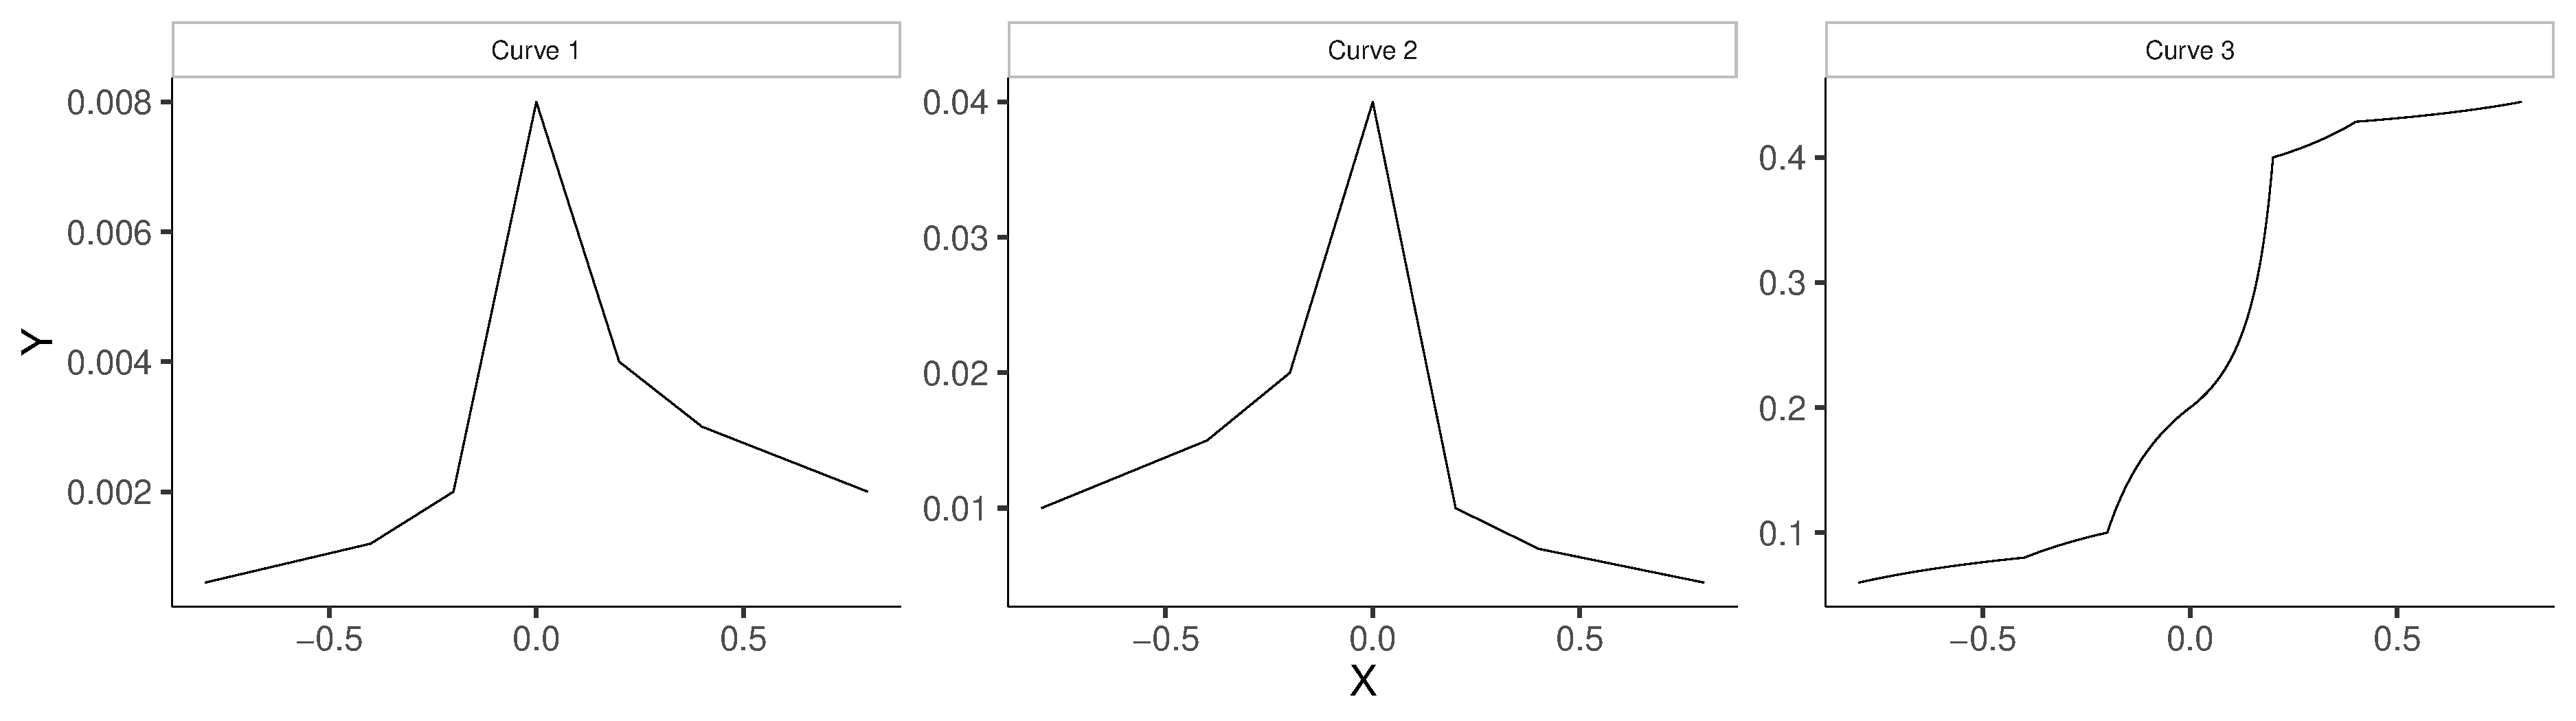
\includegraphics[width=1.1\columnwidth]{illustration.pdf}
	\caption{\small Illustration: An asymmetric inverse  V-shape divided by an oppositely asymmetric inverse V-shape leading to a step-like shape.}
	\label{figure:illustration}
\end{figure}

Table \ref{table:notations} lists notations used in the following discussion.

\begin{table}[H]
	\label{table:notations}
	\caption{Notations}
	\centering
	\small
	\begin{tabular}{l l} 
		\hline
		Variable &\:\:\:\:\:\:\:\:\:\:\:\: Description \\
		\hline
		$N$, $NG$, $NL$ & Number of stocks, gains, and losses in a portfolio, respectively.\\
		Stock $i$ & A stock of interest. \\
		& We are interested in the selling schedule of stock $i$ as a function of\\
		& the return since purchase of stock $i$.\\
		Stock $j$ ($j=${1,2,...N-1})& Stocks other than stock $i$ in the portfolio that stock $i$ belongs to.\\
		$P^{daily}_{i}$ & Daily probability of stock $i$ being sold. \\
		$P^{daily}_{j}$ & Daily probability of stock $j$ being sold. \\
		$P^{sell\mbox{-}day}_{i}$ & Probability of stock $i$ being sold on sell-days.\\
		%$P^{sell-\mbox{-}day}_{j}$ & Probability of stock $j$ being sold on sell-days.\\
		\hline
	\end{tabular}
\end{table}

We will show that a step-like selling schedule on sell-days ($P^{sell\mbox{-}day}_{i}$) is led by a division of two asymmetric inverse V-shaped curves (with convex downward curves both in the gain and the loss domains). To do so, in Section \ref{section:ave}, we first show that $P^{daily}_{i}$ as a function of return since purchase of stock $i$ is asymmetric inverse V-shaped, and then, in Section \ref{section:cond}, we show that the probability of stock $i$ being included in a sell-day portfolio as a function of the return since purchase of stock $i$ is oppositely asymmetric inverse V-shaped. Finally, Section \ref{section:condition} shows the mechanism and conditions where a division of two asymmetric inverse V-shaped curves leads to a step-like curve. 

%\cleardoublepage
\section{Empirical Findings}
\subsection{Data}
In this section, we use stock trading data provided by a large mainstream stockbroker in the UK, which include transaction histories of 182,569 accounts for the period between April 2012 and June 2016. 

Because purchase prices of stocks bought before the beginning of the data period are unknown, accounts opened before the start of the data period were excluded. Multiple intra-day trades conducted on the same account on the same stock were aggregated with quantity weighted prices. Then, we reconstructed daily portfolio data in which each position is recorded everyday from a first purchase date to a liquidation date. Positions opened on the day and short positions were excluded.
The return since purchase was calculated by using a quantity weighted average purchase price of the stock for a given account and a closing price of the stock as of one day prior to the date. Stocks' closing prices were retrieved from the Datastream.\footnote{For stocks' identification in data-merging, we used Stock Exchange Daily Official List (SEDOL) numbers which is used for clearing in the United Kingdom and Ireland.} Commissions and dividends were not considered in the calculation of returns since purchase. Positions having missing variables in either the price data or the transaction data were excluded from the daily portfolio sample.
	
As a consequence, the daily portfolio sample includes 8,573,731 account-days for 20,687 accounts (23,687,688 account-stock-days).


\subsection{The Effect of Weighted-Averaging across Stocks with Different Holding Period}
\label{section:ave}
First, using a small daily portfolio sample consisting of stocks with a holding period no more than 50 days, we illustrate the effect of averaging selling probabilities across stocks which differ in a holding period.

Figure \ref{figure:prop_by_days_less50} shows the daily selling schedule on return since purchase, $P^{daily}_{i}$, separately for five stock groups which differ in holding periods. The curve in each panel is asymmetric V-shaped (i.e., the selling probability increases as an absolute return increases while the positive sensitivity to the absolute return is greater in the gain domain than in the loss domain). In addition, the curve gets flatter as a holding period increases. These are consistent with Figure 1 in \citet{BenDavidHirshleifer12}. The asymmetry of the sensitivity of the selling schedule to the absolute return represents the disposition effect in the daily portfolio sample.

Also, comparing across panels in Figure \ref{figure:prop_by_days_less50}, the selling probability tends to be lower as a holding period increases. That is, the longer the holding period the lower the selling probability.\footnote{The lowest point in the selling schedule in Figure \ref{figure:prop_by_days_less50} is not at zero return but in a region of small losses. This is because the distribution of returns having a highest peak in a region of small losses is used as a weight when averaging selling schedule within stock group. We will discuss the mechanism later. For example, if we use a sample consisting of stocks with a holding period of exactly 1 day, we see the bottom around zero return.} \footnote{The shape may relate to the Ostrich effect as briefly discussed below.} In addition, the reduction of the selling probability on holding period is larger when the holding period is relatively short than when it is long. (Compare, for example, the difference in the selling probability between the leftmost and the second leftmost panels with the difference between the rightmost and the second rightmost panels in Figure \ref{figure:prop_by_days_less50}.)

\begin{figure}[H]
	\centering
	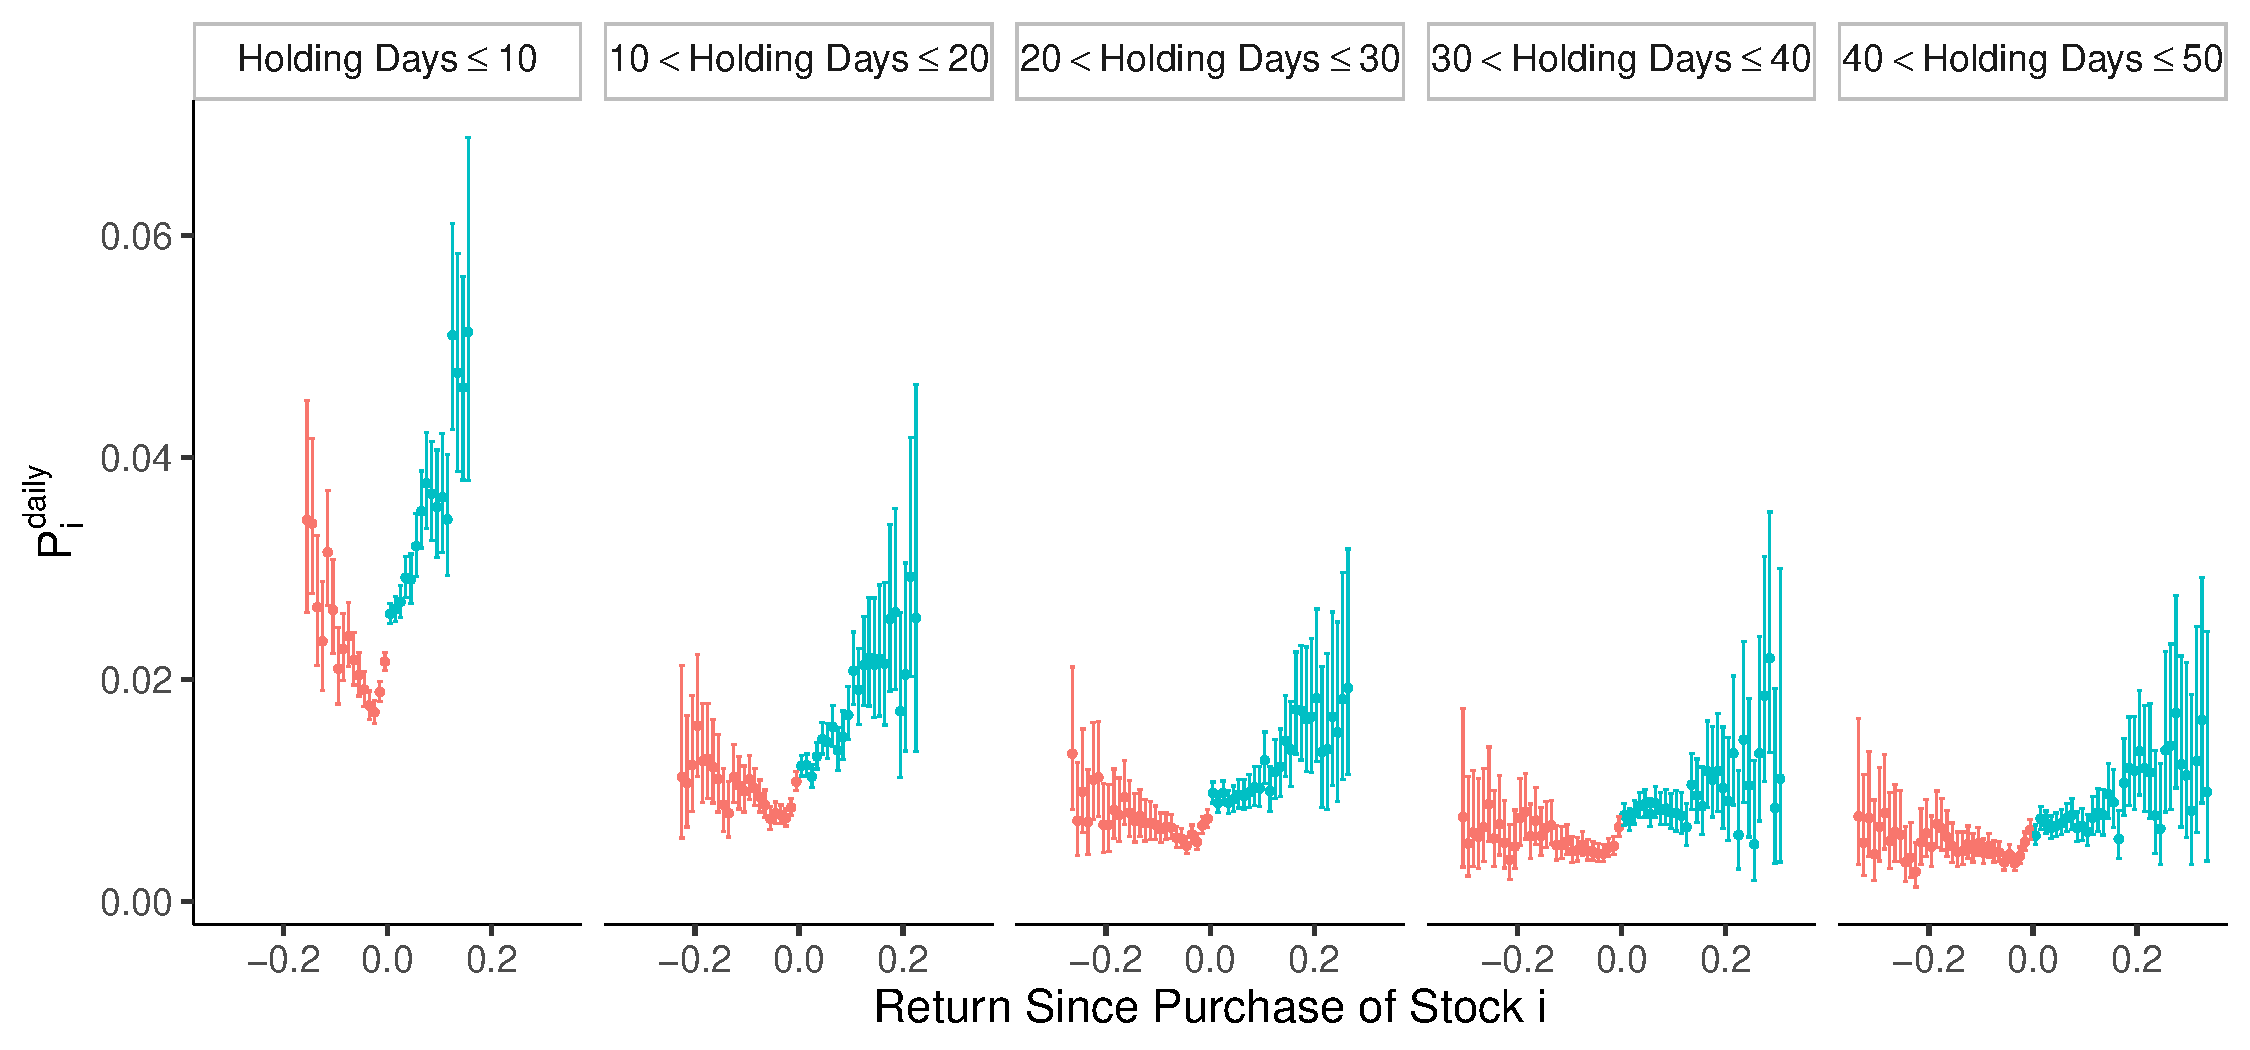
\includegraphics[width=1\columnwidth]{barc_schedule_daily_by_days_less50_3.pdf}
	\caption{\small Proportion of stocks being sold for subsets of stocks by holding days ($P^{daily}_{i}$; Daily portfolio sample consisting of stock with $Holding\mbox{-}days\leq50$). The bin-width is 0.01. The error bars are 95\% confidence intervals.}
	\label{figure:prop_by_days_less50}
\end{figure}

Figure \ref{figure:dist_ret_by_days_less50} plots the distribution of returns since purchase for each of the five stock groups introduced in Figure \ref{figure:prop_by_days_less50}. The shorter the holding period the more the concentration at zero return and the downward curve from the peak at zero return toward either of the positive or the negative domain is mostly convex. These are because of three factors---(i) the larger the absolute return since purchase the larger the selling probability (seen in Figure \ref{figure:prop_by_days_less50}), (ii) the reduction of selling probability is large when the holding period is short (seen in Figure \ref{figure:prop_by_days_less50}), and (iii) mechanically the large the holding period the larger the absolute return.\footnote{Figure \ref{figure:holding_days} shows a relationship between the return since purchase and the holding period.} These three factors together make the reduction of the number of unsold stocks slower as the absolute return increases, leading to the convexity. Note that the distribution of returns since purchase shown in Figure \ref{figure:dist_ret_by_days_less50} reflects the selling schedule shown in Figure \ref{figure:prop_by_days_less50}. 

\begin{figure}[H]
	\centering
	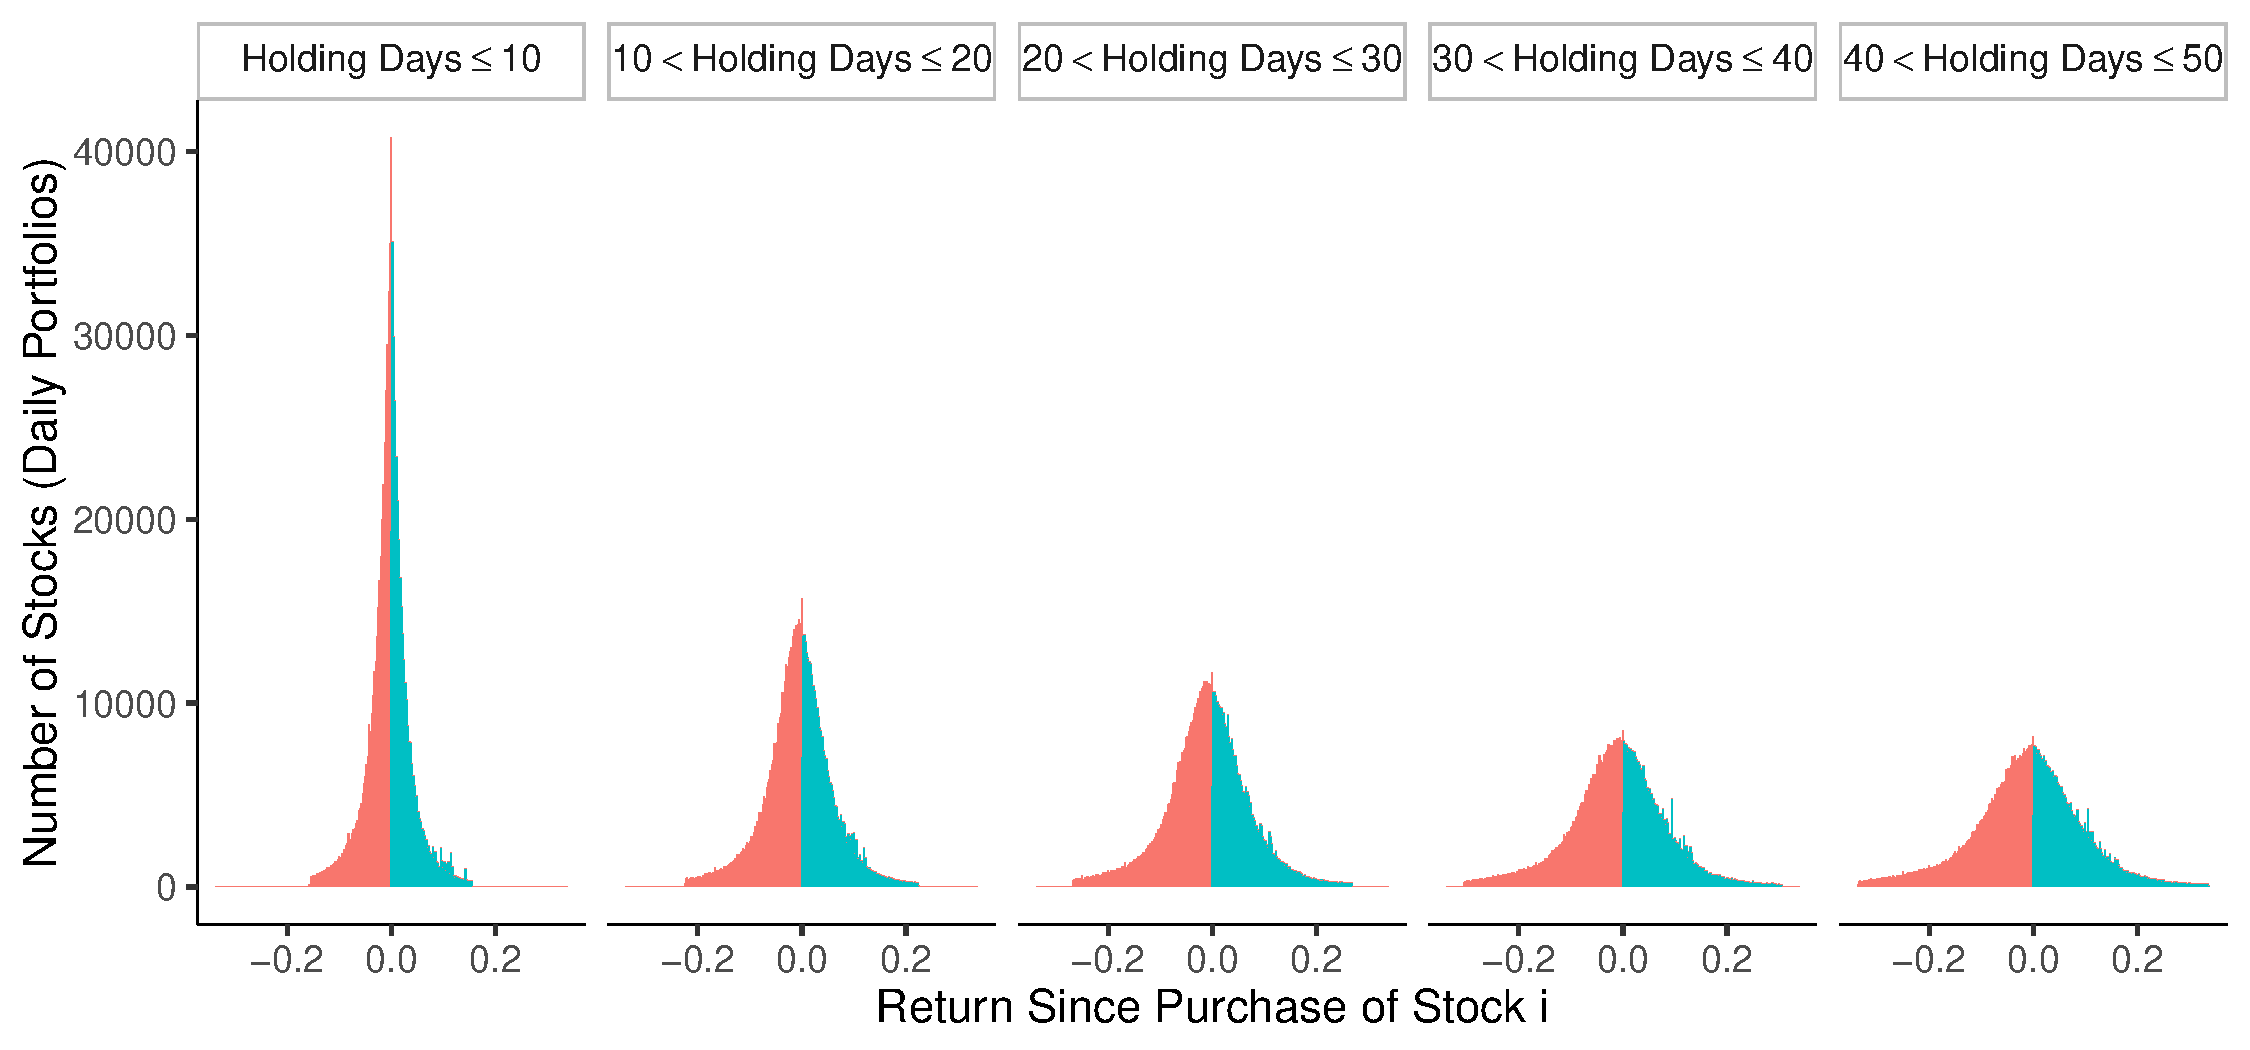
\includegraphics[width=1\columnwidth]{barc_hist_return_daily_less50_3.pdf}
	\caption{\small Distribution of returns since purchase for subsets of stocks by holding days (Daily portfolio sample consisting of stock with $Holding\mbox{-}days\leq50$). The bin-width is 0.25\%.}
	\label{figure:dist_ret_by_days_less50}
\end{figure}


Averaging the selling schedules in Figure \ref{figure:prop_by_days_less50} across stock groups, weighted by the distribution of returns in Figure \ref{figure:dist_ret_by_days_less50} leads to Figure \ref{figure:prop_less50}. 
%The shape of the selling schedule in Figure \ref{figure:prop_less50} is quite different from those in Figure \ref{figure:prop_by_days_less50}.
The selling schedule in Figure \ref{figure:prop_less50} has a peak around zero return. This is because two things work together in the weighted-averaging: (i) As seen in the comparison across panels in Figure \ref{figure:prop_by_days_less50}, stocks with a short holding period has a higher selling probability than stocks with a longer holding period and (ii) As seen in Figure \ref{figure:dist_ret_by_days_less50}, the distribution of returns of the stocks with a short holding period highly concentrates around zero return. 

\begin{figure}[H]
	\centering
	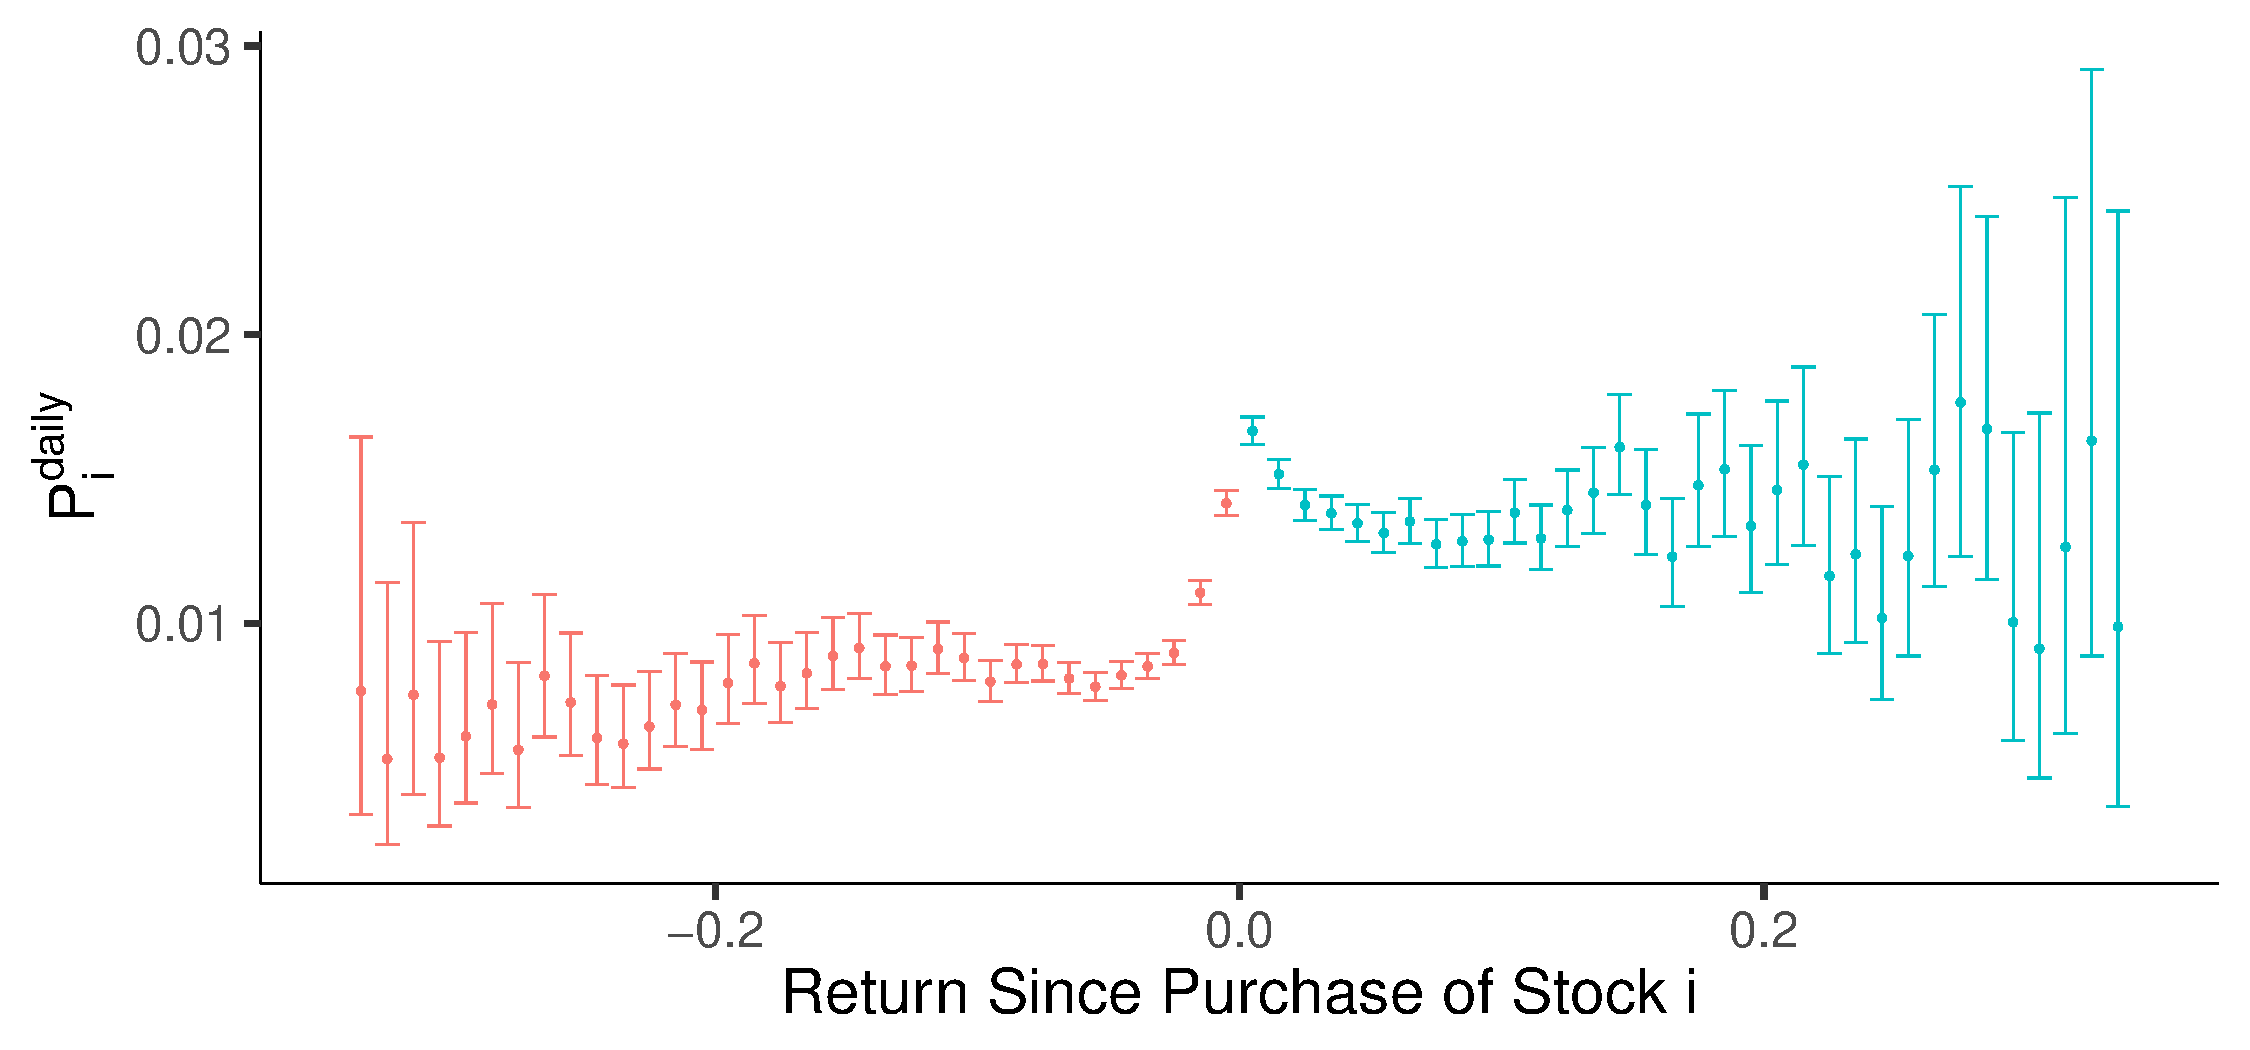
\includegraphics[width=0.8\columnwidth]{barc_schedule_daily_less50_3.pdf}
	\caption{\small Proportion of stocks being sold ($P^{daily}_{i}$; Daily portfolio sample consisting of stock with $Holding\mbox{-}days\leq50$). The bin-width is 0.01. The error bars are 95\% confidence intervals.}
	\label{figure:prop_less50}
\end{figure}


So far, we use the restricted sample including only stocks with a holding period no more than 50 days for illustration purpose.
If we do the weighted-averaging on all daily portfolios\footnote{We use portfolios including at least one gain and at least one loss because the sell-day analysis in studies on the disposition effect examines investors' choice among stocks across domains.}, we have Figure \ref{figure:prop_NG1NL1}. This is the daily selling schedule on return since purchase for all stocks in the daily portfolio sample. 

Similar to Figure \ref{figure:prop_less50}, the aggregated selling probability seen in Figure \ref{figure:prop_NG1NL1} has a high peak at zero return and decreases as an absolute return increases toward either of positive or negative side. This is again because (i) the selling probability decreases as a holding period increases and (ii) the distribution of returns becomes less concentrated at zero return as a holding period increases. (i) and (ii) work together in weighted averaging across stocks with a different holding period, resulting in a high peak at zero return. Also, the downward curve from the peak at zero return seen in Figure \ref{figure:prop_NG1NL1} is convex both in the gain and the loss domains. This is also due to the shape of the distribution of returns since purchase (i.e., the high concentration at zero return and the convex decrease in the selling probability on the absolute return).

In addition, because, as seen  in Figure \ref{figure:prop_by_days_less50}, the positive sensitivity of the selling probability to an absolute return is larger in the gain domain than in the loss domain (i.e.,  V-shape is asymmetric), the downward curve from the peak at zero in Figure \ref{figure:prop_NG1NL1} is steeper in the loss domain than in the gain domain. (We call this shape "asymmetric inverse V-shape".) That is, while the weighted averaging creates a high peak at zero return in aggregated selling schedule, the negative sensitivity of the selling probability to the absolute return is smaller in the gain domain than in the loss domain because, as seen  in Figure \ref{figure:prop_by_days_less50}, the selling probability in each panel increases more in the gain domain than in the loss domain as the absolute return increases.

\begin{figure}[H]
	\centering
	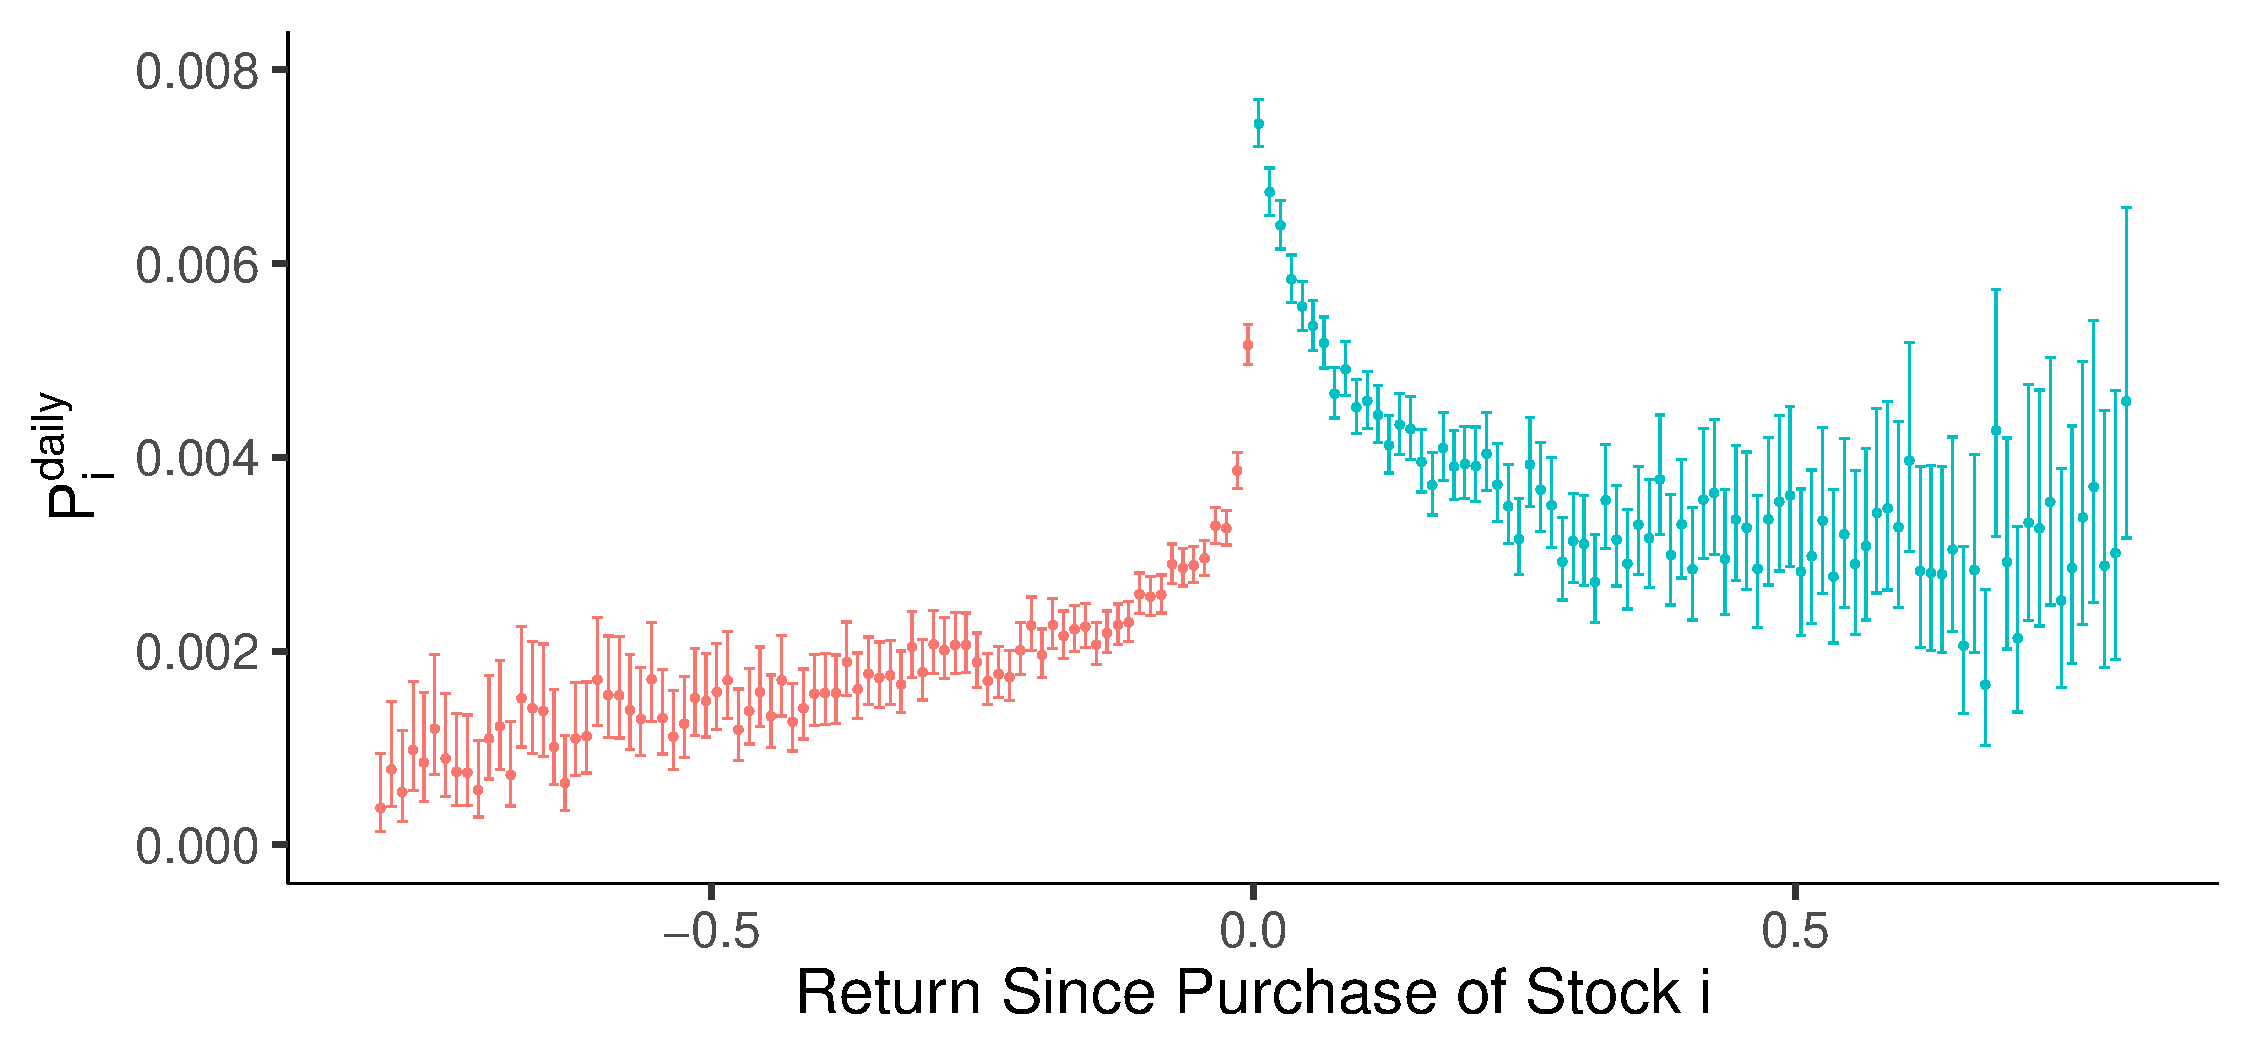
\includegraphics[width=0.8\columnwidth]{barc_schedule_daily_NG1_NL1_3.pdf}
	\caption{Proportion of stocks being sold ($P^{daily}_{i}$; Daily portfolio sample given $NG\geq1$ and $NL\geq1$). The bin-width is 0.01. The error bars are 95\% confidence intervals.}
	\label{figure:prop_NG1NL1}
\end{figure}

\noindent
\textbf{[Interim Summary of Empirical Findings]}\\
As seen in Figure \ref{figure:prop_NG1NL1}, the selling schedule on return since purchase in the daily portfolio sample is asymmetric inverse V-shaped with convex curves both in the gain and the loss domain. This is because the following three factors work together in weighted averaging across stocks with a different holding period.\\

\noindent
(a) The shorter the stock's holding period the higher the daily selling probability of the stock (compare the selling probability across panels in Figure \ref{figure:prop_by_days_less50}).\\
\noindent
(b) The distribution of returns since purchase highly concentrates around zero return and becomes less concentrated as a holding period increases (Figure \ref{figure:dist_ret_by_days_less50}).\\
\noindent
(c) Given a relatively short holding period, the larger the absolute return the higher the daily selling probability while the sensitivity of the selling probability to an absolute return is larger in the gain domain than in the loss domain (asymmetric V-shape in each panel of Figure \ref{figure:prop_by_days_less50}).\\

%Importantly, the steep upward curve toward zero return either from the negative side or the positive side is caused by the high concentration of returns around zero for stocks with a short holding period which, on average, have a high selling probability (Figure \ref{figure:dist_ret_by_days_less50}). 
The factors (a) and (b) lead to the inverse V-shape with convex downward curves in Figure \ref{figure:prop_NG1NL1} and the factor (c) leads to the asymmetry in the sensitivity of the selling schedule to the absolute return (i.e., the asymmetric downward curve from the peak at zero return in Figure \ref{figure:prop_NG1NL1}).\footnote{In other words, even with a completely flat daily selling schedule on return since purchase for a given holding period (i.e., even if the curves in Figure \ref{figure:prop_by_days_less50} were flat), as long as the selling probability decreases as a holding period increases, the weighted-averaging leads to the daily selling schedule on return, averaged across stocks with different holding periods, peaks around zero (i.e., the inverse V-shaped), while the asymmetric V-shaped selling schedule seen in each panel of Figure \ref{figure:prop_by_days_less50} leads to the asymmetry in Figure \ref{figure:prop_NG1NL1}.} 


\subsection{The Effect of Restricting a Sample to Sell-Day Portfolios}
\label{section:cond}

Now we consider the effect of restricting the sample to sell-day portfolios. 

Figure \ref{figure:prop_sell_day_NG1NL1} shows the proportion of stocks in daily portfolios included in a sell-day portfolio (i.e., the probability of stock $i$ being included in a sell-day portfolio as a function of the return since purchase of stock $i$). The curve shape is similar to that in Figure \ref{figure:prop_NG1NL1} (i.e., inverse V-shaped with convex downward curves from the peak). However, as opposed to Figure \ref{figure:prop_NG1NL1}, the downward curve from the peak at zero return is steeper in the gain domain than in the loss domain in Figure \ref{figure:prop_sell_day_NG1NL1}. 


\begin{figure}[H]
	\centering
	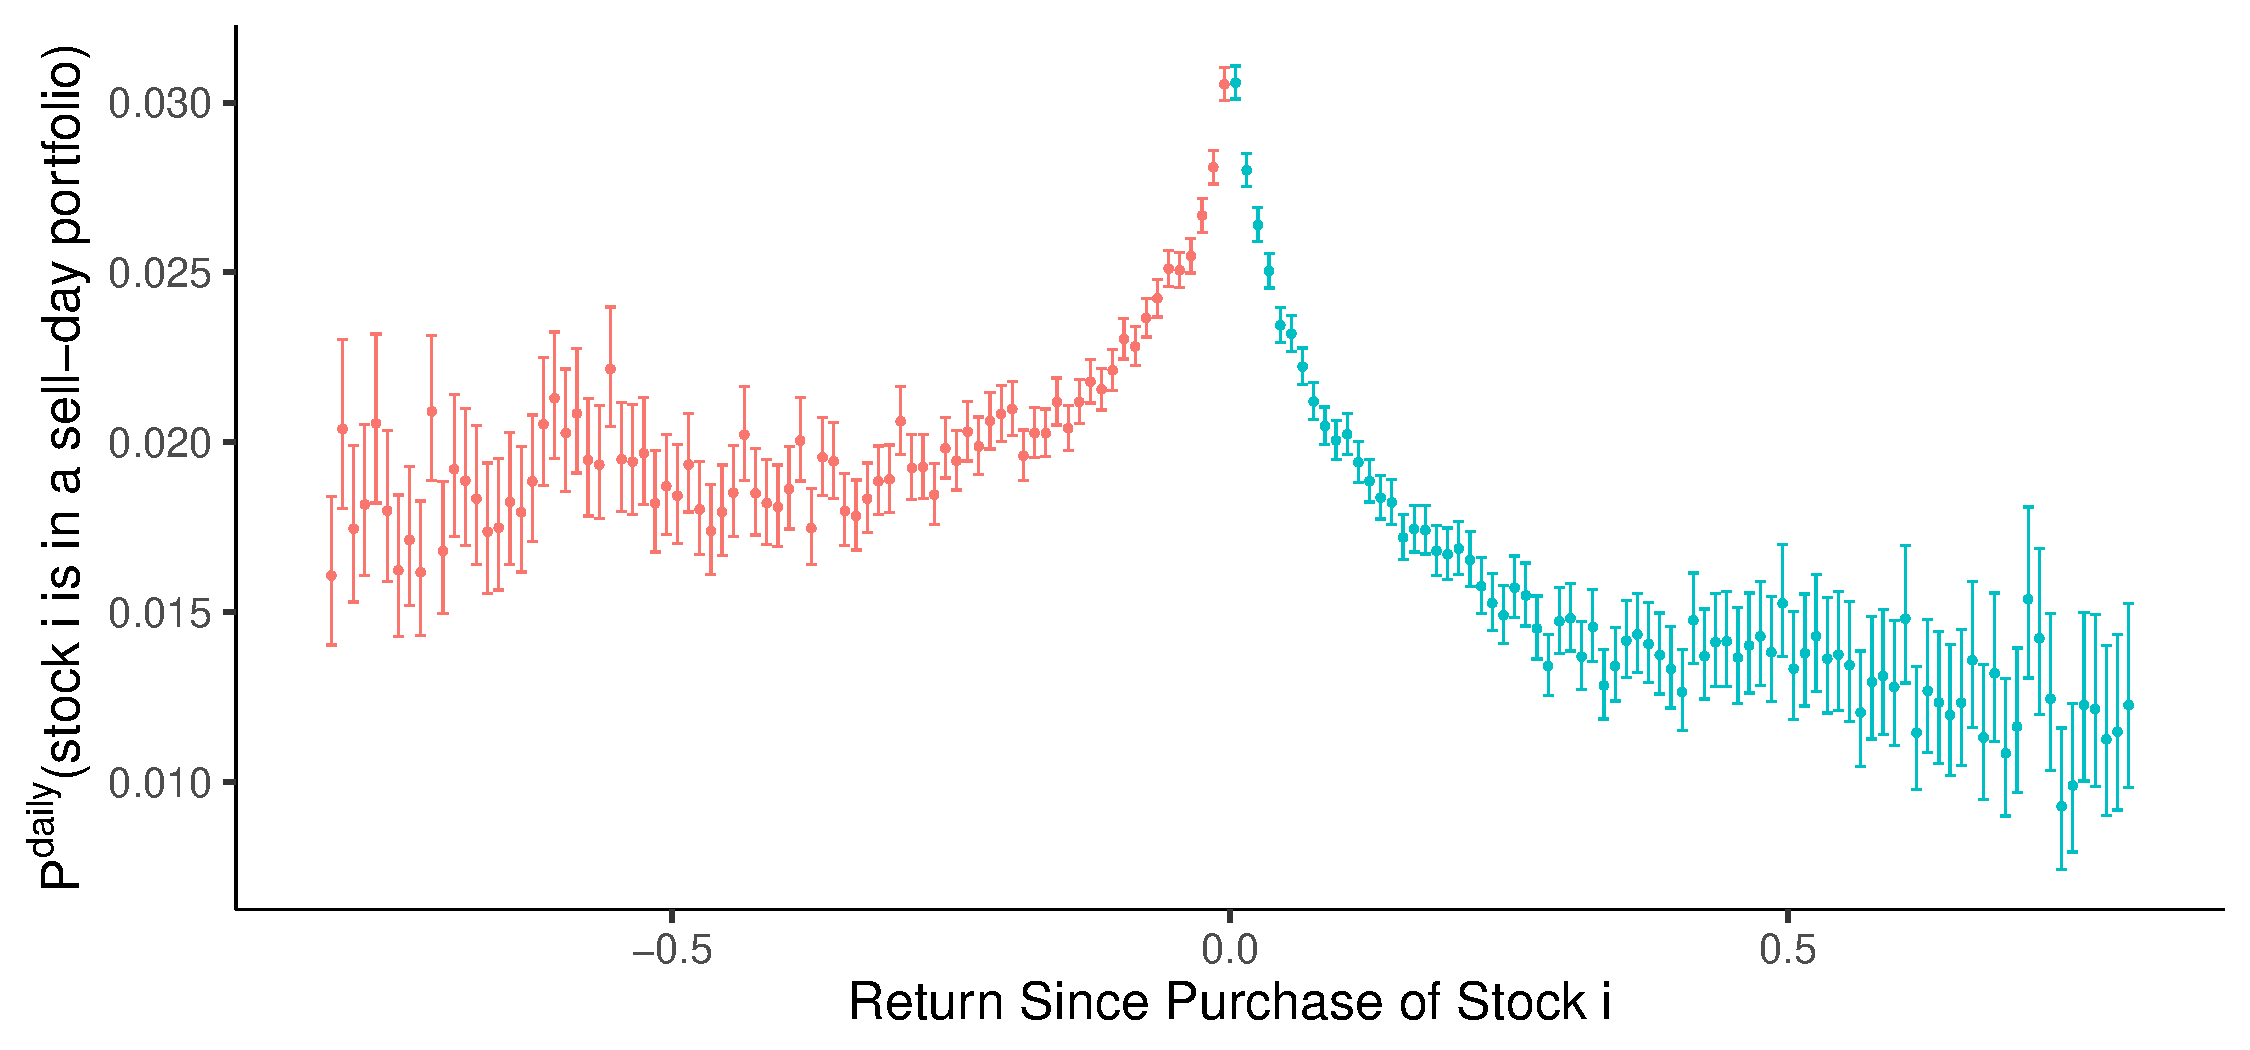
\includegraphics[width=0.8\columnwidth]{barc_port_sell_NG1_NL1_3.pdf}
	\caption{\small Proportion of stocks included in a sell-day portfolio (Daily portfolio sample given $NG\geq1$ and $NL\geq1$). The bin-width is 0.01. The error bars are 95\% confidence intervals.}
	\label{figure:prop_sell_day_NG1NL1}
\end{figure}

As in many previous studies, if we restrict Figure \ref{figure:prop_NG1NL1} to sell-day portfolios, we have the step-like shape seen in Figure \ref{figure:prop_sell_days_NG1NL1}, $P^{sell\mbox{-}day}_{i}$. This is a selling schedule on sell-days.

This sample restriction is equivalent to Figure \ref{figure:prop_NG1NL1}, $P^{daily}_{i}$, divided by Figure \ref{figure:prop_sell_day_NG1NL1}, $P(stock~i~is~in~a~sell\mbox{-}day~portfolio)$. See Equation \ref{eq:1}.\\

\begin{equation}
	\label{eq:1}
P^{sell\mbox{-}day}_{i} = \frac{P^{daily}_{i}}{P(stock~i~is~in~a~sell\mbox{-}day~portfolio)}
\end{equation}
\small
%where $P^{sell\mbox{-}day}_{i}$ is the probability of stock $i$ being sold on sell-days. $P^{daily}_{i}$ is the daily probability of stock $i$ being sold.
%Note that Figure \ref{figure:prop_all} shows $P^{daily}_{i}$ as a function of return of stock $i$. 
%Figure \ref{figure:prop_sell_day} shows $P(Stock~i~is~included~in~a~sell\mbox{-}day~portfolio)$ as a function of return of stock $i$.
%Figure \ref{figure:prop_sell_days} shows $P^{sell\mbox{-}day}_{i}$ as a function of return of stock $i$.\\
\normalsize


\begin{figure}[H]
	\centering
	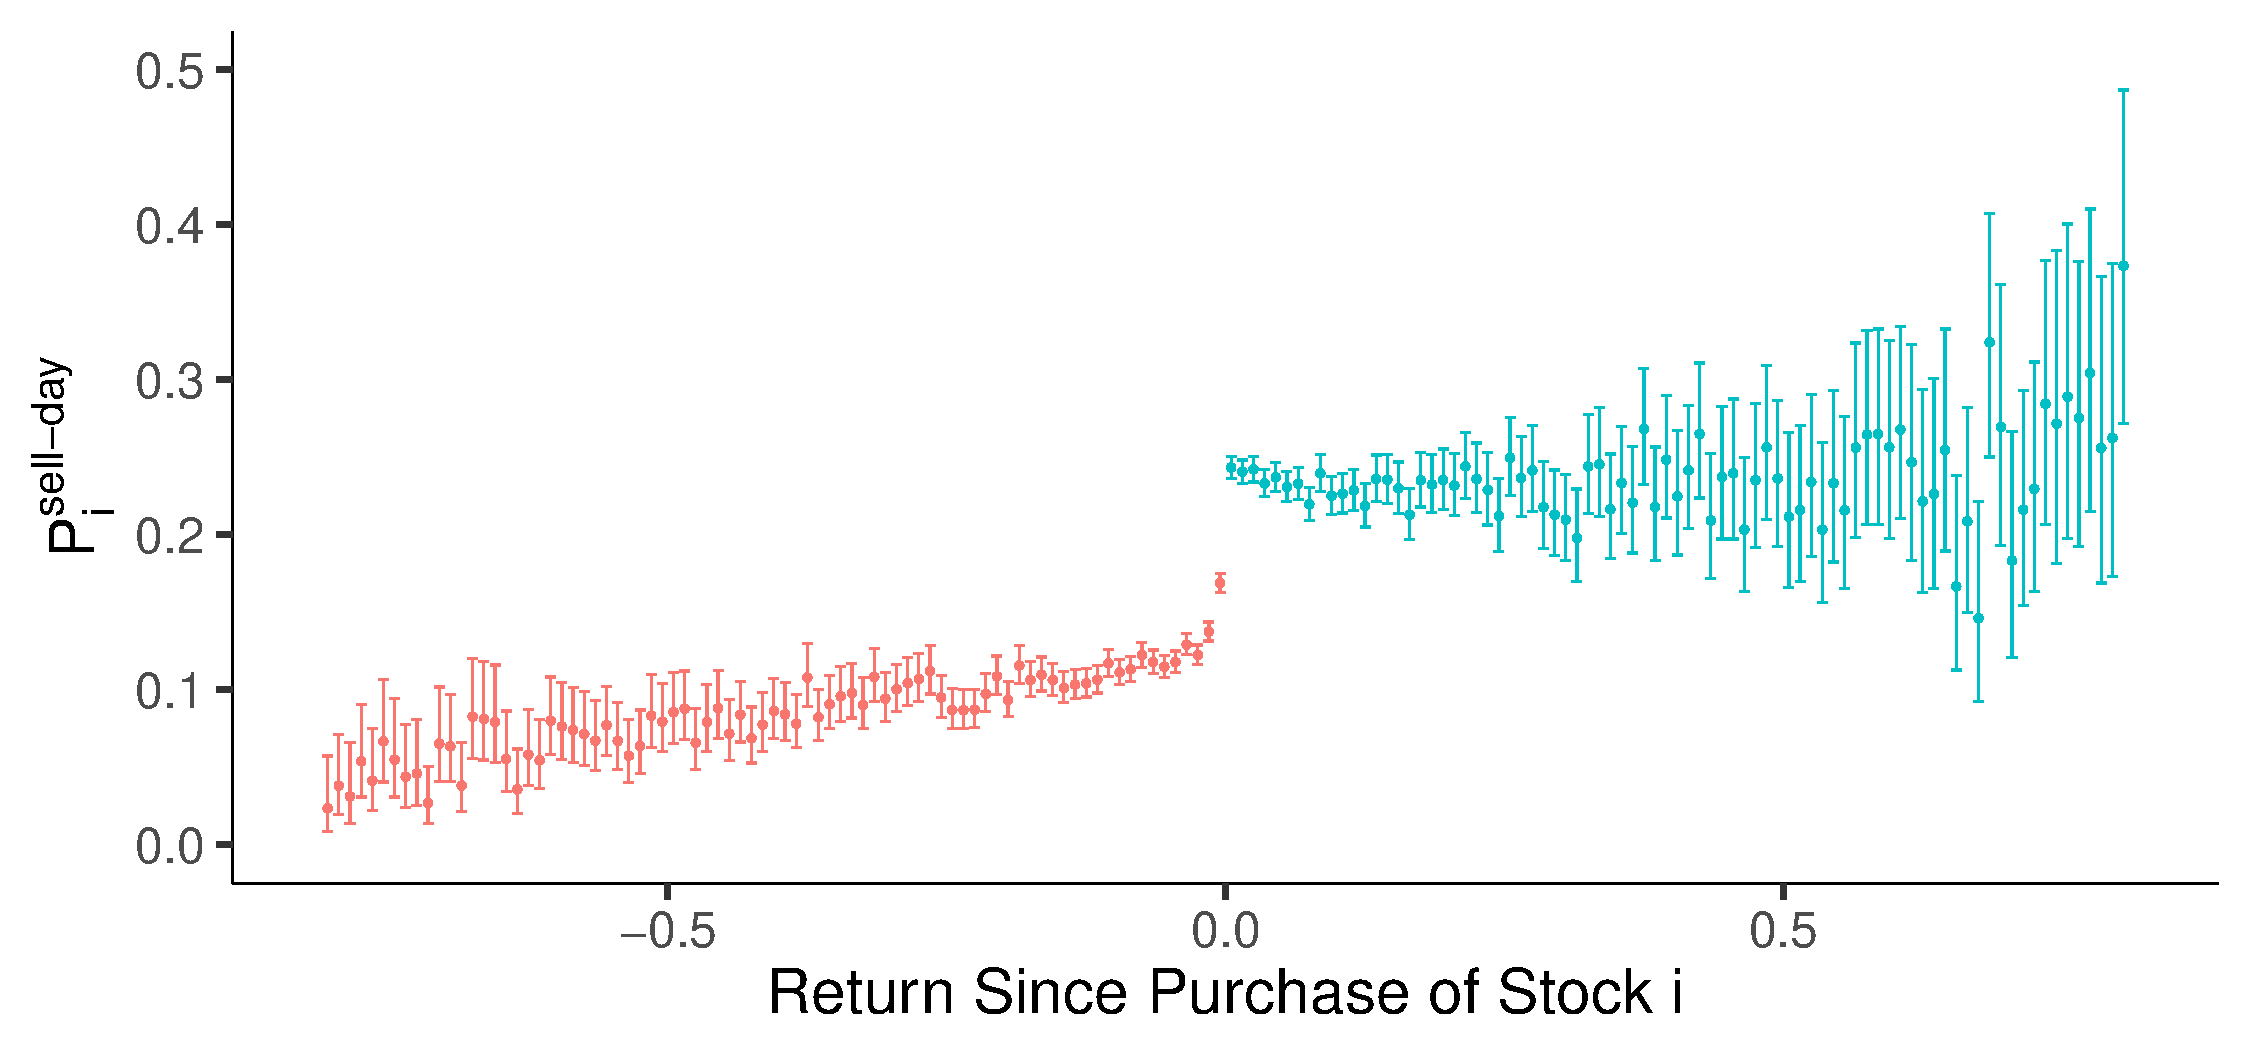
\includegraphics[width=0.8\columnwidth]{barc_schedule_sell_day_NG1_NL1_3.pdf}
	\caption{\small Proportion of stocks being sold ($P^{sell\mbox{-}day}_{i}$; Sell-day portfolio sample given $NG\geq1$ and $NL\geq1$). The bin-width is 0.01. The error bars are 95\% confidence intervals.}
	\label{figure:prop_sell_days_NG1NL1}
\end{figure}

As discussed above, the asymmetric inverse V-shaped daily probability of stock $i$ being sold (Figure \ref{figure:prop_NG1NL1}) divided by the oppositely asymmetric inverse V-shaped probability of stock $i$ being included in a sell-day portfolio (Figure \ref{figure:prop_sell_day_NG1NL1}) leads to the step-like shape (Figure \ref{figure:prop_sell_days_NG1NL1}). (Note that we discuss detailed mechanism about the division of two asymmetric inverse V-shaped curves in Section \ref{section:condition}.) \\

%That is, in the loss domain on the x-axis, the steep curve for $P^{daily}_{i}$ divided by the less steeper curve for $P(stock~i~is~in~a~sell\mbox{-}day~portfolio)$ leads to the further steeper curve  in the neighbor of zero rerurn for $P^{sell\mbox{-}day}_{i}$. On the other hand, in the gain domain, the less steeper curve for $P^{daily}_{i}$ divided by the steeper curve for $P(stock~i~is~in~a~sell\mbox{-}day~portfolio)$ leads to the flatter curve for $P^{sell\mbox{-}day}_{i}$. Two sides together create the step-like shape. 

Then, the next questions are:\\
(1) Why is $P(stock~i~in~a~sell\mbox{-}day~portfolio)$ as a function of return (Figure \ref{figure:prop_sell_day_NG1NL1}) inverse V-shaped?\\
(2) Why is the downward curve from the peak at zero return in Figure \ref{figure:prop_sell_day_NG1NL1} steeper in the gain domain than in the loss domain?\\

%We will answer these two questions one by one. 

$P(stock~i~is~in~a~sell\mbox{-}day~portfolio)$ can be expressed as Equation \ref{eq:2}.%\footnote{Substituting Equation \ref{eq:2} into Equation \ref{eq:1} leads to:
%	\begin{equation*}
%	\label{eq:3}
%	P^{sell\mbox{-}day}_{i} = \frac{P^{daily}_{i}}{1-(1-P^{daily}_{i})\prod_{j=1}^{N-1}(1-P^{daily}_{j})}
%	\end{equation*}
%}

\begin{equation}
\label{eq:2}
P(stock~i~is~in~a~sell\mbox{-}day~portfolio) =1-(1-P^{daily}_{i})\prod_{j=1}^{N-1}(1-P^{daily}_{j})
\end{equation}

Equation \ref{eq:2} indicates that $P(stock~i~is~in~a~sell\mbox{-}day~portfolio)$ increases as the probability of other stocks in the same portfolio being sold, $P^{daily}_{j}$, increases.\footnote{We assume that all of $P^{daily}_{i}$ and $P^{daily}_{j}$ for $j=\{1,2,..N\}$ are independent of each other. Also, $P(stock~i~in~a~sell\mbox{-}day~portfolio)$ increases as the $N$ increases.}\\

If we replace the y-axis of Figure \ref{figure:prop_NG1NL1}, $P^{daily}_{i}$, with $P^{daily}_{j}$, keeping the x-axis variable unchanged, we have Figure \ref{figure:prop_others_NG1NL1}. This is the probability of other stocks (stock $j$) being sold as a function of return of stock $i$.

\begin{figure}[H]
	\centering
	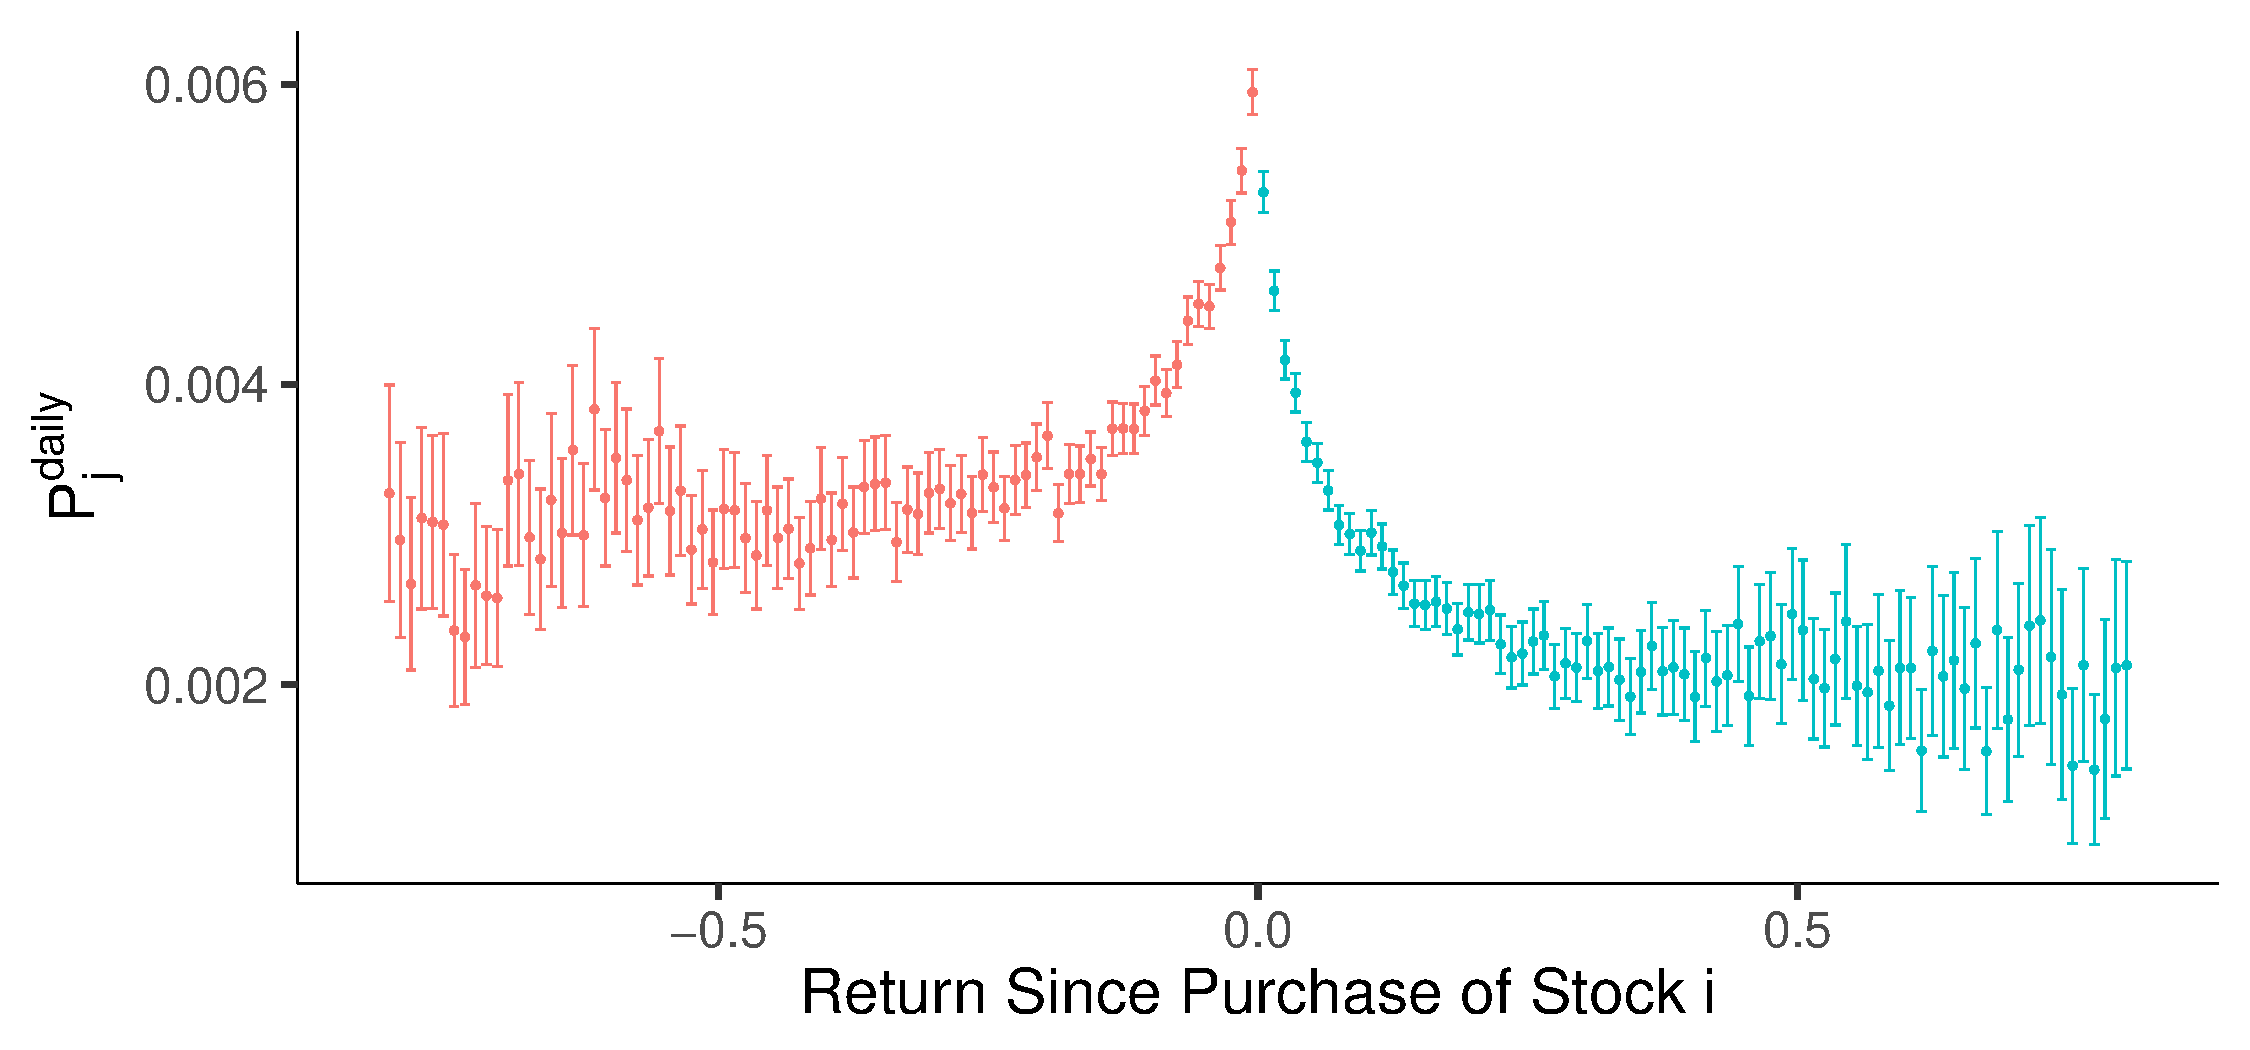
\includegraphics[width=0.8\columnwidth]{barc_other_sold_daily_NG1_NL1_3.pdf}
	\caption{Proportion of other stocks in the portfolios being sold ($P^{daily}_{j}$; Daily portfolio sample given $NG\geq1$ and $NL\geq1$). The bin-width is 0.01. The error bars are 95\% confidence intervals.}
	\label{figure:prop_others_NG1NL1}
\end{figure}

Similar to Figure \ref{figure:prop_NG1NL1}, Figure \ref{figure:prop_others_NG1NL1} is inverse V-shaped. What is a reason of it? 

As seen in Figure \ref{figure:holding_days_i_j_NG1NL1}, the holding period of stock $j$ is, on average, similar to that of stock $i$. Because an absolute return tends to increases as a holding period increases (Figure \ref{figure:holding_days}), the larger the absolute return of stock $i$ the larger the absolute return of stock $j$ (Figure \ref{figure:holding_days_i_j_NG1NL1}). Further, because the selling probability is an increasing function of the absolute return (Figure \ref{figure:holding_days}), the larger the absolute return of stock $i$ the larger the average selling probability of stocks $j$, leading to the inverse V-shape in Figure \ref{figure:prop_others_NG1NL1}. 

%(Note that the downward curves from the peak at zero return in Figure \ref{figure:prop_others_NG1NL1} are convex because the distribution of return since purchase highly concentrates around zero return and stocks with a small absolute return tend to be held together with other stocks with a short holding period associating with a high selling probability.)

In short, $P^{daily}_{j}$ as a function of the return of stock $i$ (Figure \ref{figure:prop_others_NG1NL1}) has a similar shape to $P^{daily}_{i}$ (Figure \ref{figure:prop_NG1NL1}) through the similarity in holding periods among stocks in the same portfolio. 

\begin{figure}[H]
	\centering
	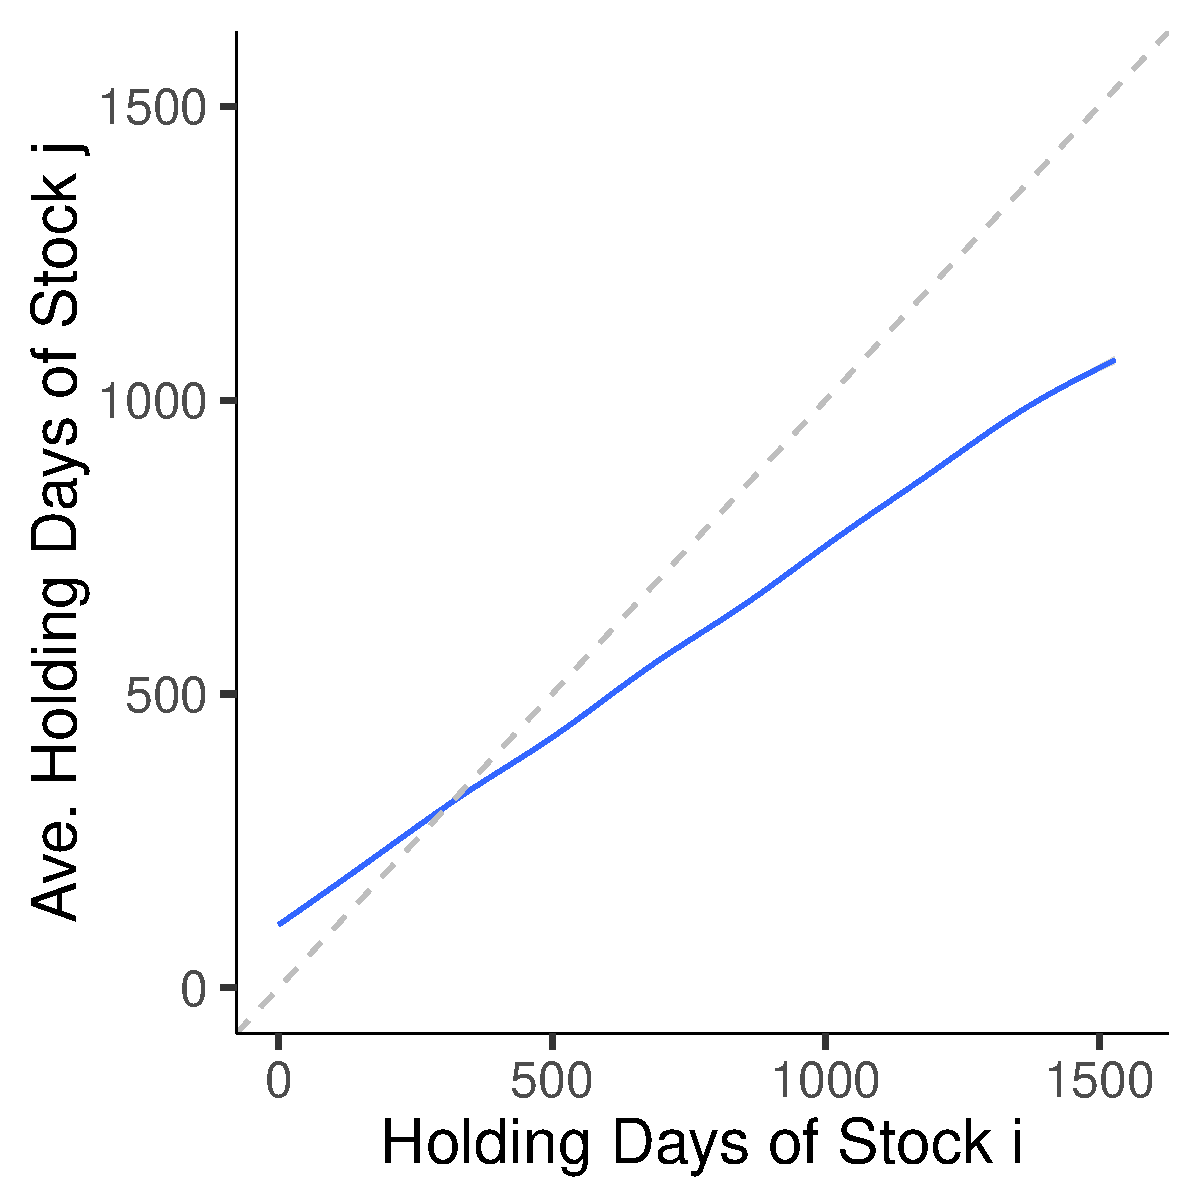
\includegraphics[width=0.5\columnwidth]{barc_holding_days_i_j_NG1_NL1.pdf}
	\caption{Holding Periods of Stock $i$ and Average Holding Period of Stocks $j$.}
	\label{figure:holding_days_i_j_NG1NL1}
\end{figure}


In addition, the downward curve from the peak at zero return in Figure \ref{figure:prop_others_NG1NL1} is steeper when the return of stock $i$ is positive than when the return of stock $i$ is negative. This is because, as seen in Figure \ref{figure:ret_i_abs_j_NG1NL1}, the sensitivity of an absolute return of stock $j$ to an absolute return of stock $i$ is larger when the return of stock $i$ is negative than when the return of stock $i$ is positive. 
That is, because the absolute return of stock $j$ increases more as a return of stock $i$ decreases in the loss domain than as a return of stock $i$ increases in the gain domain (the asymmetric V-shape in Figure \ref{figure:ret_i_abs_j_NG1NL1}), the selling probability of stock $j$ as a function of return of stock $i$, seen in Figure \ref{figure:prop_others_NG1NL1}, deceases less in the loss domain than in the gain domain.
(Remind that the larger the absolute return the larger the selling probability.)  


\begin{figure}[H]
	\centering
	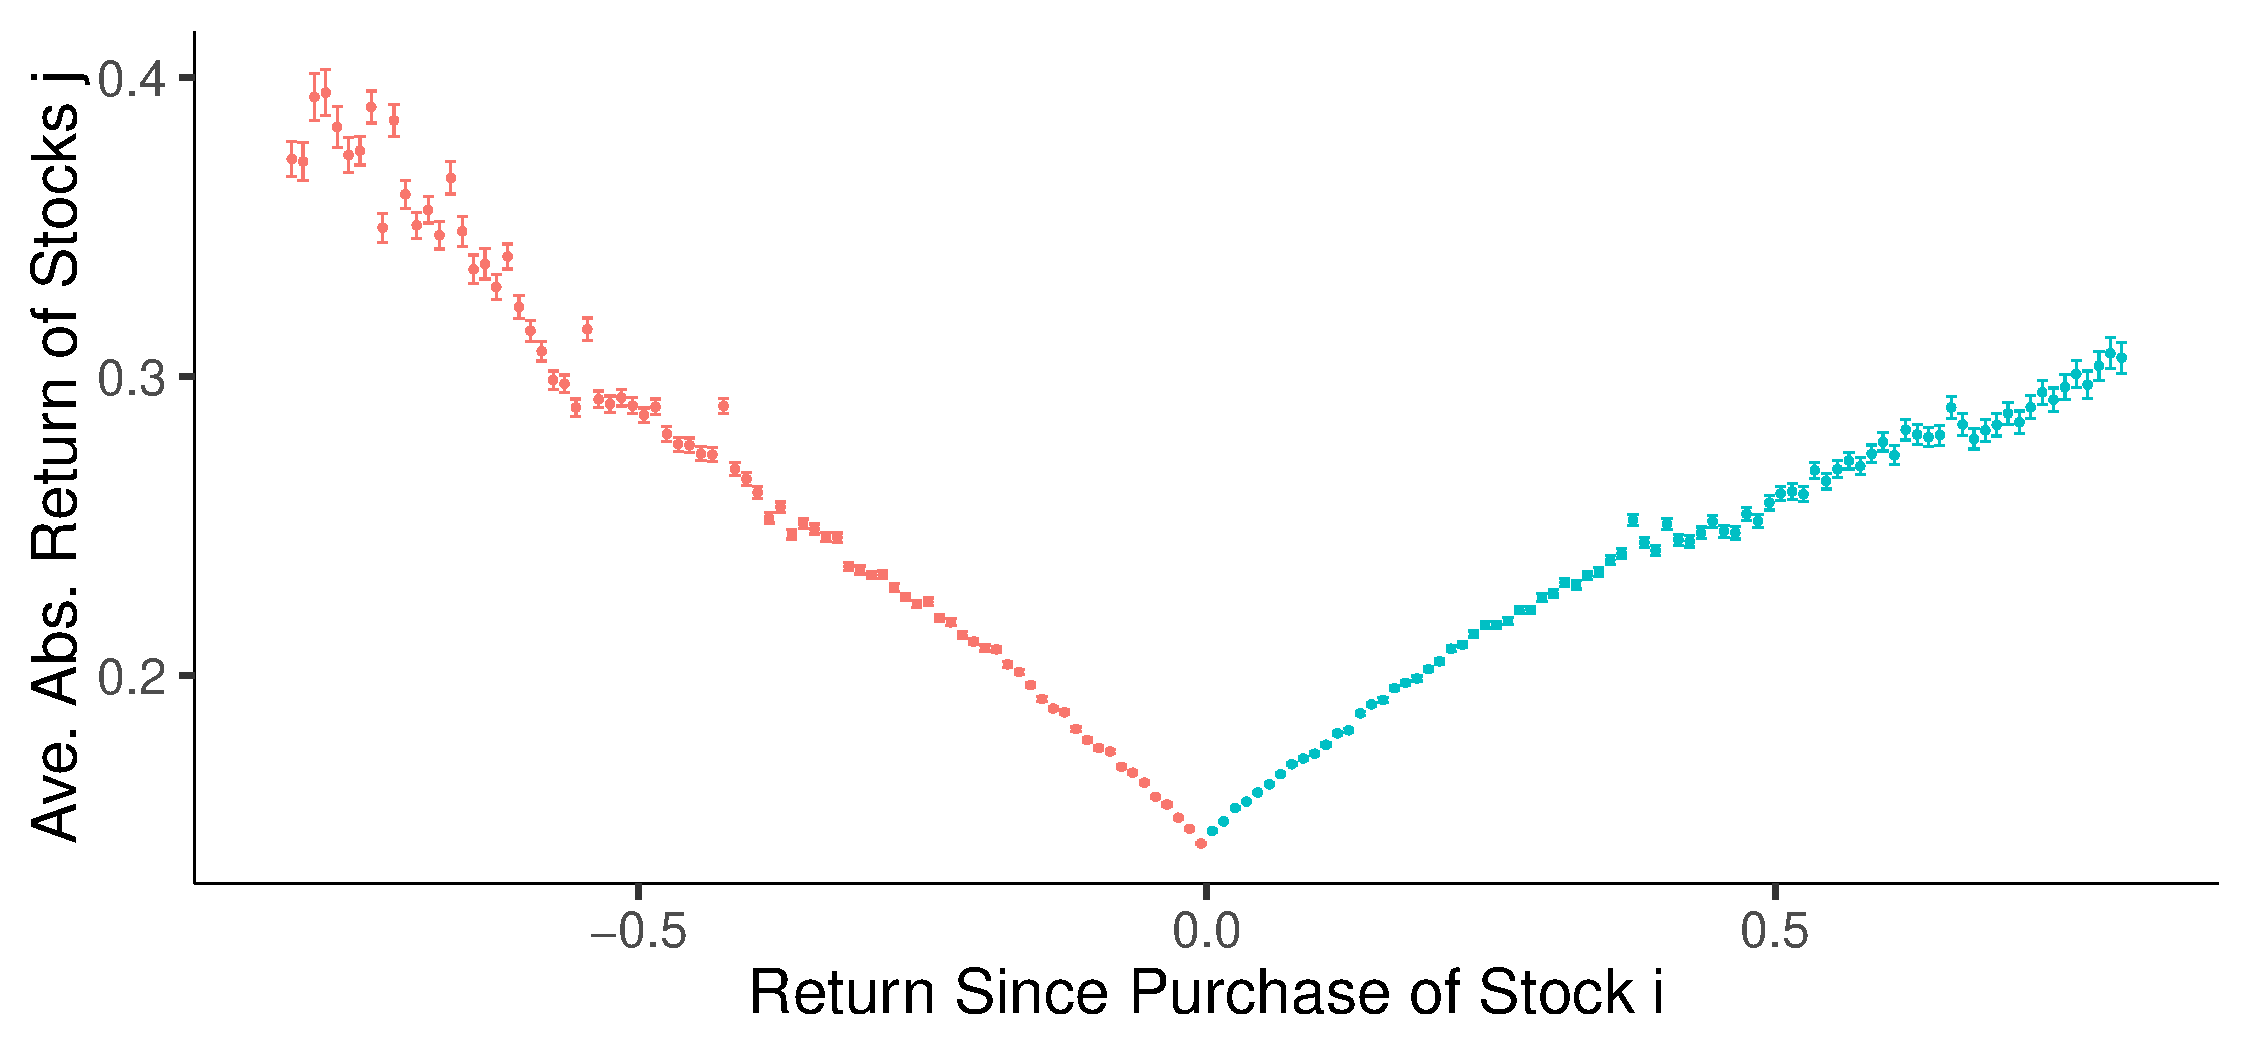
\includegraphics[width=0.8\columnwidth]{barc_R_i_abs_R_j_NG1_NL1.pdf}
	\caption{average absolute return of stocks $j$ as a function of return of stock $i$ (Daily portfolio sample given $NG\geq1$ and $NL\geq1$).}
	\label{figure:ret_i_abs_j_NG1NL1}
\end{figure}


Why is Figure \ref{figure:ret_i_abs_j_NG1NL1} asymmetric? The reason is quite mechanical.

As the return of stock $i$ decreases, stock $i$ tends to have more stocks $j$ having a return larger than that of stock $i$. There is no boundary of stock $j$'s return increasing. Conversely, as the return of stock $i$ increases, stock $i$ tends to have more stocks $j$ having a return smaller than that of stock $i$. However,  stock $j$'s return can decrease only up to -1. Therefore, the sensitivity of the average absolute return of stocks $j$ to the absolute return of stock $i$ becomes asymmetric. 
In short, the curve shape in Figures \ref{figure:prop_others_NG1NL1} and \ref{figure:ret_i_abs_j_NG1NL1} is asymmetric because the distribution of returns since purchase is, by nature, positively skewed. (As Equation \ref{eq:2} tells, Figure \ref{figure:prop_sell_day_NG1NL1} reflects the curve shape in Figure \ref{figure:prop_others_NG1NL1}.)

In order to confirm it, we simulate 1,000-days stock prices following the geometric Brownian motion for 10,000 portfolios, each of which consists of five stocks, and plots an average absolute return of stock $j$ on a return of stock $i$.\footnote{In the same manner as the empirical data, all simulated stocks contribute as stock $i$ once and as stock $j$ four times.} The result shown in Figure \ref{figure:ret_i_abs_j_sim} resembles to the curve shape in Figure \ref{figure:ret_i_abs_j_NG1NL1}. Even simulated stock prices create the asymmetric V-shape in the average absolute return of stock $j$ as a function of return of stock $i$ seen in Figure \ref{figure:ret_i_abs_j_NG1NL1}, indicating that the asymmetry in the average absolute return of stock $j$ as a function of return of stock $i$ is due to mechanical effect (i.e., the positively skewed return distribution).\\

\begin{figure}[H]
	\centering
	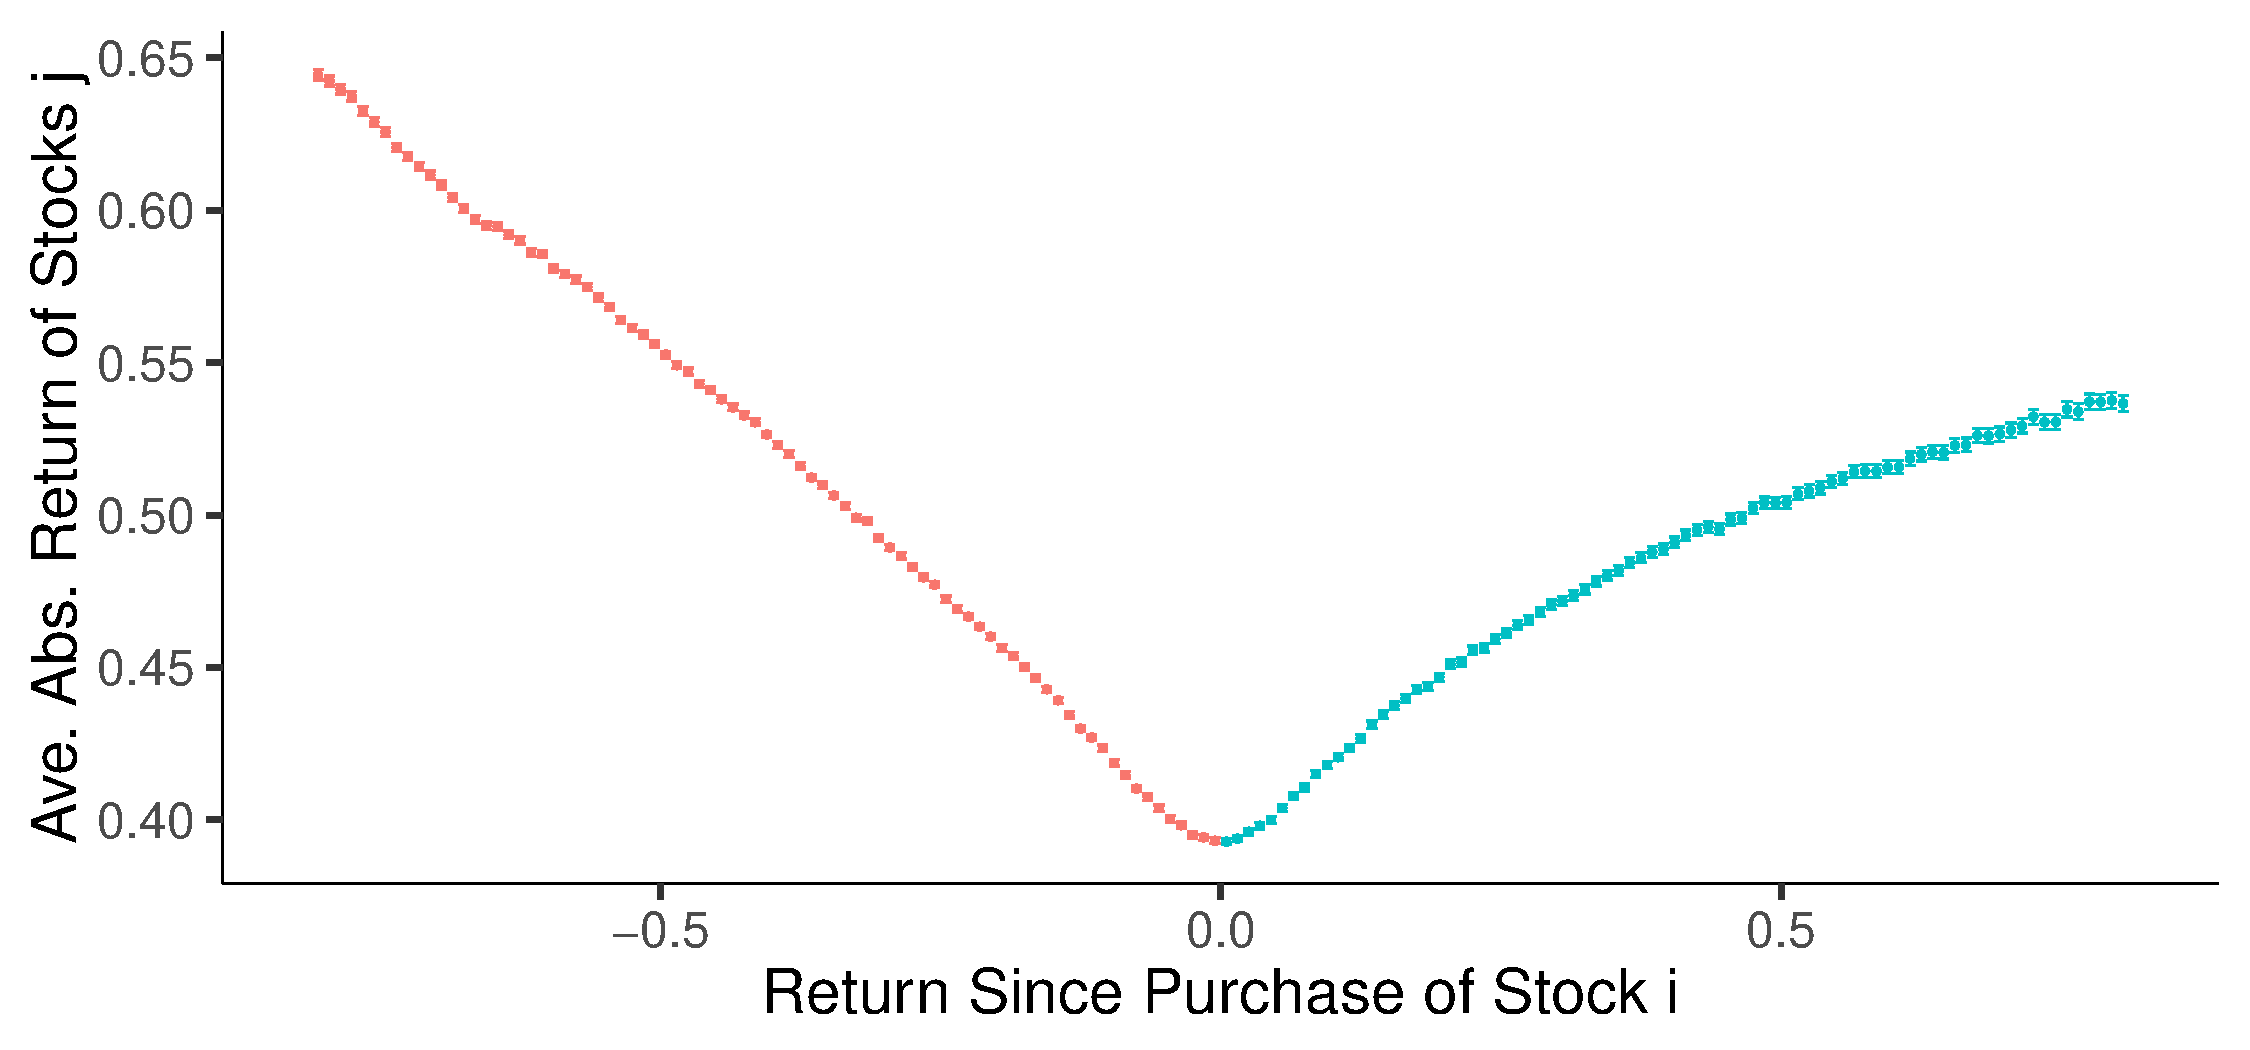
\includegraphics[width=0.8\columnwidth]{sim_R_i_abs_R_j.pdf}
	\caption{Return of stock $i$ and average absolute return of stocks $j$ (Simulated data).}
	\label{figure:ret_i_abs_j_sim}
\end{figure}


Furthermore, P(stock~i~is~in~a~sell\mbox{-}day~portfolio) in Equation \ref{eq:2} can be rewriten as in Equation \ref{eq:3}. 

\begin{equation}
\label{eq:3}
P(stock~i~is~in~a~sell\mbox{-}day~portfolio) = P^{daily}_{i}+(1-P^{daily}_{i})B_2,
\end{equation}
where $B_2$ represents the daily probability of at least one of stocks $j$ being sold: $B_2 = 1-\prod_{j=1}^{N-1}(1-P^{daily}_{j})$. See Appendix \ref{section:more_details} for more details.\\

$B_2$ as a function of the return since purchase of stock $i$, by construction, has a similar shape to that of $P^{daily}_{j}$ seen in Figure \ref{figure:prop_others_NG1NL1}. As discussed above, this is one reason for the oppositely asymmetric inverse V-shape in $P(stock~i~is~in~a~sell\mbox{-}day~portfolio)$ seen in Figure \ref{figure:prop_sell_day_NG1NL1}.
In addition, $(1-P^{daily}_{i})$ which is multiplied to $B_2$ in Equation \ref{eq:3} plays a role to enhance the asymmetry in $B_2$, contributing to the asymmetry of $P(stock~i~is~in~a~sell\mbox{-}day~portfolio)$ which is opposite to the asymmetry of $P^{daily}_{i}$. \\




\noindent
\textbf{[Summary of Empirical Findings]}\\
\noindent
(1) The daily selling schedule on return since purchase, aggregated across stocks, seen in Figure \ref{figure:prop_NG1NL1} is inverse V-shaped with convex downward curves both in the gain and the loss domain. This is because (a) and (b) below work together in the weighted averaging across stocks with a different holding period.\\
\noindent
(a) The shorter the stock's holding period the higher the daily selling probability of the stock. (Compare the selling probability across panels in Figure \ref{figure:prop_by_days_less50}).\\
and\\
\noindent
(b) The distribution of returns since purchase highly concentrates around zero and becomes less concentrated as a holding period increases (Figure \ref{figure:dist_ret_by_days_less50}).\\

\noindent
(2) The negative sensitivity of daily selling schedule to an absolute return seen in Figure \ref{figure:prop_NG1NL1} is larger in the loss domain than in the gain domain because:\\
\noindent
(c) Given a relatively short holding period, the larger the absolute return the higher the daily selling probability while the positive sensitivity of the selling probability to an absolute return is larger in the gain domain than in the loss domain (asymmetric V-shape in each panel of Figure \ref{figure:prop_by_days_less50}). (This asymmetry in the sensitivity represents the disposition effect.)\\

\noindent
(3) The probability of stock $i$ being included in a sell-day portfolio seen in Figure \ref{figure:prop_sell_day_NG1NL1} is inverse V-shaped with convex downward curves from the peak at zero return because:\\
\noindent
(d) Stocks in the same portfolio tend to have a similar holding period (Figure \ref{figure:holding_days_i_j_NG1NL1}).\\
That is, due to the similar holding periods, an absolute return of stock $i$ and that of other stocks in the same portfolio (stocks $j$) are positively correlated, leading to the inverse V-shape in Figure \ref{figure:prop_others_NG1NL1}. This further leads to the inverse V-shape in Figure \ref{figure:prop_sell_day_NG1NL1}. (Refer Equation \ref{eq:2}.)\\

\noindent
(4) The negative sensitivity of the probability of stock $i$ being included in a sell-day portfolio to the absolute return of stock $i$ seen in Figure \ref{figure:prop_sell_day_NG1NL1} is larger in the gain domain than in the loss domain because:\\
\noindent
(e) The distribution of returns since purchase is, by nature, positively skewed with a negative boundary at -1. (Figures \ref{figure:ret_i_abs_j_NG1NL1} and \ref{figure:ret_i_abs_j_sim} show the asymmetric sensitivity of an absolute return of stock $j$ as a function of return of stock $i$.)\\

\noindent
(5) The asymmetric inverse V-shaped curve seen in Figure \ref{figure:prop_NG1NL1} divided by the oppositely asymmetric inverse V-shaped curve seen in Figure \ref{figure:prop_sell_day_NG1NL1} leads to the step-like shape in Figure \ref{figure:prop_sell_days_NG1NL1}. (Note that both Figures  \ref{figure:prop_NG1NL1} and \ref{figure:prop_sell_day_NG1NL1} have convex downward curve in the gain and the loss domains.)\\

%That is, an inverse V-shape (Figure \ref{figure:prop_NG1NL1}) divided by another inverse V-shape (Figure \ref{figure:prop_sell_day_NG1NL1}) makes a resulting curve overall flatter. However, because the numerator (Figure \ref{figure:prop_NG1NL1}) is steeper in the loss domain than in the gain domain, and conversely, the denominator (Figure \ref{figure:prop_sell_day_NG1NL1}) is steeper in the gain domain than in the loss domain, the downward curve from the peak at zero return toward the negative region is preserved while the downward curve toward the positive region becomes flatter. Two sides together creates the step-like shape.\\

Out of five factors listed above, (a) and (c) are behavioral things while (b), (d), and (e) are quite mechanical things.

While "holding period", "absolute return since purchase", and "selling probability" are highly correlated, the causal direction is unknown. For example, stocks with a long holding period may be initially bought with an intention of a long-term investment, leading to the smaller selling probability. Alternatively, investors may pay less attention to stocks as a holding period increases, leading to the smaller selling probability.


The factors (a) and (c) may relate to investors' attention. That is, just after investors buy stocks (or build a portfolio), they pay much attention to their portfolio with a great sensitivity to price movements. However, as a holding period increases, they pay less attention with a less sensitivity to price movements. In addition, due to the ostrich effect, the sensitivity of attention to price movement is greater for stocks in gain than those in loss. 

\section{Details of Division of Two Asymmetric Inverse V-shapes}
\label{section:condition}
Section \ref{section:ave} showed why $P^{daily}_{i}$ as a function of return since purchase of stock $i$ is asymmetric inverse V-shaped. Section \ref{section:cond} showed why $P(stock~i~is~in~a~sell\mbox{-}day~portfolio)$ as a function of return since purchase of stock $i$ is oppositely asymmetric inverse V-shaped (with convex downward curves from a peak at zero return to either of the gain or the loss domain).

In Section \ref{section:division_two_lines}, we review how a division of two lines works, leading to a hyperbola. Then, in Section \ref{section:division_two_inverse_v}, we see the mechanism and conditions where a division of two asymmetric inverse V-shaped probabilities leads to a step-like schedule. Finally, in Section \ref{section:emp_cond}, we see that $P^{daily}_{i}$ as a dividend and\\ $P(stock~i~is~in~a~sell\mbox{-}day~portfolio)$ as a divisor meet those conditions.

\subsection{Mathematics of Division of Two Lines}
\label{section:division_two_lines}
Consider two lines: $y_1=a_1+b_1x$ and $y_2=a_2+b_2x$.\\

\noindent
A division of the two lines is:\\
$y_3 \overset{\underset{\mathrm{def}}{}}{=} \frac{a_1+b_1x}{a_2+b_2x}=\frac{b_1}{b_2}+\frac{a_1-\frac{a_2 b_1}{b_2}}{a_2+b_2x}$\\

\noindent
%A division of the two lines is: $y_3 \overset{\underset{\mathrm{def}}{}}{=} \frac{y_1}{y_2}=\frac{a_1+b_1x}{a_2+b_2x}$.\\

%\noindent
%In the long division format it is: \LongDiv{b_2x+a_2}{b_1x+a_1}\\

%\noindent
%Proceeding a first step in the long division leads to:\\
%$y_3 \overset{\underset{\mathrm{def}}{}}{=} \frac{a_1+b_1x}{a_2+b_2x}=\frac{b_1}{b_2}+\frac{a_1-\frac{a_2 %b_1}{b_2}}{a_2+b_2x}$\\
%($\frac{b_1}{b_2}$ and $a_1{\scriptstyle -}\frac{a_2 b_1}{b_2}$ can be considered as a quotient and a remainder, respectively )\\

\noindent
This means that $y_3$ is a rectangular hyperbola with asymptotes of $x=-\frac{a_2}{b_2}$ (vertical line) and $y=\frac{b_1}{b_2}$ (horizontal line). \\

\noindent
Let $(x_c, y_c)$ denote the center of the rectangular hyperbola: $(x_c, y_c) \overset{\underset{\mathrm{def}}{}}{=} (-\frac{a_2}{b_2}, \frac{b_1}{b_2})$.\\
\noindent
Also, let $A = \frac{a_1-\frac{a_2 b_1}{b_2}}{b_2}$. \\
Then, $y_3= \frac{b_1}{b_2}+\frac{A}{\frac{a_2}{b_2}+x}$.\\

\noindent
This means that the sign of $A$ determines the location of the hyperbola.
That is:\\
The vertices are $(x_c+\sqrt{A}, y_c+\sqrt{A})$ and $(x_c-\sqrt{A}, y_c-\sqrt{A})$. for $A>0$ and\\
The vertices are $(x_c-\sqrt{A}, y_c+\sqrt{A})$ and $(x_c-\sqrt{A}, y_c+\sqrt{A})$. for $A<0$.\footnote{The distance between the center and the vertices is $\sqrt{2A}$. The linear eccentricity is $2\sqrt{A}$ and the eccentricity is $\sqrt{2}$. The radius of curvature at the vertices is $\sqrt{2A}$. Refer https://en.wikipedia.org/wiki/Hyperbola.}\\

%\noindent
%The first term, $\frac{b_1}{b_2}$, represents a vertical shift of the hyperbola.\\
%$a_2$ in the denominator of the second term represents a horizontal shift of the vertical asymptote.\\
%The absolute size of $b_2$ and the absolute size of $a_1-\frac{a_2 b_1}{b_2}$ together determine the eccentricity (i.e., the measure of the curvature) around the vertices. (The larger $|b_2|$ the larger the eccentricity around the vertices.)\\
%The sign of $b_2$ and the sign of $a_1-\frac{a_2 b_1}{b_2}$ together determine quadrants where the hyperbola locates.
%(Note that coordinates axes are asymptotes.)\\
%(Note that the origin of coordinates is the center of the hyperbola.)\\
\noindent
Note that, when $A<0$, the rectangular hyperbola, $y_3$, locates upper-left and lower-right of the center, $(x_c, y_c) = (-\frac{a_2}{b_2}, \frac{b_1}{b_2})$. This means that the hyperbola is upward at any value of $x$. We can confirm it by  taking the first derivative of $y_3$.\\

%\noindent
%$y_3'(x)=\frac{\mbox{-}A}{(\frac{a_2}{b_2}+x)^2}$.\\

\noindent
%As seen above, the first derivative of $y_3$ is:\\
\begin{equation}
\label{eq:deriv}
y_3'(x)=\frac{\mbox{-}A}{(\frac{a_2}{b_2}+x)^2},~where~A = \frac{a_1-\frac{a_2 b_1}{b_2}}{b_2}.
\end{equation}

\noindent
Equation \ref{eq:deriv} indicates that:\\ 
(1) $y_3$ is upward anywhere when $A<0$.\\
(2) $y_3$ gets flatter as the distance between $x$ and the vertical asymptote $\mbox{-}\frac{a_2}{b_2}$ increases.\\
(3) $y_3$ gets flatter as the difference between $\frac{b_1}{a_1}$ and $\frac{b_2}{a_2}$ decreases.\\% (for a given $b_2$).\\
%(3) as $b_2$ decreases (for given $a_1$, $a_2$, and $b_1$).\\

\noindent
In sum, as long as $A<0$, the slope (i.e., the first derivative line) is always positive. The steepness of the slope is determined by the distance between $x$ and the vertical asymptote, $\mbox{-}\frac{a_2}{b_2}$ (the denominator) and the size of $A$ (the numerator).\\

\subsection{Division of Two Asymmetric Inverse V-shaped Probabilities}
\label{section:division_two_inverse_v}

Now we approximate an asymmetric inverse V-shaped curves as a joint of many lines. Continuing the above notations and consider that:\\
$x$ is a small range of return since purchase of stock $i$,\\
$y_1$ is $p^{daily}_{i}$ for the range of $x$,\\
$y_2$ is $P(stock~i~is~in~a~sell\mbox{-}day~portfolio)$ for the range of $x$, and \\
$y_3$ is $P^{sell\mbox{-}day}_{i}$ for the range of $x$. \\

\noindent
Note that, by construction, $y_2$ is always larger than $y_1$ (i.e., $y_2>y_1$ for $N \geq2$). This leads to $a_2>a_1$.\\

\noindent
In this illustrative example, as seen in the left and the middle panels in Figure \ref{figure:illustration_color}, we approximate the upward curve in the negative domain with three lines and the downward curve in the positive domain with three lines. In each domain, the line is steeper around $x=0$ and gets flatter as $|x|$ increases (i.e., convex).\\

\noindent
First, we consider when $y_3$ is upward.\\ 
As seen in Equation \ref{eq:deriv}, when $A<0$, $y_3$ is upward.\\

\noindent
In the negative domain, $b_1>0$ and $b_2>0$.\\
Thus $A = \frac{a_1-\frac{a_2 b_1}{b_2}}{b_2}<0$ is satisfied only when  $\frac{b_2}{a_2} < \frac{b_1}{a_1}$.\\

\noindent
Conversely, in the positive domain, $b_1<0$ and $b_2<0$.\\
Thus, $A = \frac{a_1-\frac{a_2 b_1}{b_2}}{b_2}<0$ is satisfied only when $\frac{b_2}{a_2} < \frac{b_1}{a_1}$.\\

\noindent
Therefore, regardless of a value of $x$, the condition to make $y_3$ upward is $\frac{b_2}{a_2} < \frac{b_1}{a_1}$  (Condition 1).\\

\noindent
When Condition 1 is met, the rectangular hyperbola, $y_3$, locates upper-left and lower-right of the center, $(x_c, y_c) = (-\frac{a_2}{b_2}, \frac{b_1}{b_2})$, and thus, is upward anywhere.\\

\noindent
In addition, because $y_2$ is a probability, it should not be negative. Therefore, in the loss domain, $x$ should be greater than the x-intercept of $y_2$, $-\frac{a_2}{b_2}$, which is the vertical asymptote of the hyperbola. Thus when Condition 1 is met for $x<0$, the corresponding $y_3$ locates lower-right of the center.
Similarly, in the gain domain, $x$ should be less than the x-intercept of $y_2$, $-\frac{a_2}{b_2}$, which is vertical asymptote of the hyperbola. Thus when Condition 1 is met for $x>0$, the corresponding $y_3$ locates upper-left of the center.\\ 

%\noindent
%In the negative domain, $b_1>0$ and $b_2>0$.\\
%Therefore, $A = \frac{a_1-\frac{a_2 b_1}{b_2}}{b_2}$ is negative only when $\frac{b_2}{a_2} < \frac{b_1}{a_1}$ (Condition 1).\\
%Condition 1 means that, when separately plotting $y_1$ and $y_2$ for $x<0$ with a free y-scale ranging from 0 to $a_1$ or $a_2$, the slope of the line is visually steeper for $y_1$ than for $y_2$.\\

%\noindent
%When Condition 1 is met, $A<0$. Then, the rectangular hyperbola, $y_3$, locates upper-left and lower-right of the center, $(x_c, y_c) = (-\frac{a_2}{b_2}, \frac{b_1}{b_2})$, and thus, is upward anywhere.\\ 

%\noindent
%In addition, because $y_2 \geq 0$ and $b_2>0$, $x$ should be greater than the vertical asymptote, $-\frac{a_2}{b_2}$. (I.e., Because $y_2$ is a probability, it should not be negative.) Thus, when Condition 1 is met, corresponding $y_3$ locates lower-right of the center. \\

%\noindent
%Conversely, in the positive domain, $b_1<0$ and $b_2<0$.\\
%Therefore, $A = \frac{a_1-\frac{a_2 b_1}{b_2}}{b_2}$ is negative only when $\frac{b_2}{a_2} < \frac{b_1}{a_1}$ (Condition 2). Note that the inequality is the same to Condition 1. However, as opposed to Condition 1, the sign of $b_1$ and $b_2$ are negative\\
%Condition 2 means that, when separately plotting $y_1$ and $y_2$ for $x>0$ with a free y-scale ranging from 0 to $a_1$ or $a_2$, the slope of the line is visually negatively steeper for $y_2$ than for $y_1$.\\

%\noindent
%When Condition 2 is met, $A<0$. Then, the rectangular hyperbola, $y_3$, locates upper-left and lower-right of the center, $(x_c, y_c) = (-\frac{a_2}{b_2}, \frac{b_1}{b_2})$, and thus, is upward anywhere.\\ 

%\noindent
%In addition, because $y_2 \geq 0$ and $b_2<0$, $x$ should be less than the vertical asymptote, $-\frac{a_2}{b_2}$. Thus, when Condition 2 is met, corresponding $y_3$ locates upper-left of the center. \\

\noindent
A division of two lines resulting in a part of a rectangular hyperbola is illustrated in Figure \ref{figure:illustration_hyperbola}. In each column, the blue line divided by the red line in the top panel results in the colored part of the hyperbola in the bottom panel. The colored part in the bottom panels corresponds to the same-colored curve in the right panel of Figure \ref{figure:illustration_color}.

\begin{figure}[H]
	\centering
	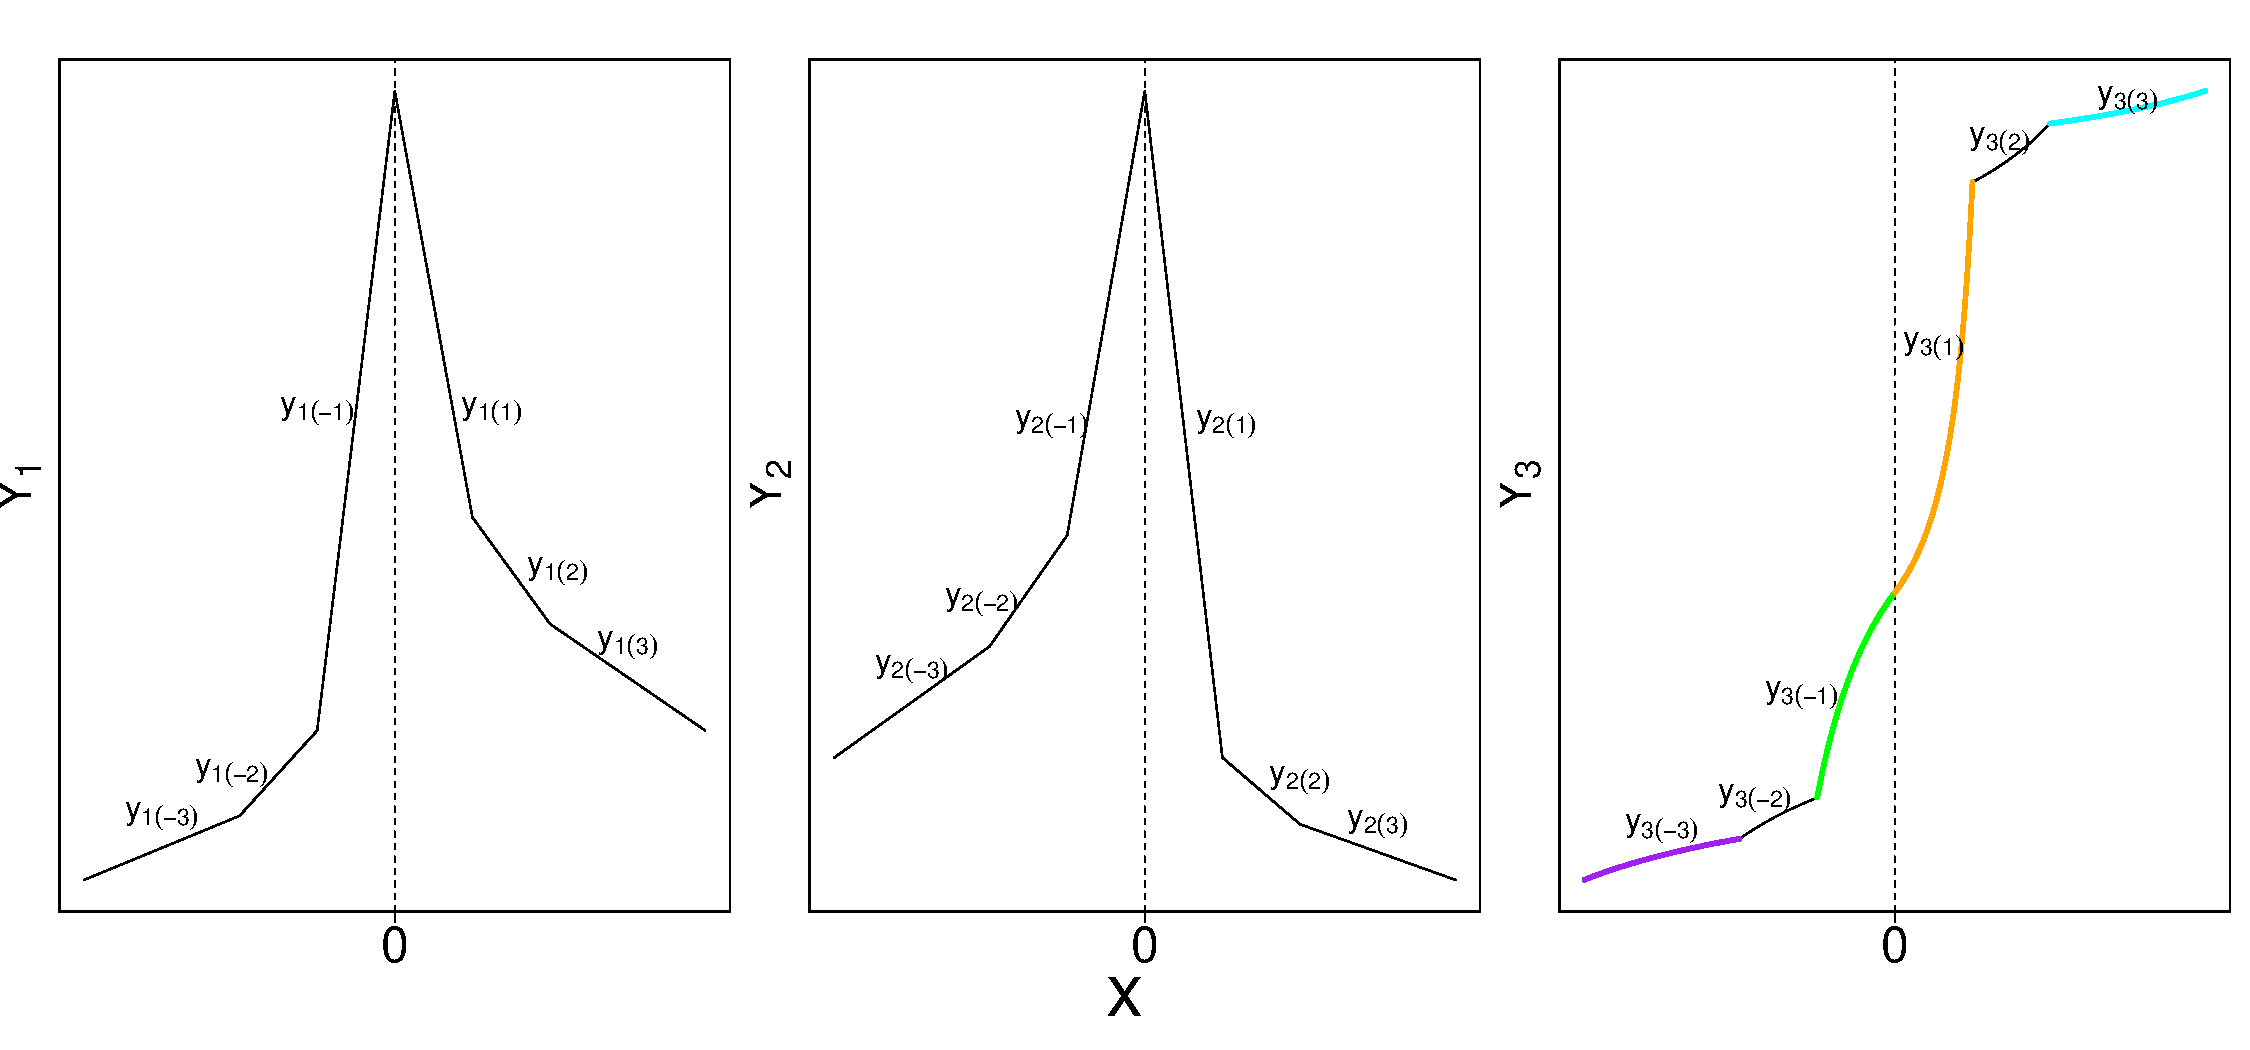
\includegraphics[width=0.9\columnwidth]{illustration_color.pdf}
	\caption{\small Illustration: An asymmetric inverse V-shape divided by an oppositely asymmetric inverse V-shape leading to a step-like shape. The colored parts in the right panel corresponds to the same-colored parts in the bottom panels of Figure \ref{figure:illustration_hyperbola}.}
	\label{figure:illustration_color}
\end{figure}


\begin{figure}[H]
	\centering
	\hspace*{-2cm} 
	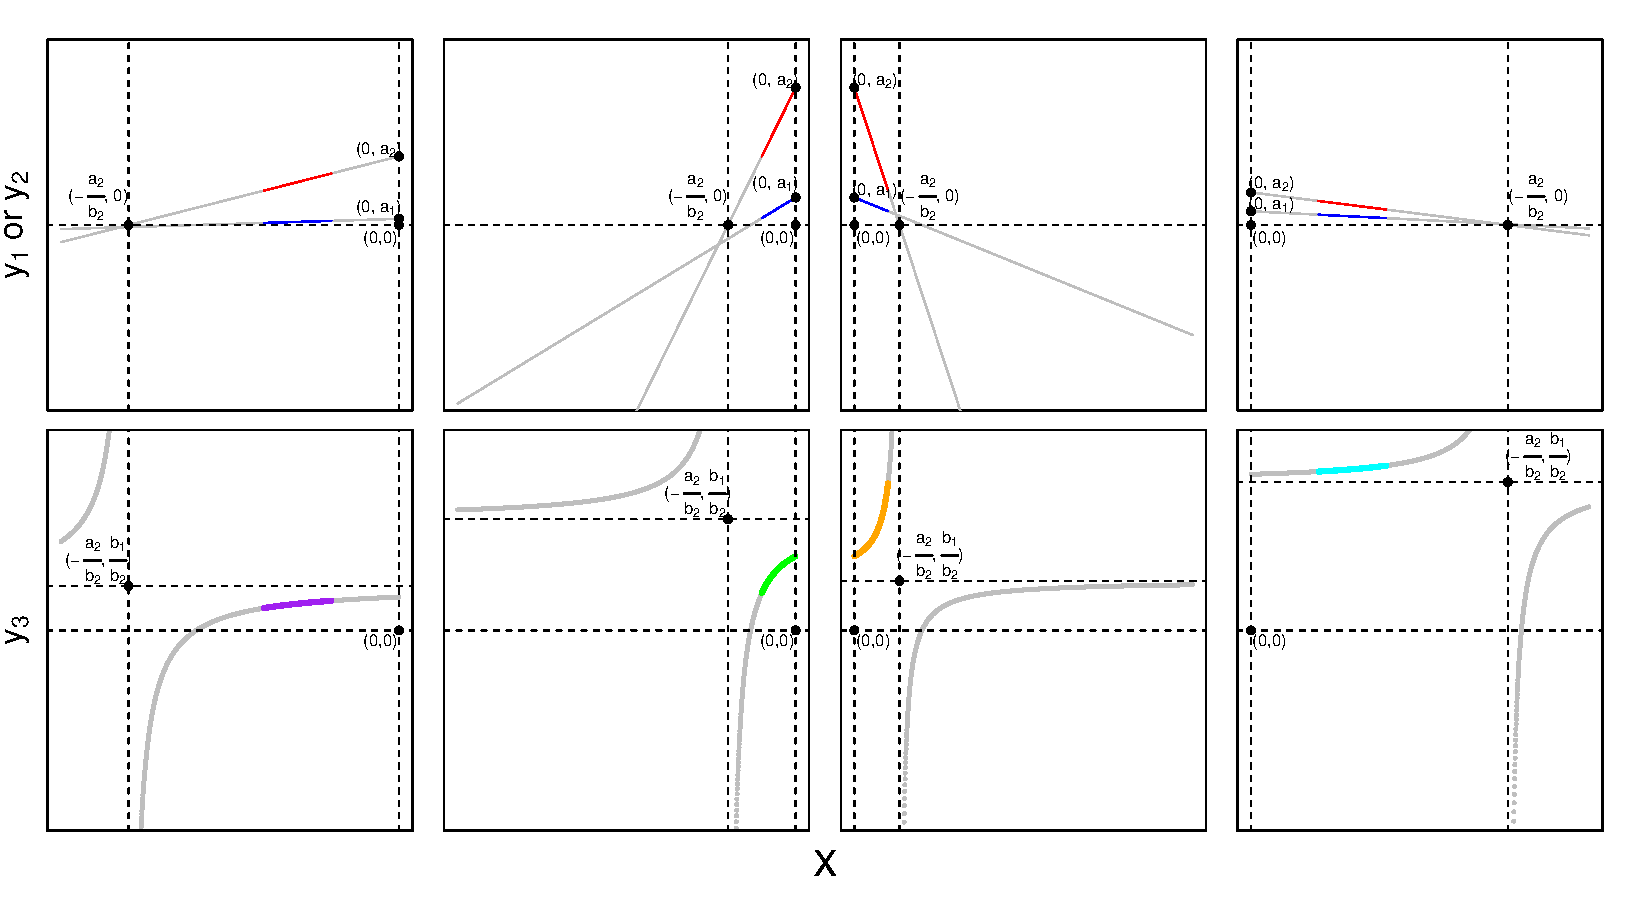
\includegraphics[width=1.4\columnwidth]{illustration_together.pdf}
	\caption{\small Illustration: Division of two asymmetric inverse V-shaped curve approximated as a joint of many lines. The blue line divided by the red line in the top panels leads to the colored parts of the curve in the bottom panels. The colored parts in the bottom panels corresponds to the same-colored parts in the right panel of Figure \ref{figure:illustration_color}.}
	\label{figure:illustration_hyperbola}
\end{figure}

%\noindent
%The discussion above shows that the curve of $y_3$ is upward because it is a part of a rectangular hyperbola with a negative $A$ (thus locating in the first and the fourth quadrant in a coordinate having an origin at the center of the hyperbola). However, in the negative domain of Figure \ref{figure:illustration_hyperbola}, the green curve is much steeper than the purple curve, and similarly, in the positive domain, the orange curve is much steeper than the light-blue curve. What is a reason behind it?\\

%\noindent
%The convex downward curves of $y_2$ from the peak at $x=0$ to either of negative or positive side (the middle panel of  Figure \ref{figure:illustration_color}) means that $-\frac{a_2}{b_2}$ (i.e., the x-intercept of each line) gets larger in an absolute term as $|x|$ increases. Therefore, in the negative domain, the vertical asymptote, $y=-\frac{a_2}{b_2}$, gets more far from the origin, $(x, y)=(0, 0)$, as $x$ gets more negative, and thus, the corresponding part of the hyperbola is likely to be flatter as $x$ decreases. Similarly, in the positive domain, the vertical asymptote, $y=-\frac{a_2}{b_2}$, gets more far from the origin, $(x, y)=(0, 0)$, as $x$ gets more positive, and thus, the corresponding part of the hyperbola is likely to be flatter as $x$ increases.   
%Therefore, an additional condition for $y_1$ divided by $y_2$ leading to a step-like shape is that the curve of $y_2$ is convex both in the negative and the positive domain (Condition 3A; See the denominator in Equation \ref{eq:deriv}).

%In addition, as $|A|$ gets smaller (i.e., as $\frac{b_2}{a_2}$ gets closer to $\frac{b_1}{a_1}$), the hyperbola becomes closer to a horizontal line, $y=\frac{b_1}{b_2}$, except the area very close to $-\frac{a_2}{b_2}$. Therefore, when $\frac{b_2}{a_2} \approx \frac{b_1}{a_1}$, $y_3$ is nearly a horizontal line for most values of $x$. This is another reason for the flat part of $y_3$ (i.e., $P^{sell\mbox{-}day}_{i}$). 
%Therefore, an alternative condition for a flatter curve in the region of large absolute $x$ is that the difference between $\frac{b_1}{a_1}$ and $\frac{b_2}{a_2}$ gets smaller as the absolute $x$ (i.e., return) gets larger (Condition 3B; See the inside of $A$ in Equation \ref{eq:deriv}).\\ 

\noindent
The discussion above shows that the curve of $y_3$ is upward because it is a part of a rectangular hyperbola with a negative $A$ (thus locating in the first or the fourth quadrant in a coordinate having an origin at the center of the hyperbola). However, in the negative domain of Figure \ref{figure:illustration_hyperbola}, the green curve is much steeper than the purple curve, and similarly, in the positive domain, the orange curve is much steeper than the light-blue curve. Now we consider what makes it more likely that $y_3$ gets flatter as $|x|$ increases.\\

\noindent
According to Equation \ref{eq:deriv}, $y_3$ gets flatter as the distance between $x$ and the vertical asymptote $\mbox{-}\frac{a_2}{b_2}$ increases. As seen in the middle panel of Figure \ref{figure:illustration_color}, $y_2$ is convex from the peak at $x=0$ to either of negative or positive side. This means that $-\frac{a_2}{b_2}$ (i.e., the x-intercept of each line) gets more far from the origin, $(x, y)=(0, 0)$, as $|x|$ increases. Oppositely, if $y_2$ were concave rather than convex, $-\frac{a_2}{b_2}$ would get closer to the origin as $|x|$ increases, and thus, the distance between $x$ and $\mbox{-}\frac{a_2}{b_2}$ would get smaller as $|x|$ increases. Therefore, $y_3$ is more likely to be flatter as |x| increases when $y_2$ is convex both in the loss and the gain domains.\\

\noindent
In addition, Equation \ref{eq:deriv} shows that $y_3$ gets flatter as the difference between $\frac{b_1}{a_1}$ and $\frac{b_2}{a_2}$ decreases.  The convexity in $y_1$ and $y_2$ seen in the left and middle panels of Figure \ref{figure:illustration_color} indicates that both $\frac{b_1}{a_1}$ and $\frac{b_2}{a_2}$ get smaller in the absolute term as |x| increases. This leads to the difference between $\frac{b_1}{a_1}$ and $\frac{b_2}{a_2}$ getting smaller as |x| increases. Thus, $y_3$ is more likely to be flatter as |x| increases when $y_1$ and $y_2$ are convex both in the loss and the gain domains.\\

\noindent
Two things together, the condition for $y_3$ to be flatter as |x| increases is that $y_1$ and $y_2$ are convex both in the loss and the gain domains (Condition 2). \\

\noindent
Note that Condition 1 is a sufficient condition for $y_3$ to be upward while Condition 2 is only makes it more likely that $y_3$ is flat in a large |x| region.\\

\subsection{Connecting to the Empirical Findings}
\label{section:emp_cond}
%\noindent
%As seen above,\\
%Condition 1: $\frac{b_2}{a_2} < \frac{b_1}{a_1}$ for $b_1>0$ and $b_2>0$.\\
%Condition 2: $\frac{b_2}{a_2} < \frac{b_1}{a_1}$ for $b_1<0$ and $b_2<0$.\\
%Condition 3: $y_2$ is convex both in the negative and the positive domain.\\

%\noindent
%Condition 1 means that, when separately plotting the two lines in the negative domain with a free y-scale ranging from 0 to $a_1$ or $a_2$, the slope of the line is visually steeper for $y_1$ than for $y_2$.\\
%Condition 2 means that, when separately plotting the two lines in the positive domain with a free y-scale ranging from 0 to $a_1$ or $a_2$, the slope of the line is visually negatively steeper for $y_2$ than for $y_1$.\\

%\noindent
%According to a visual inspection, Condition 1 seems to be met in an arbitrary range of negative $x$, particularly in the region of small losses. (Compare the loss domain of Figure \ref{figure:prop_NG1NL1} (as $y_1=a_1+b_1x$) with the corresponding part of Figure \ref{figure:prop_sell_day_NG1NL1} (as $y_2=a_2+b_2x$).) This leads to the upward curve in the region of small losses in Figure \ref{figure:prop_sell_days_NG1NL1}.\\

%\noindent
%Similarly, Condition 2 seems to be met in an arbitrary range of positive $x$ (Compare the gain domain of Figure \ref{figure:prop_NG1NL1} (as $y_1=a_1+b_1x$) with the corresponding part of Figure \ref{figure:prop_sell_day_NG1NL1} (as $y_2=a_2+b_2x$).) However, the difference in steepness between two curves is not so obvious comparing with the loss domain. This leads to a flatter line in the gain domain in Figure \ref{figure:prop_sell_days_NG1NL1}.\\

%\noindent
%Also, as seen in Figure \ref{figure:prop_sell_day_NG1NL1}, Condition 3 seems to be met. This leads to a flatter line in the region of large absolute returns in Figure \ref{figure:prop_sell_days_NG1NL1}.\\

Condition 1 means that, when separately plotting the two lines, $y_1$ and $y_2$, with a free y-scale ranging from 0 to $a_1$ or $a_2$, the slope of the line is visually steeper for $y_1$ than for $y_2$ in the loss domain and is visually negatively steeper for $y_2$ than for $y_1$ in the gain domain. 

\noindent
According to a visual inspection, Condition 1 seems to be met in an arbitrary range of $x$, particularly in the region of small losses. (Compare Figure \ref{figure:prop_NG1NL1} (as $y_1=a_1+b_1x$) with the corresponding part of Figure \ref{figure:prop_sell_day_NG1NL1} (as $y_2=a_2+b_2x$).) This leads to the upward curve in the region of small losses in Figure \ref{figure:prop_sell_days_NG1NL1} (as $y_3$).\\

\noindent
On the other hand, the difference in steepness between $y_1$ and $y_2$ in the region of small gains is not so obvious comparing with the region of small losses. This leads to the flat curve in the region of small gains in Figure \ref{figure:prop_sell_days_NG1NL1}.\\

\noindent
Also, both Figure \ref{figure:prop_NG1NL1} (as $y_1=a_1+b_1x$) and \ref{figure:prop_sell_day_NG1NL1} (as $y_2=a_2+b_2x$) are convex in the loss and the gain domains, and thus, Condition 2 seems to be met. This leads to the flat curve in the region of large absolute returns in Figure \ref{figure:prop_sell_days_NG1NL1}.\\


\section{Simulation}

\subsection{Method for the Simulation}
Finally, we replicate the empirical findings with simulated data where stock prices follow the geometric Brownian motion and investors' selling decisions are determined by the return since purchase and the number of days since purchase, together with 6 model free parameters.

In the simulation, each day of 5 years, xxx investors construct an initial portfolio consisting of 5 stocks (i.e., $252\times5=1,260$ days). Thus we have $1,260\times xxxx$ investors in the simulated data, each of whom buy 5 stocks on an initial purchase day spanning from Day-1 to Day-1260. The stock prices follows the geometric Brownian motion with the drift parameter ($\mu$) and the volatility parameter ($\sigma$). We set $\mu=0$ and draw $\sigma$ from an approximated distribution of annualized standard deviations (i.e., volatility) of daily returns taken from the empirical data, shown in Figure \ref{}.\footnote{We assume zero correlation in price movement across stocks.}

Investors' selling decisions are determined by the model introduced below. We assume no additional purchase after the initial portfolio is constructed. Then, we extract investor-days where at least one gain and one loss are in the portfolio, and compute the selling schedule on return in a daily portfolio sample and that in a sell-day portfolio sample.


\subsection{Model of Selling Decisions}
We introduce a model of selling decisions where the selling probability on each investor-account-day is determined by the return since purchase ($Return$) and the number of days since purchase ($Days$). The model assumes that the selling probability is a linearly increasing function of an absolute return while the sensitivity of the selling probability to the absolute return is lower for losses than for gains (i.e., an asymmetric V-shape). The selling probability as a function of $Return$ is expressed as:\\

\noindent
$P(Sell|Return)=\alpha+\gamma \beta  |Return|$, \\
where $0\leq \gamma \leq 1$ when $Return\leq 0$, otherwise $\gamma=1$. \\
In this equation, the parameter, $\gamma$, measures the disposition effect.\\

The model also assumes that the selling probability (or investors' attention to the stock) exponentially decays while a converging minimal probability is lower for losses than for gains. Specifically, the decay function ($D$) is expressed as:\\

\noindent
$D(Days)=\theta \pi + (1-\theta \pi) e^{\mbox{-}\frac{Days}{S}}$,\\
where $\pi$ is a minimal selling probability for gains after many days passed since purchase and $\theta \pi$ is that for losses ($0\leq \theta \leq 1$). $S$ is a parameter measuring a stability of retention.\footnote{Refer https://en.wikipedia.org/wiki/Forgetting\_curve.}\\

All together, the selling probability on each investor-stock-day is expressed as:\\

\noindent
$P(Sell|Return, Days)=\bigg[\alpha+\gamma \beta |Return|\bigg]D(Days)$.\\

In our model, two free parameters, $\gamma$ and $\theta$, lead to the disposition effect. The parameter, $\gamma$,  measures an attenuation of investors' sensitivity to the return since purchase when the stock is in loss while the parameter, $\theta$, measures an attenuation of investors' minimum attention paid to the stock when the stock is in loss. \\

In the simulation, we set parameter values as follows:\\
$\alpha=$, $\beta=$, $\gamma=$, $\pi=$, $\theta=$, $S=$. \\
\HS{In the current version, the parameter values were arbitrarily chosen just to have a reasonable results. Ideally, we should conduct an optimization on empirical data to get the parameter values. However, the optimization does not work well.}




\subsection{Results from the Simulation}




\section{Discussion}
\HS{We had better discuss why the model assumptions, in particular $0\leq \gamma \leq 1$ and $0\leq \theta \leq 1$, are psychologically plausible (if possible).}



\clearpage
\begin{appendices}
\section{Literature Review by \citet{BenDavidHirshleifer12}}
	\label{appendix:bendavid_hirshleifer}
	\renewcommand*{\thetable}{A\arabic{table}}%
	\renewcommand*{\thefigure}{A\arabic{figure}}%
	\renewcommand*{\theequation}{A\arabic{equation}}%
	\setcounter{table}{0}
	\setcounter{figure}{0}
	\setcounter{equation}{0}

\citet{BenDavidHirshleifer12} reviewed previous studies about a shape of the selling probability as a function of return since purchase. Table \ref{table:studies} summarizes Section 5 of \citet{BenDavidHirshleifer12}.

\begin{table}[H]
	\caption{Studies on a Shape of Selling Schedule on Return Since Purchase}
	\footnotesize
	\centering
	\begin{tabular}{>{\raggedright\arraybackslash}p{1.5cm} 
			>{\raggedright\arraybackslash}p{2.5cm} 
			>{\raggedright\arraybackslash}p{2.5cm} 
			>{\raggedright\arraybackslash}p{1.5cm} 
			>{\raggedright\arraybackslash}p{6cm}}
		\hline
		\addlinespace[0.1cm]
		Shape & Study & Reference & Data & Sample/Method \\ 
		\addlinespace[0.1cm]
		\hline
		\addlinespace[0.1cm]
		Jump at Zero & \citet{Kaustia10} & Figure 2 & Finnish & Logistic regression on sell-days on each subset by holding periods. (A jump is predicted only for stocks with a short holding period.)\\
		\addlinespace[0.3cm]
		             & \citet{GrinblattKeloharju01} & Figure 1 (A) & Finnish & Histogram of the number of sold stocks on return bins. (The histogram is conditional on the stocks being sold).\\
		\addlinespace[0.1cm]
		\hline
		\addlinespace[0.1cm]
		 V-Shape &  \citet{BenDavidHirshleifer12} & Whole paper & US  & Daily analysis by holding periods (discontinuity analysis, etc).  \\
		 \addlinespace[0.3cm]
		         & \citet{BarberOdean13} & Figure 1 & US, Finnish & Hazard ratio for sale of stocks (Cox regression; thus the analysis is conditional on stocks not being sold in prior holding period.) The curve is asymmetric V-shape in the US data (Panel A) while the curve is steeply upward for small gains in Finnish data (Panel B).\\
		 \addlinespace[0.3cm]
		          & \citet{SeruShumwayStoffman09} & Figure 3 & Finnish & Hazard ratio for sale of stocks (Cox regression; thus the analysis is conditional on stocks not being sold in prior holding period.) (The curve is nearly flat in the loss domain and upward in the gain domain without a jump at zero)\\
		 \addlinespace[0.3cm]
		          & \citet{GrinblattKeloharjuLinnainmaa12} & --- & Finnish & Hirshleifer mentioned this paper but V-shape is shown only in pre-publication version which we cannot see.\\
		 \addlinespace[0.1cm]
		 \hline      
		 \addlinespace[0.1cm]
		 Inverse V-Shape & \citet{Odean98} & Table VII & US & $PGR$ and $PLR$ on sell-days\\
		 \addlinespace[0.1cm]
		\hline
		\label{table:studies}
	\end{tabular}
\end{table}


\section{Supplemental Figures}

\begin{figure}[H]
	\centering
	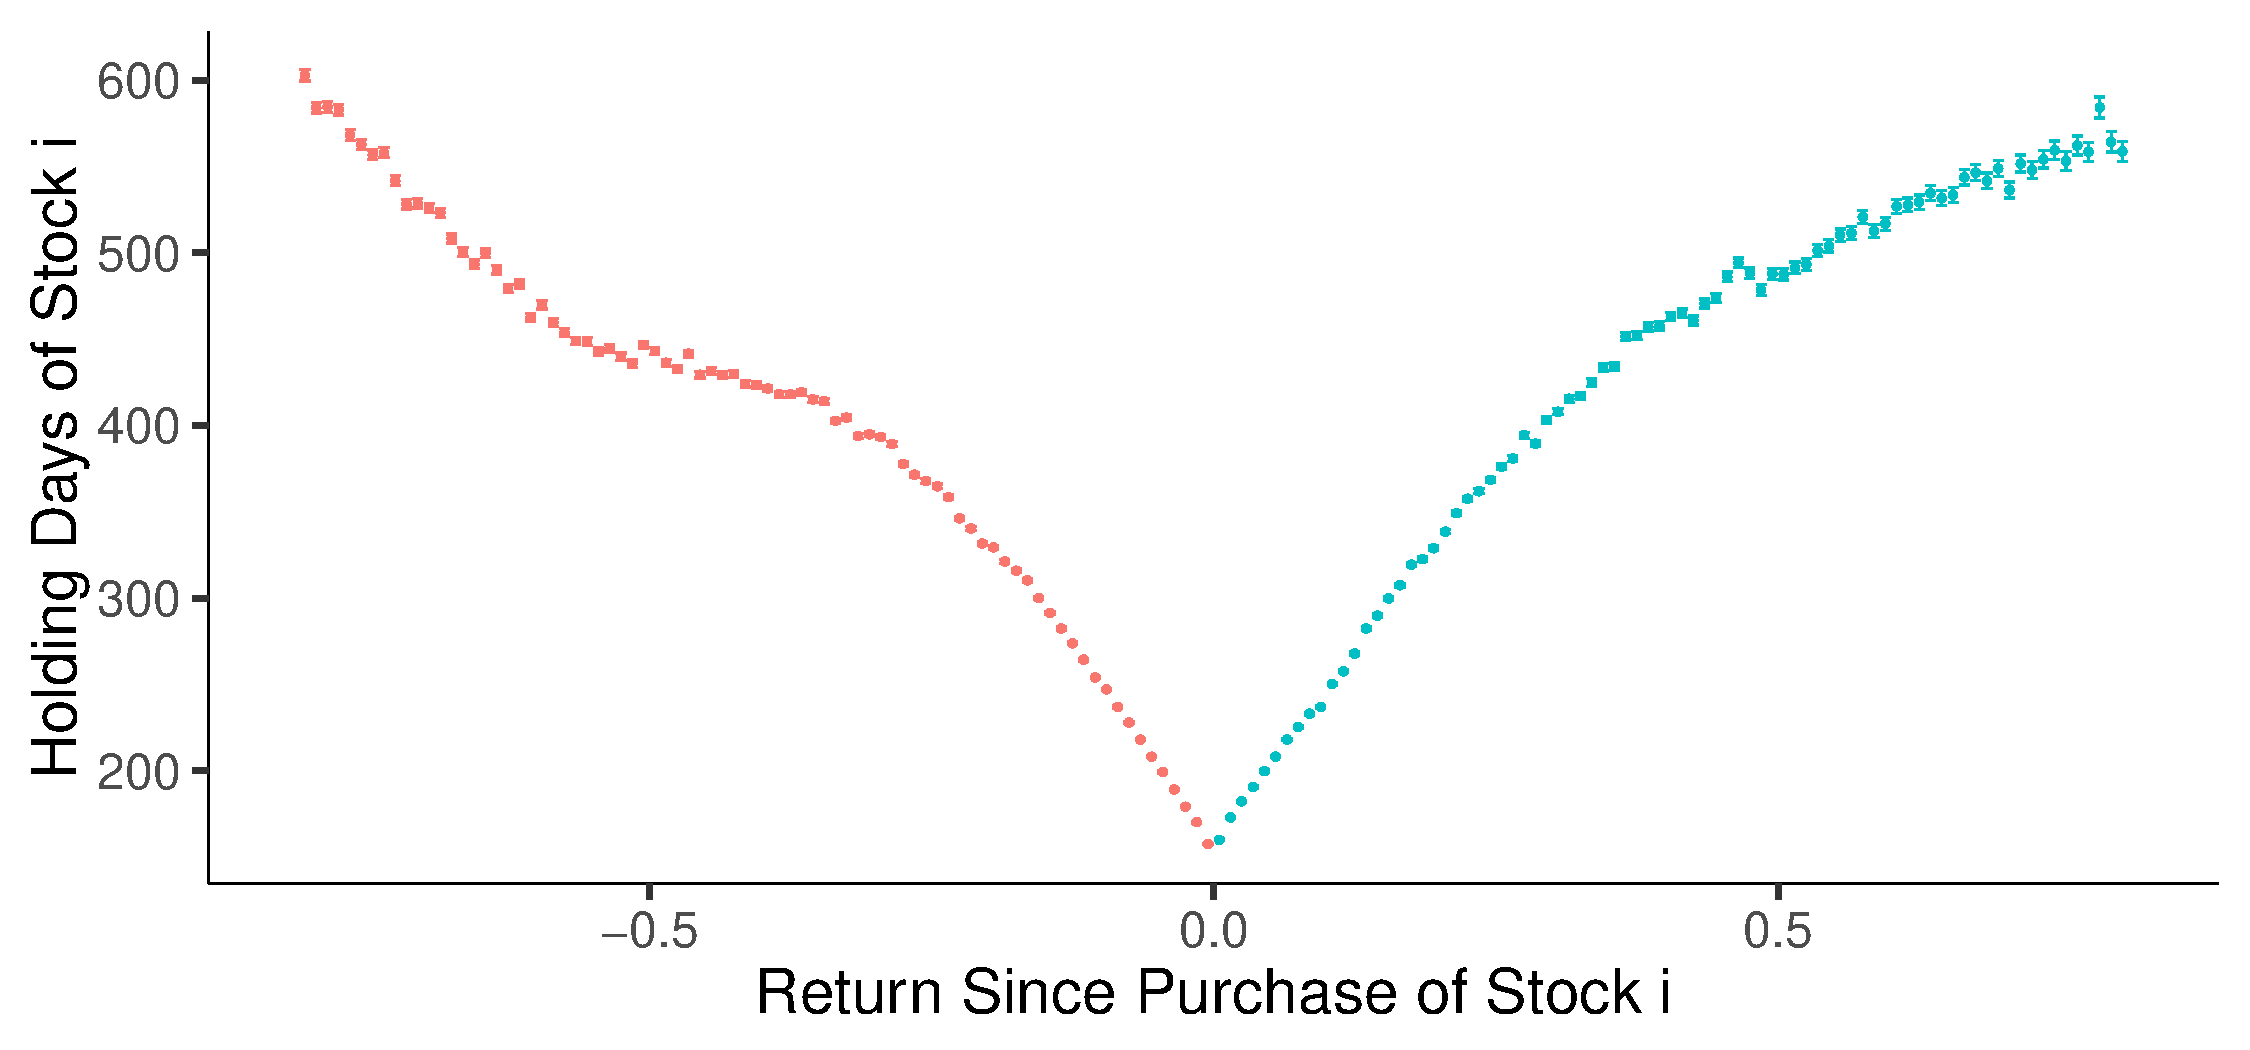
\includegraphics[width=0.8\columnwidth]{barc_holding_days_daily_3.pdf}
	\caption{Holding Days of Stock $i$ (Daily portfolio sample). The bin-width is 0.01. The error bars are 95\% confidence intervals.}
	\label{figure:holding_days}
\end{figure}


\section{Return Distribution}
\label{section:ret}
The distribution of returns since purchase shown in Figure \ref{figure:dist_ret_by_days_less50} already reflects the selling schedule. To illustrate it, we simulate stock prices for 10,000 stocks for 5 years following the geometric Brownian motion (Annualized $\mu=0$ and $\sigma=0.4$). The left panel of Figure \ref{figure:ret} shows the distribution of daily stock returns of those 10,000 stocks for 5 years. By the nature of the Brownian motion, the daily returns are normally distributed. The middle panel shows the distribution of returns since purchase assuming that 10,000 investors bought one of the 10,000 stocks and never sold it. The right panel shows the distribution of returns since purchase assuming that 1\% of investors sold (liquidated) a stock each day. 

The shape of the distribution (i.e., the extent of the concentration around zero return and the convexity of each of the gain and the loss domain) highly depends on the selling probability.



\begin{figure}[H]
	\centering
	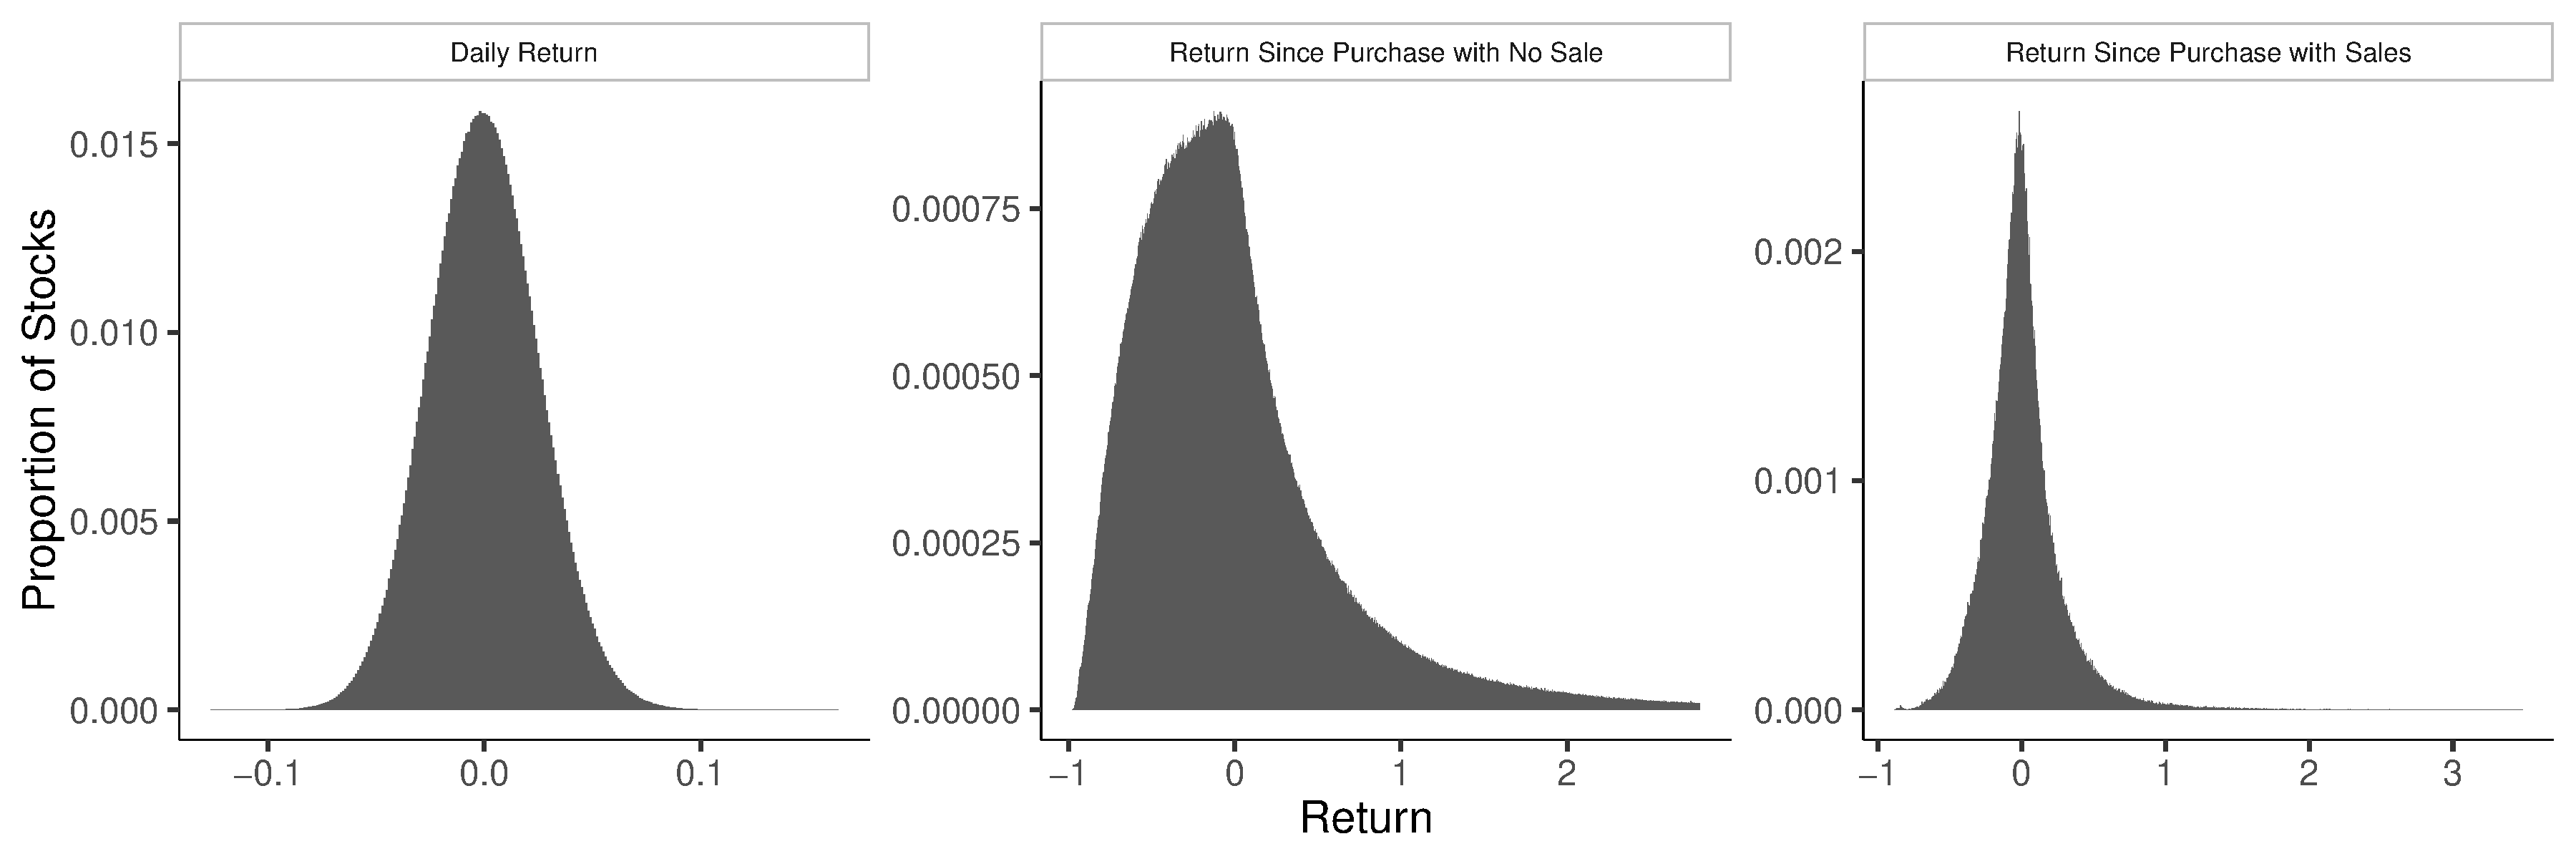
\includegraphics[width=1\columnwidth]{return_dist.pdf}
	\caption{The left, the meddle, and the right panels show the distribution of daily returns, returns since purchase with no sale, and returns since purchase with sales, respectively. The bin-width is 0.001, The extreme 2.5\% returns were excluded from the middle and the right panels.}
	\label{figure:ret}
\end{figure}

\clearpage
\section{More Details of Conditioning on Sell-Days}
\label{section:more_details}

Further, $P(stock~i~is~in~a~sell\mbox{-}day~portfolio)$ can be broken into three parts:

$P(stock~i~is~in~a~sell\mbox{-}day~portfolio) = A+B+C$.\\

\noindent
($A$) Probability of only stock $i$ is sold on the day: 
\begin{equation}
\label{eq:A}
A = P^{daily}_{i}\prod_{j=1}^{N-1}(1-P^{daily}_{j})
\end{equation}


\noindent
($B$) Probability of at least one of stocks $j$ is sold and stock $i$ is not sold on the day.
\begin{equation}
\label{eq:B}
B = (1-P^{daily}_{i})[1-\prod_{j=1}^{N-1}(1-P^{daily}_{j})]
\end{equation}

\noindent
($C$) Probability of stock $i$ is sold and at least one of stocks $j$ is sold and stock $i$ is not sold on the day.
\begin{equation}
\label{eq:C}
C = P^{daily}_{i}[1-\prod_{j=1}^{N-1}(1-P^{daily}_{j})]
\end{equation}

Also, $B$ can be divided into two parts: $B=B_1B_2$.\\

\noindent
($B_{1}$) Probability of stock $i$ is not sold.
\begin{equation}
\label{eq:B1}
B_1 = 1-P^{daily}_{i}
\end{equation}

\noindent
($B_{2}$) Probability of at least one of stocks $j$ is sold.
\begin{equation}
\label{eq:B2}
B_2 = 1-\prod_{j=1}^{N-1}(1-P^{daily}_{j})
\end{equation}

\noindent

Because $P^{daily}_{i} = A+C$, all the above together,

\begin{equation}
\label{eq:PABC}
P^{sell\mbox{-}day}_{i} = \frac{A+C}{A+B+C} = \frac{P^{daily}_{i}}{P^{daily}_{i}+B} = \frac{P^{daily}_{i}}{P^{daily}_{i}+(1-P^{daily}_{i})B_2}
\end{equation}


%\noindent
%\HS{The effect of $N$ on $P(stock~i~in~a~sell\mbox{-}day~portfolio)$ described in the point i above mechanically boosts the composition sensitivity of the disposition effect in the sell-day portfolio sample while a milder composition sensitivity is still observed in the daily portfolio sample. I will revise our two-stage model paper mainly using daily portfolio sample.}  
%\clearpage

\begin{figure}[H]
	\centering
	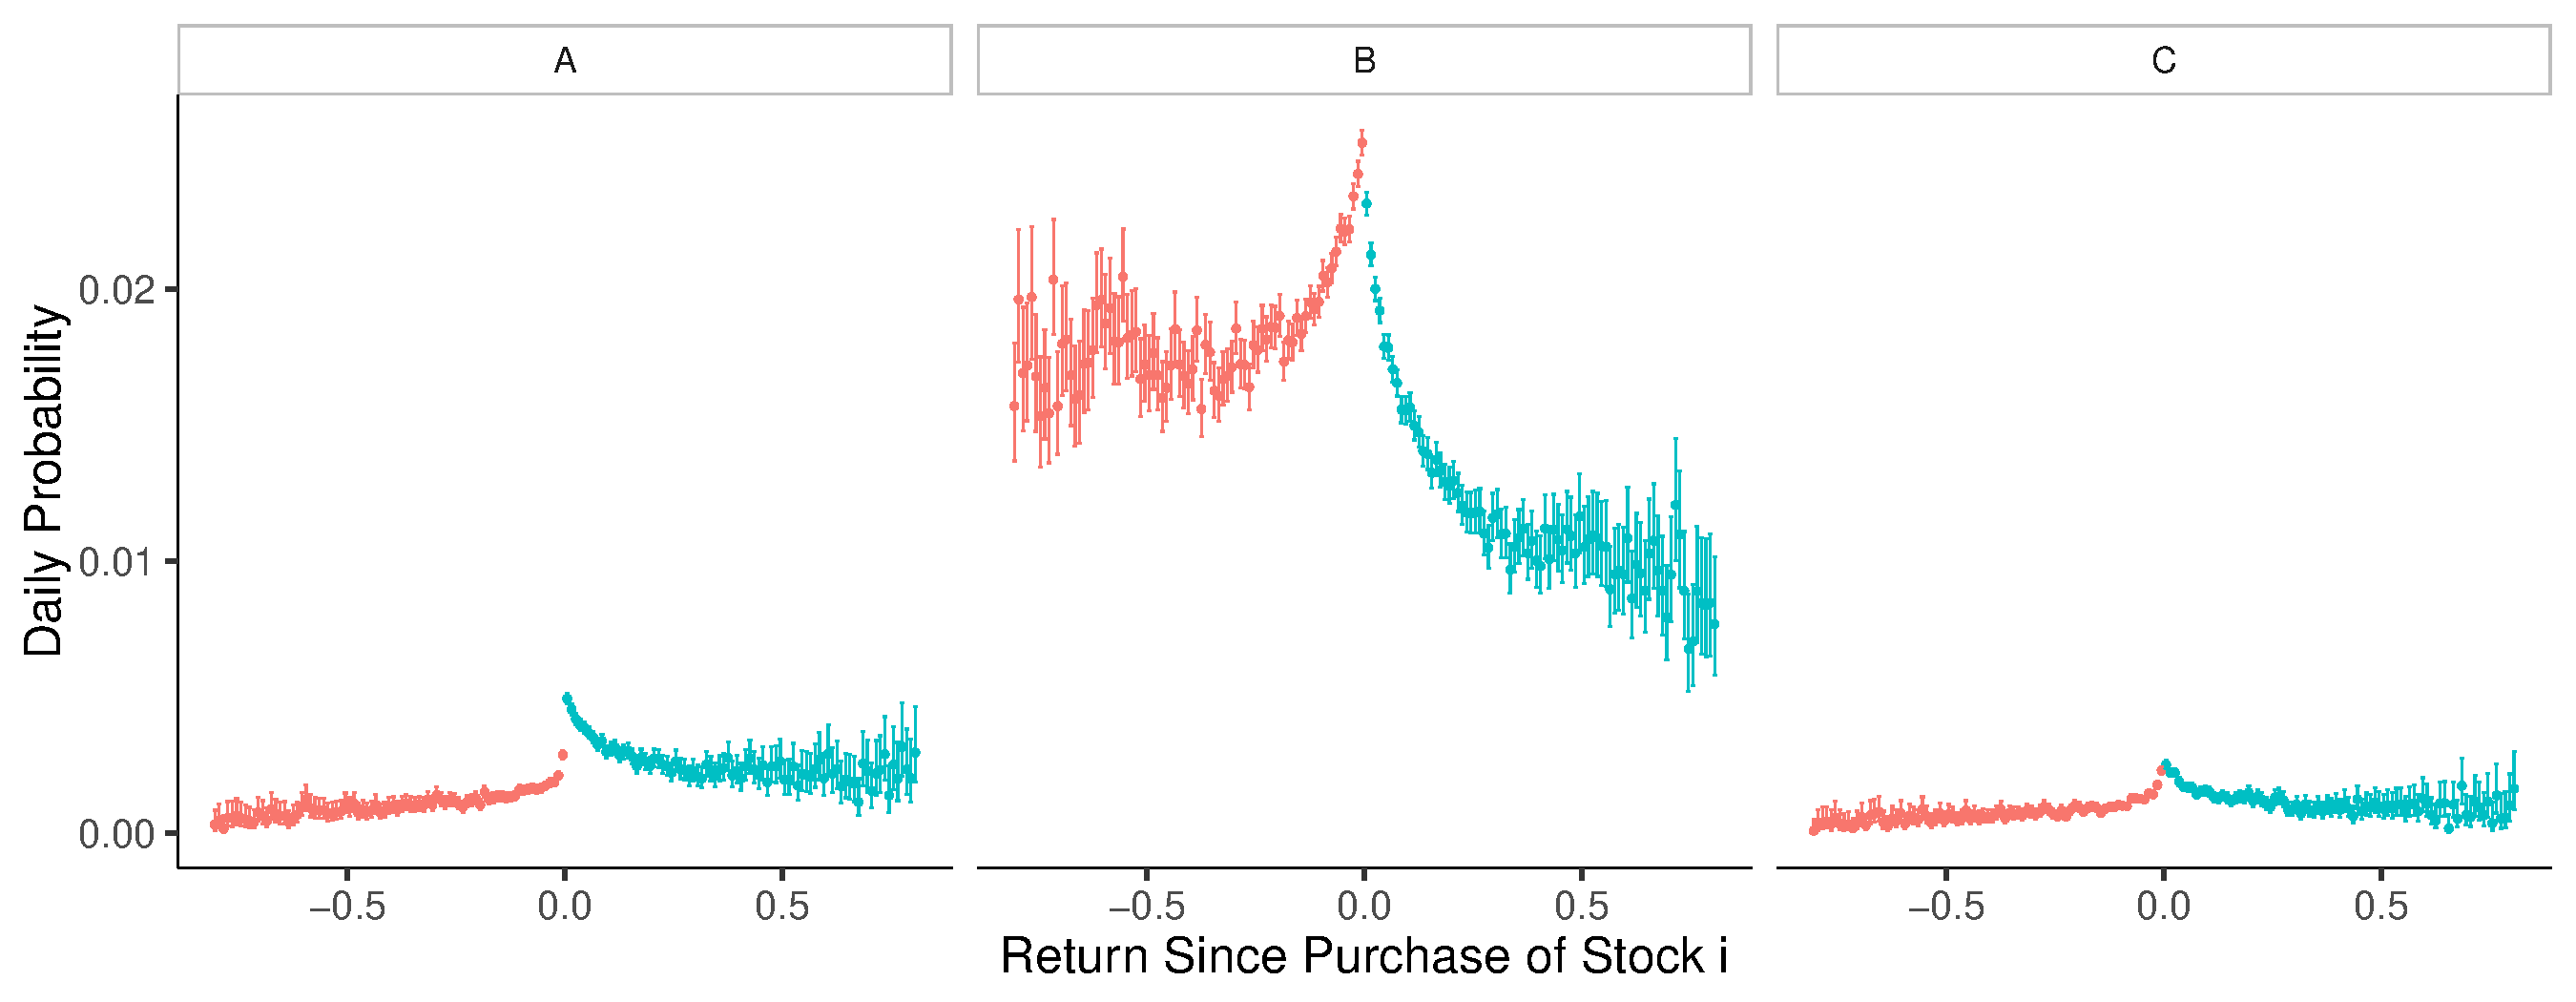
\includegraphics[width=1\columnwidth]{barc_ABC_NG1_NL1_3.pdf}
	\caption{\small A, B, and C (Daily portfolio sample given $NG\geq1$ and $NL\geq1$). The bin-width is 0.01. The error bars are 95\% confidence intervals.}
	\label{figure:prop_ABC_NG1NL1}
\end{figure}

\begin{figure}[H]
	\centering
	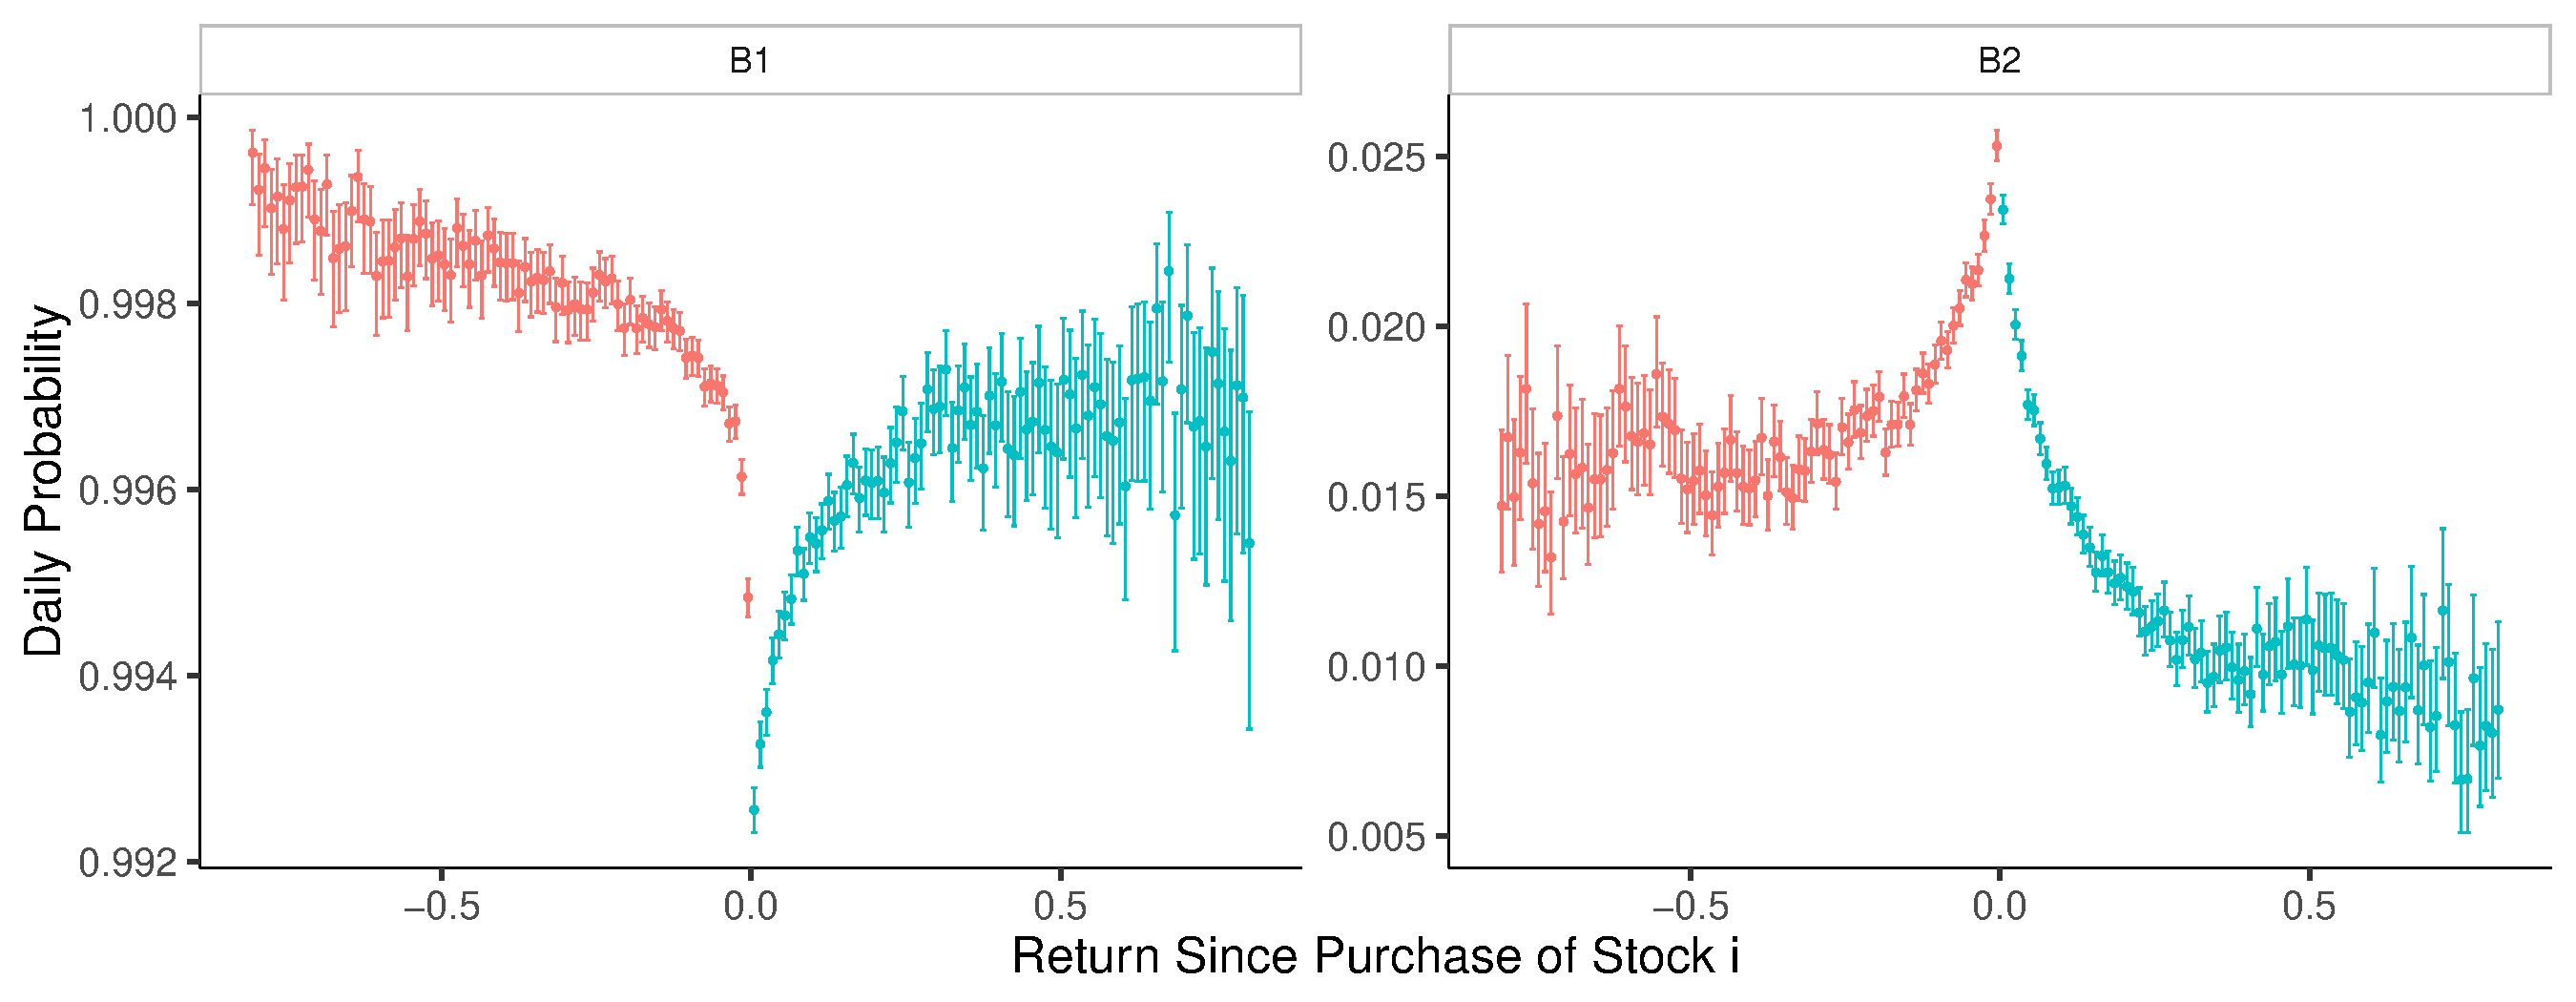
\includegraphics[width=1\columnwidth]{barc_B12_NG1_NL1_3.pdf}
	\caption{\small B1 and B2 (Daily portfolio sample given $NG\geq1$ and $NL\geq1$). The bin-width is 0.01. The error bars are 95\% confidence intervals. $B_{1}=1-P^{daily}_{i}$.}
	\label{figure:prop_B12_NG1NL1}
\end{figure}

\end{appendices}

\pagebreak
\bibliographystyle{plainnat}
\bibliography{local_refs2new}

\end{document}

\section{Unused Figures}
\begin{figure}[H]
	\centering
	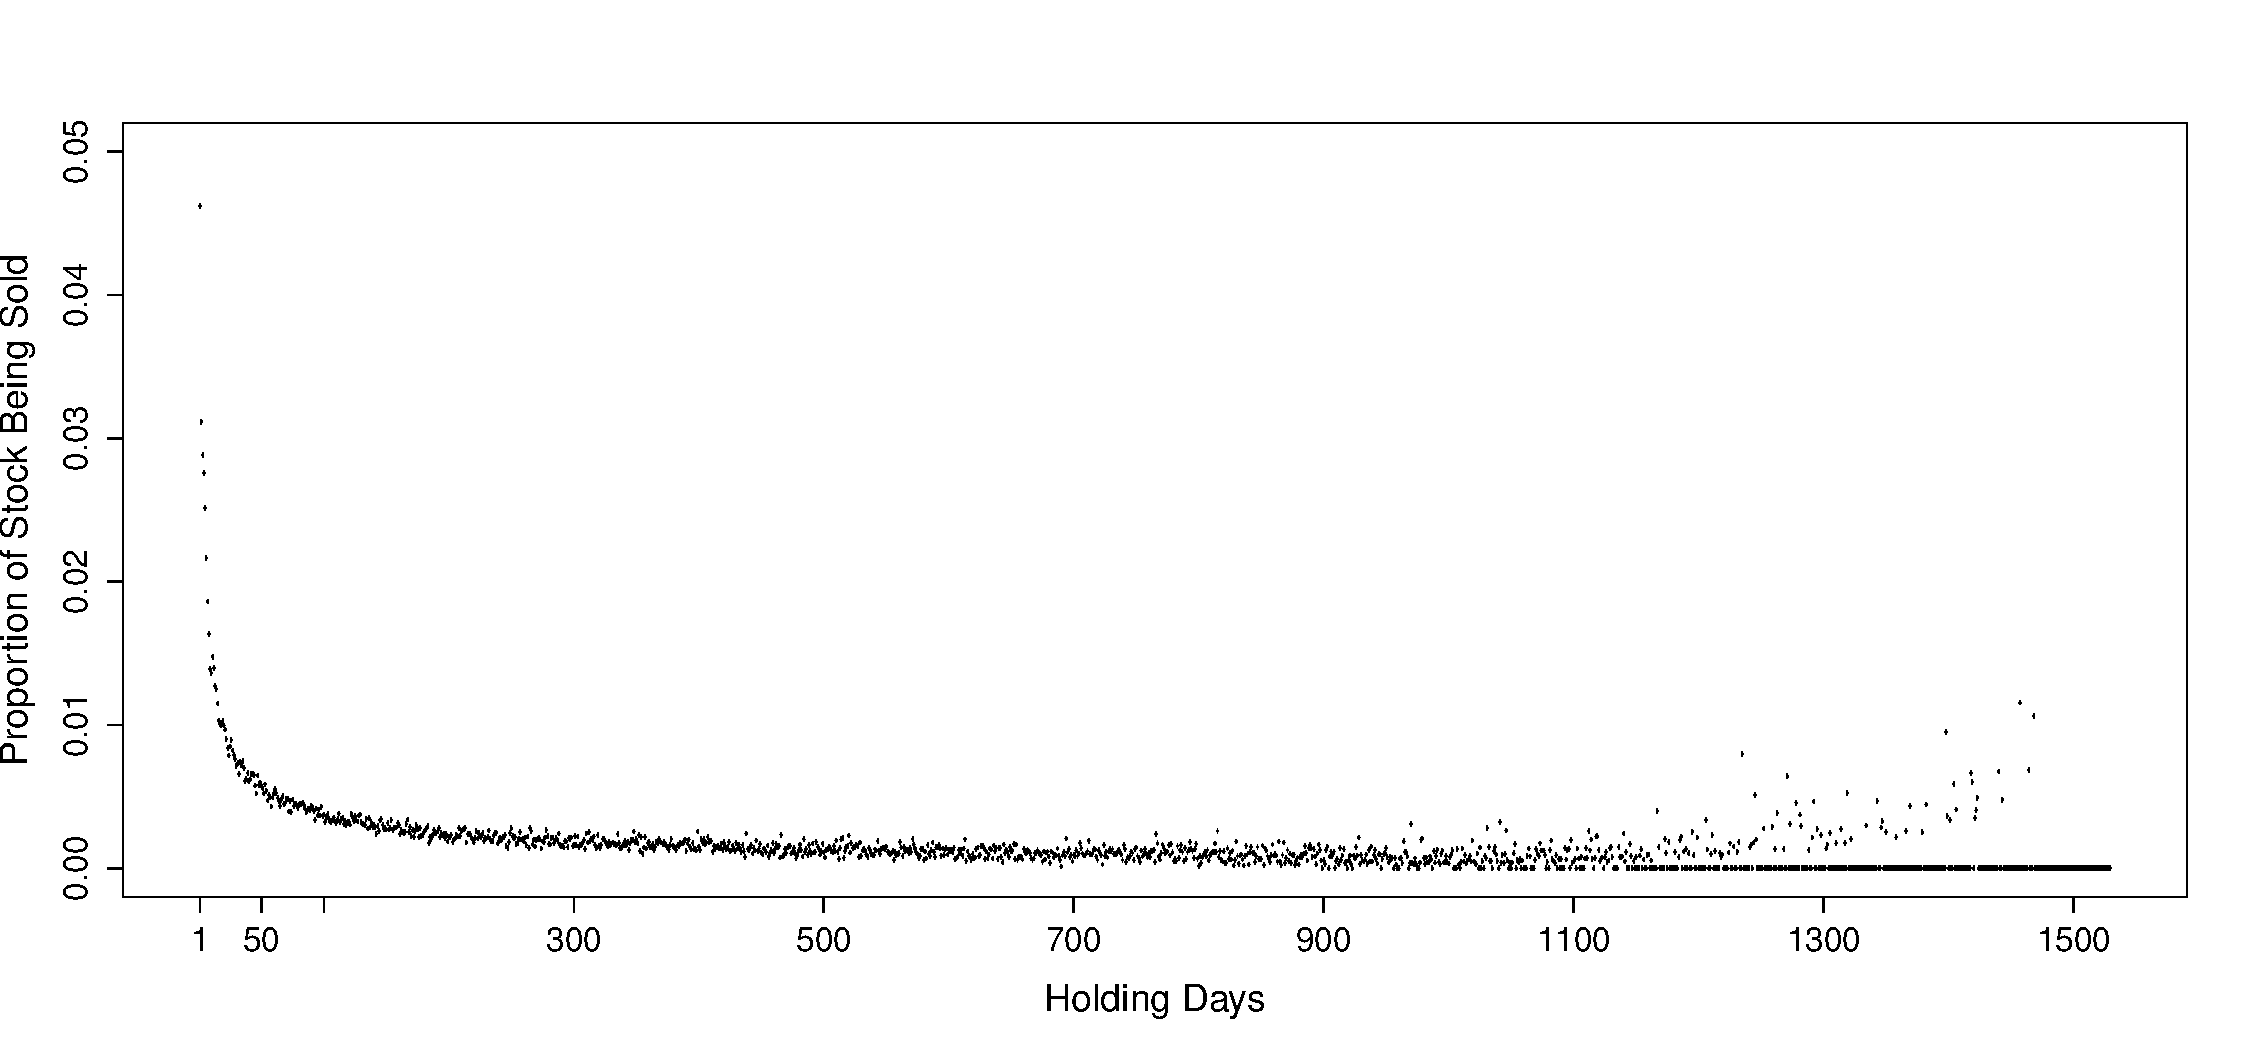
\includegraphics[width=0.8\columnwidth]{barc_prop_holding_days.pdf}
	\caption{Proportion of stocks being sold ($P^{daily}_{i}$; Daily portfolio sample) as a function of holding days.}
	\label{figure:prop_on_days}
\end{figure}

\begin{figure}[H]
	\centering
	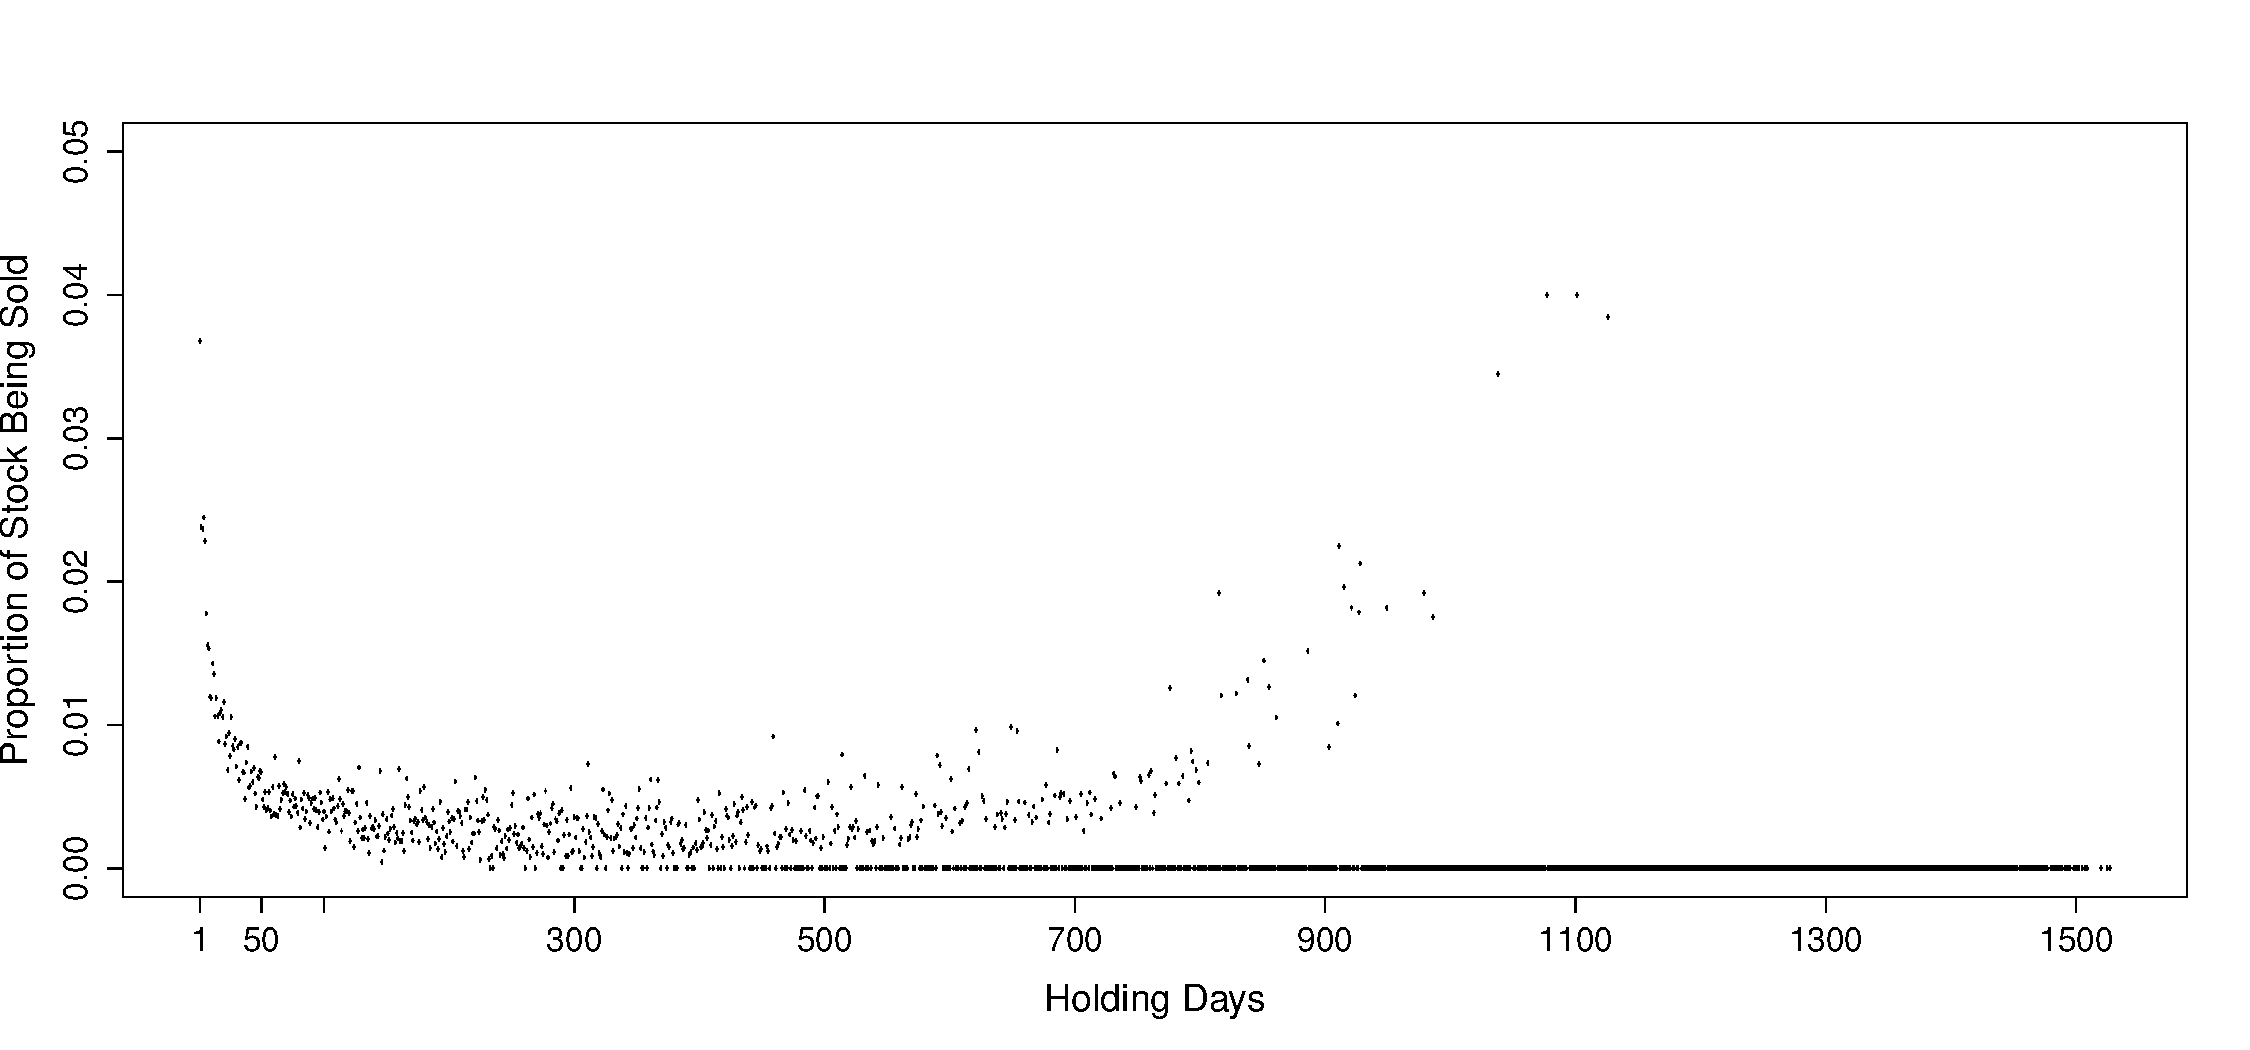
\includegraphics[width=0.8\columnwidth]{barc_prop_holding_days_around_zero.pdf}
	\caption{Proportion of stocks being sold ($P^{daily}_{i}$; Daily portfolio sample) as a function of holding days for stocks whose return is between -0.01 and 0.01.}
	\label{figure:prop_on_days_around_zero}
\end{figure}

%\begin{figure}[H]
%	\centering
%	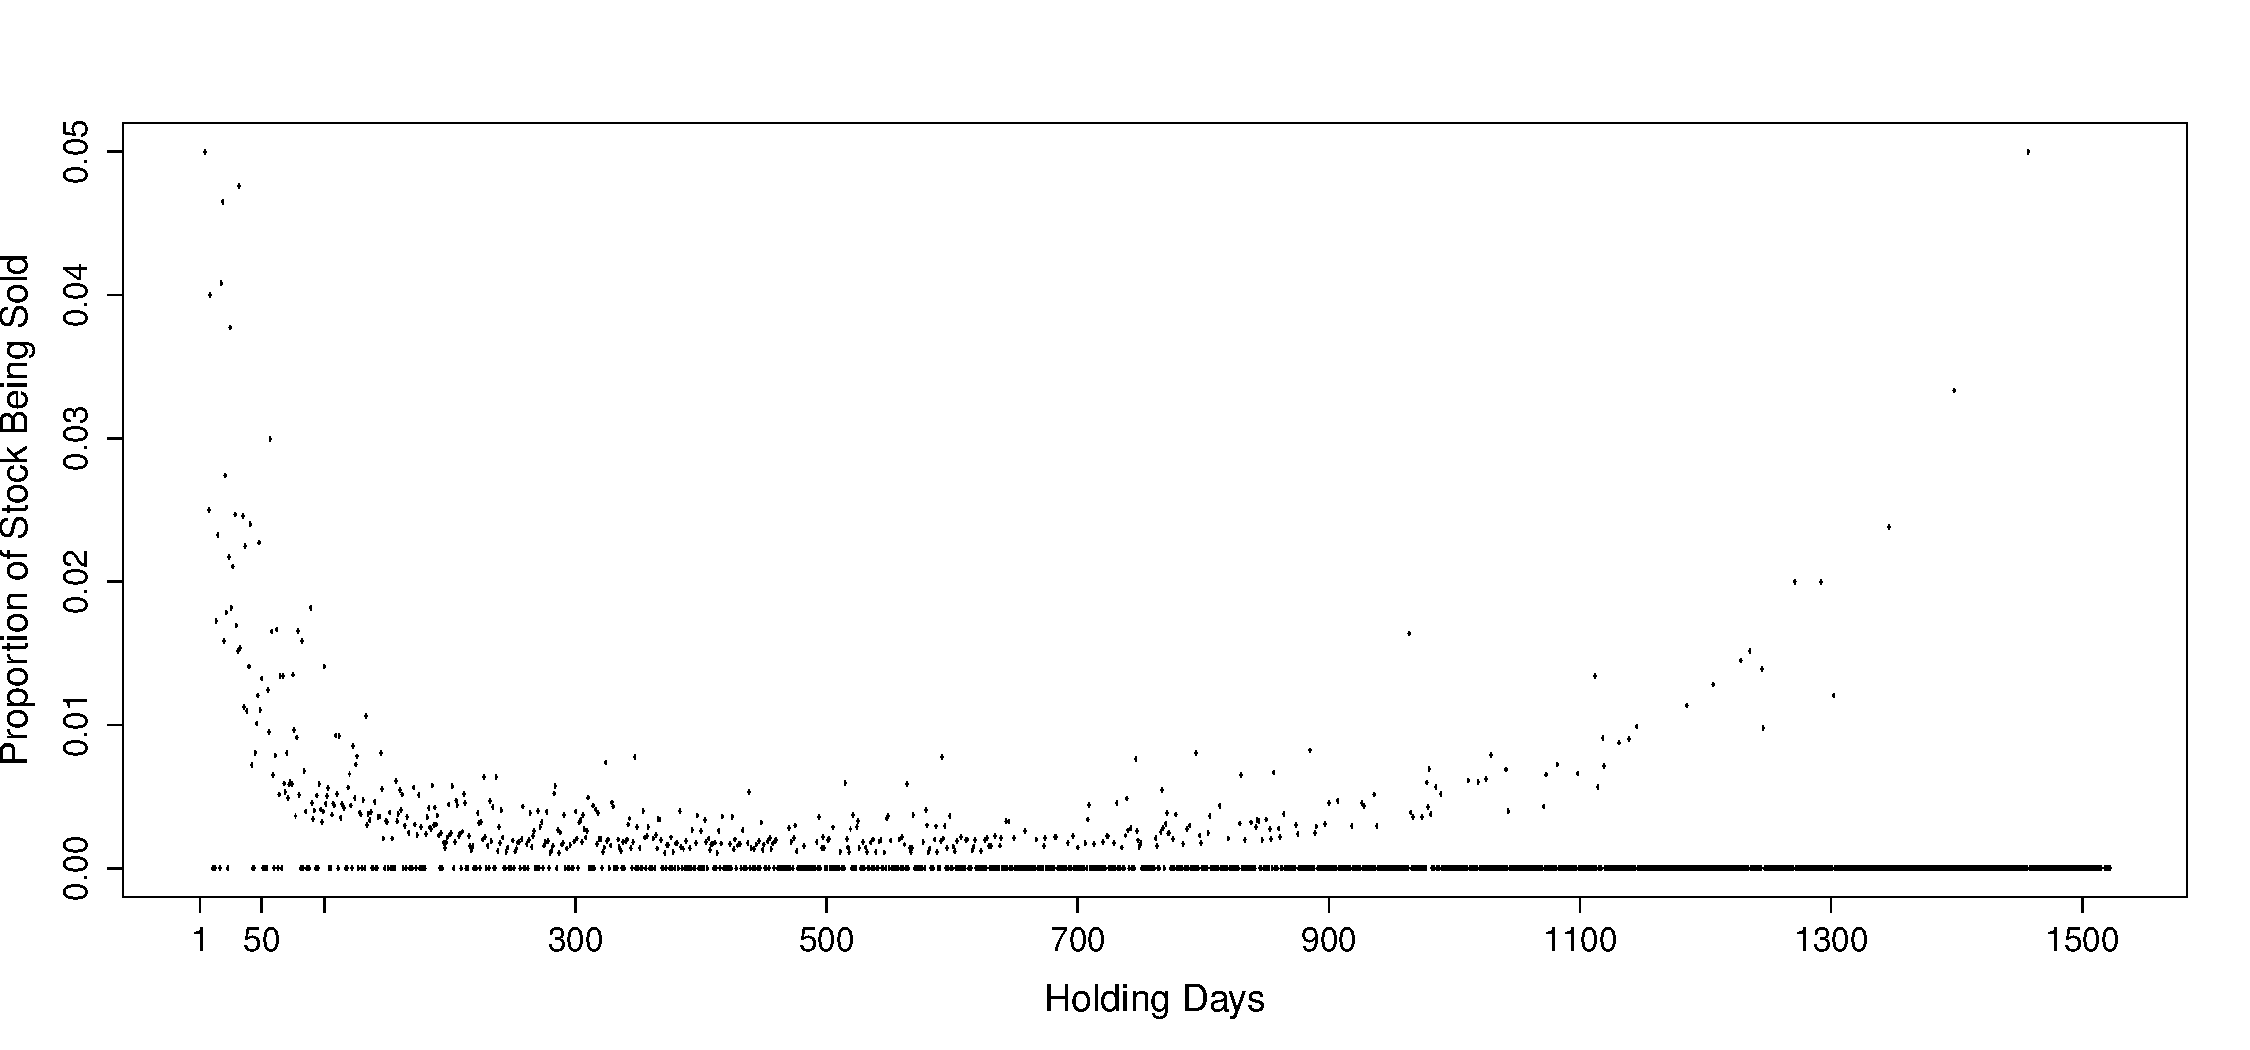
\includegraphics[width=0.8\columnwidth]{barc_prop_holding_days_large_abs_ret.pdf}
%	\caption{Proportion of stocks being sold ($P^{daily}_{i}$; Daily portfolio sample) as a function of holding days.}
%	\label{figure:prop_on_days_large_abs}
%\end{figure}



\begin{figure}[H]
	\centering
	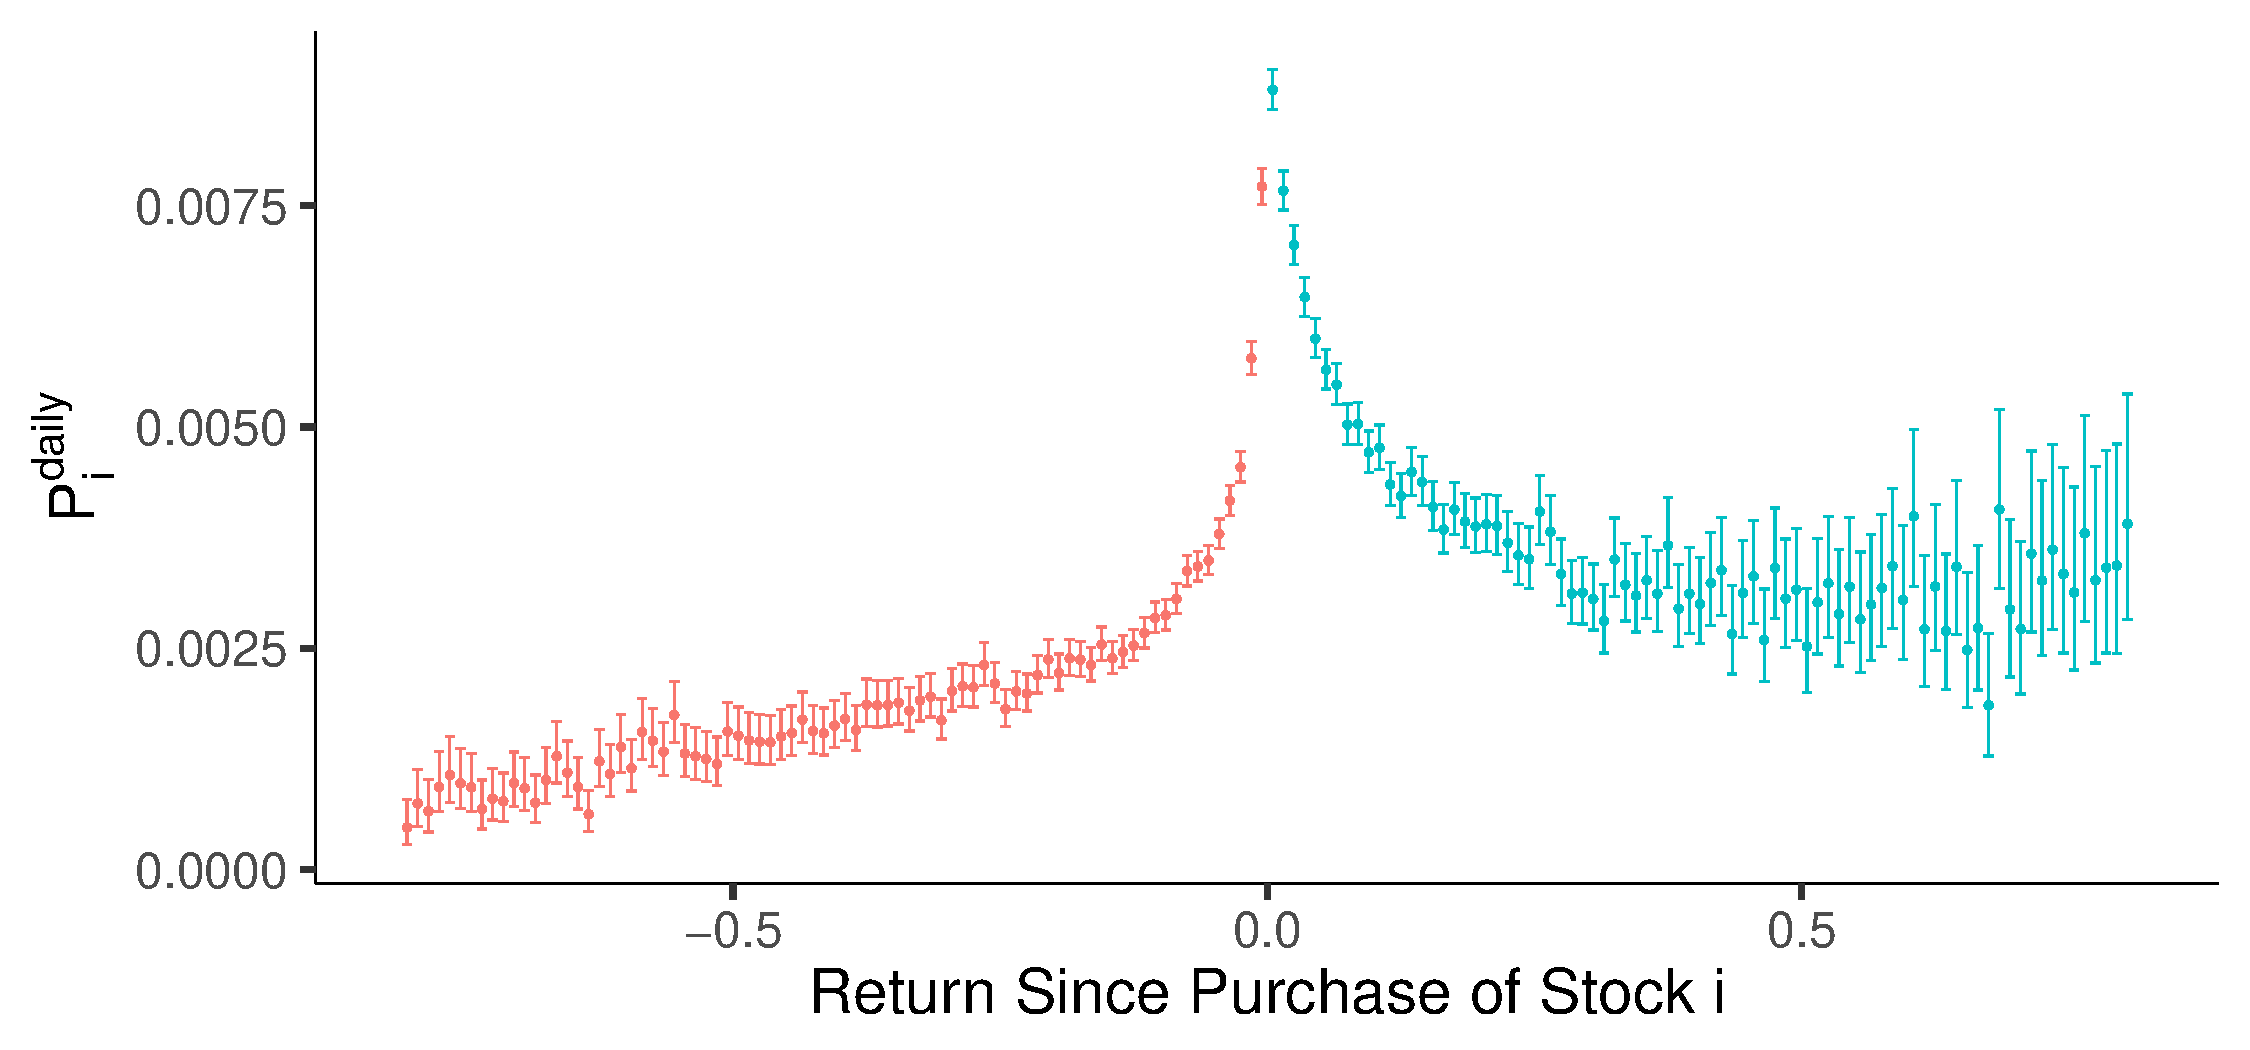
\includegraphics[width=0.8\columnwidth]{barc_schedule_daily_all_3.pdf}
	\caption{Proportion of stocks being sold ($P^{daily}_{i}$; Daily portfolio sample). The bin-width is 0.01. The error bars are 95\% confidence intervals.}
	\label{figure:prop_all}
\end{figure}


\begin{figure}[H]
	\centering
	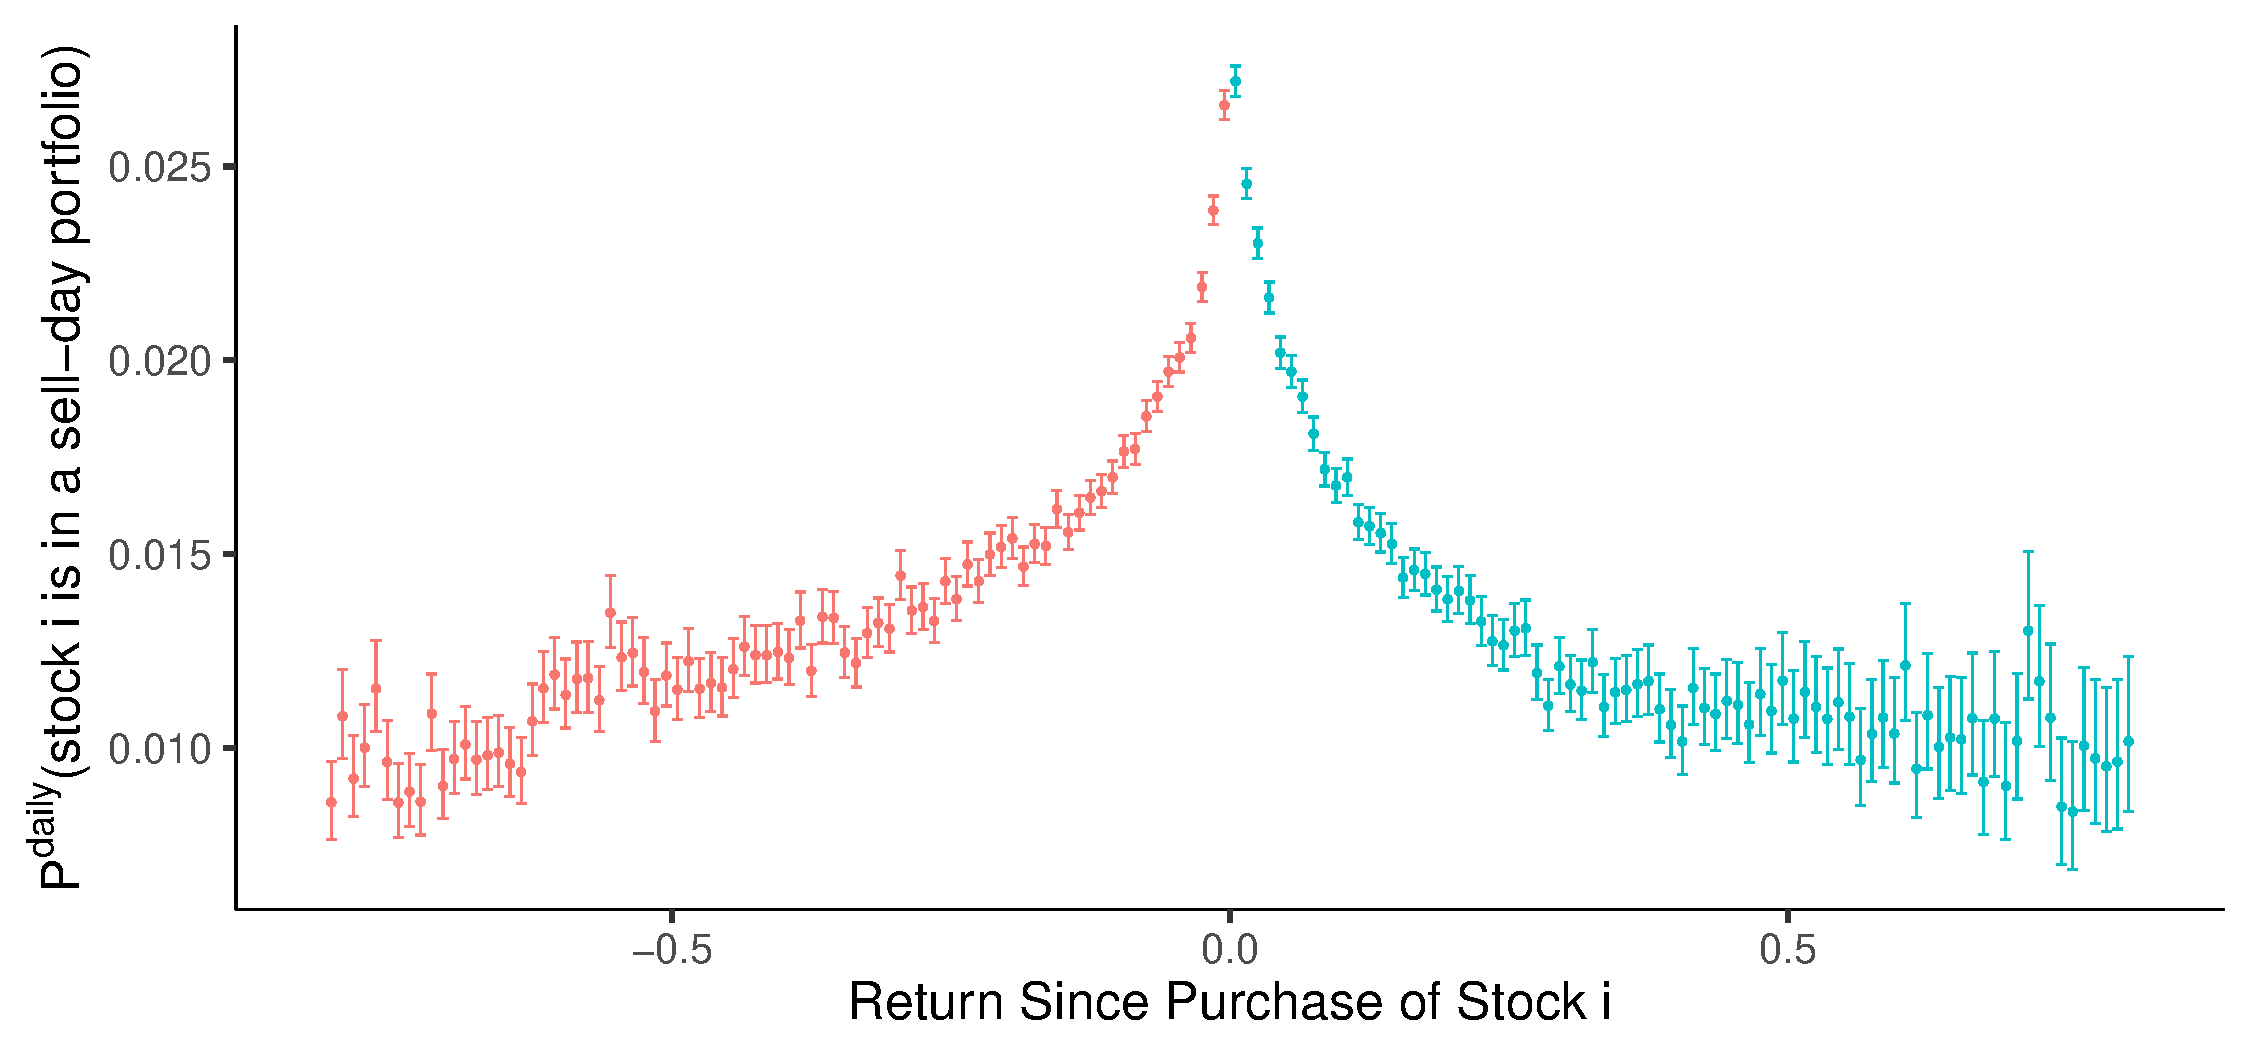
\includegraphics[width=0.8\columnwidth]{barc_port_sell_3.pdf}
	\caption{\small Proportion of stocks being included in a sell-day portfolio (Daily portfolio sample). The bin-width is 0.01. The error bars are 95\% confidence intervals.}
	\label{figure:prop_sell_day}
\end{figure}



\begin{figure}[H]
	\centering
	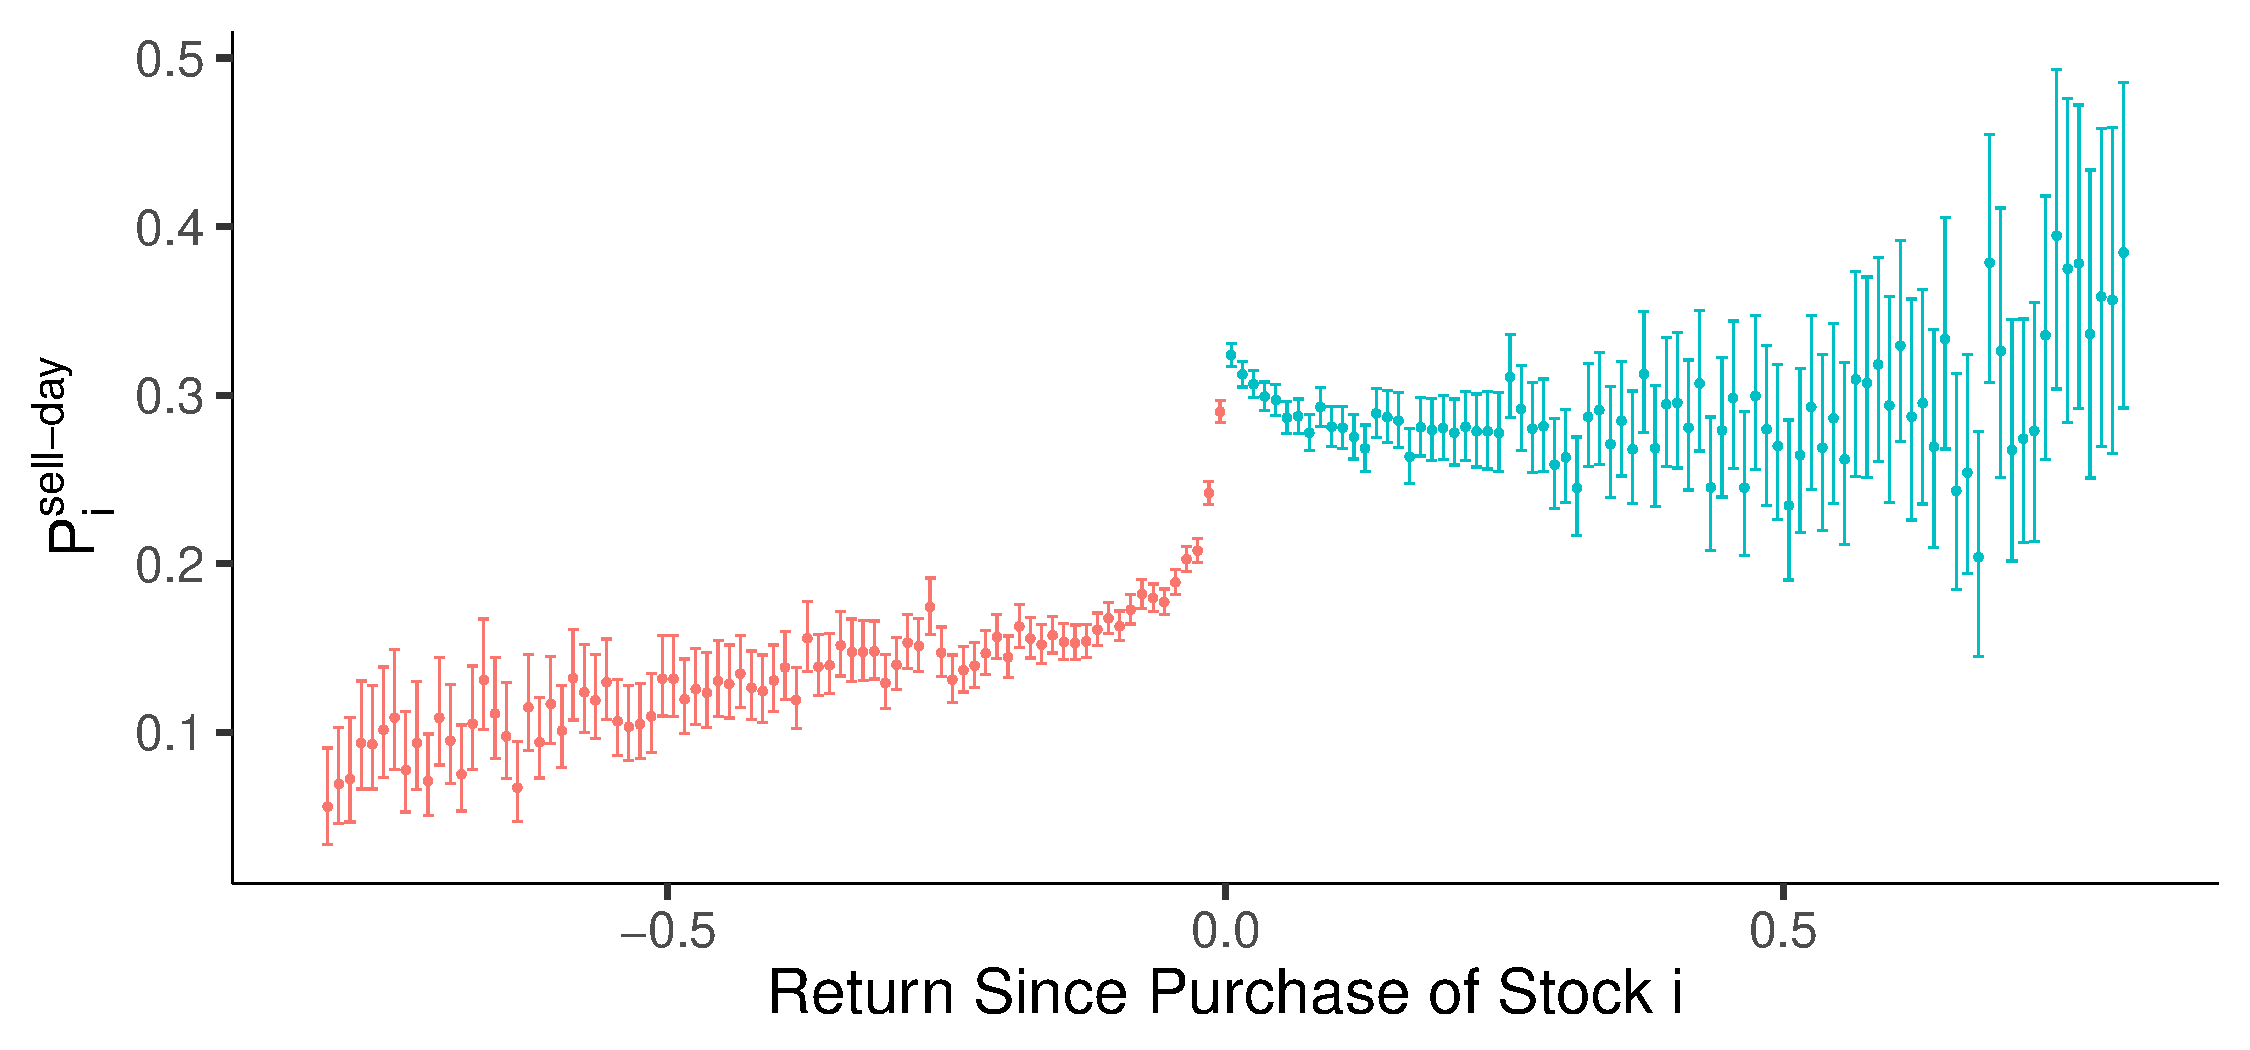
\includegraphics[width=0.8\columnwidth]{barc_schedule_sell_day_3.pdf}
	\caption{\small Proportion of stocks being sold ($P^{sell\mbox{-}day}_{i}$; Sell-day portfolio sample). The bin-width is 0.01. The error bars are 95\% confidence intervals.}
	\label{figure:prop_sell_days}
\end{figure}

\begin{figure}[H]
	\centering
	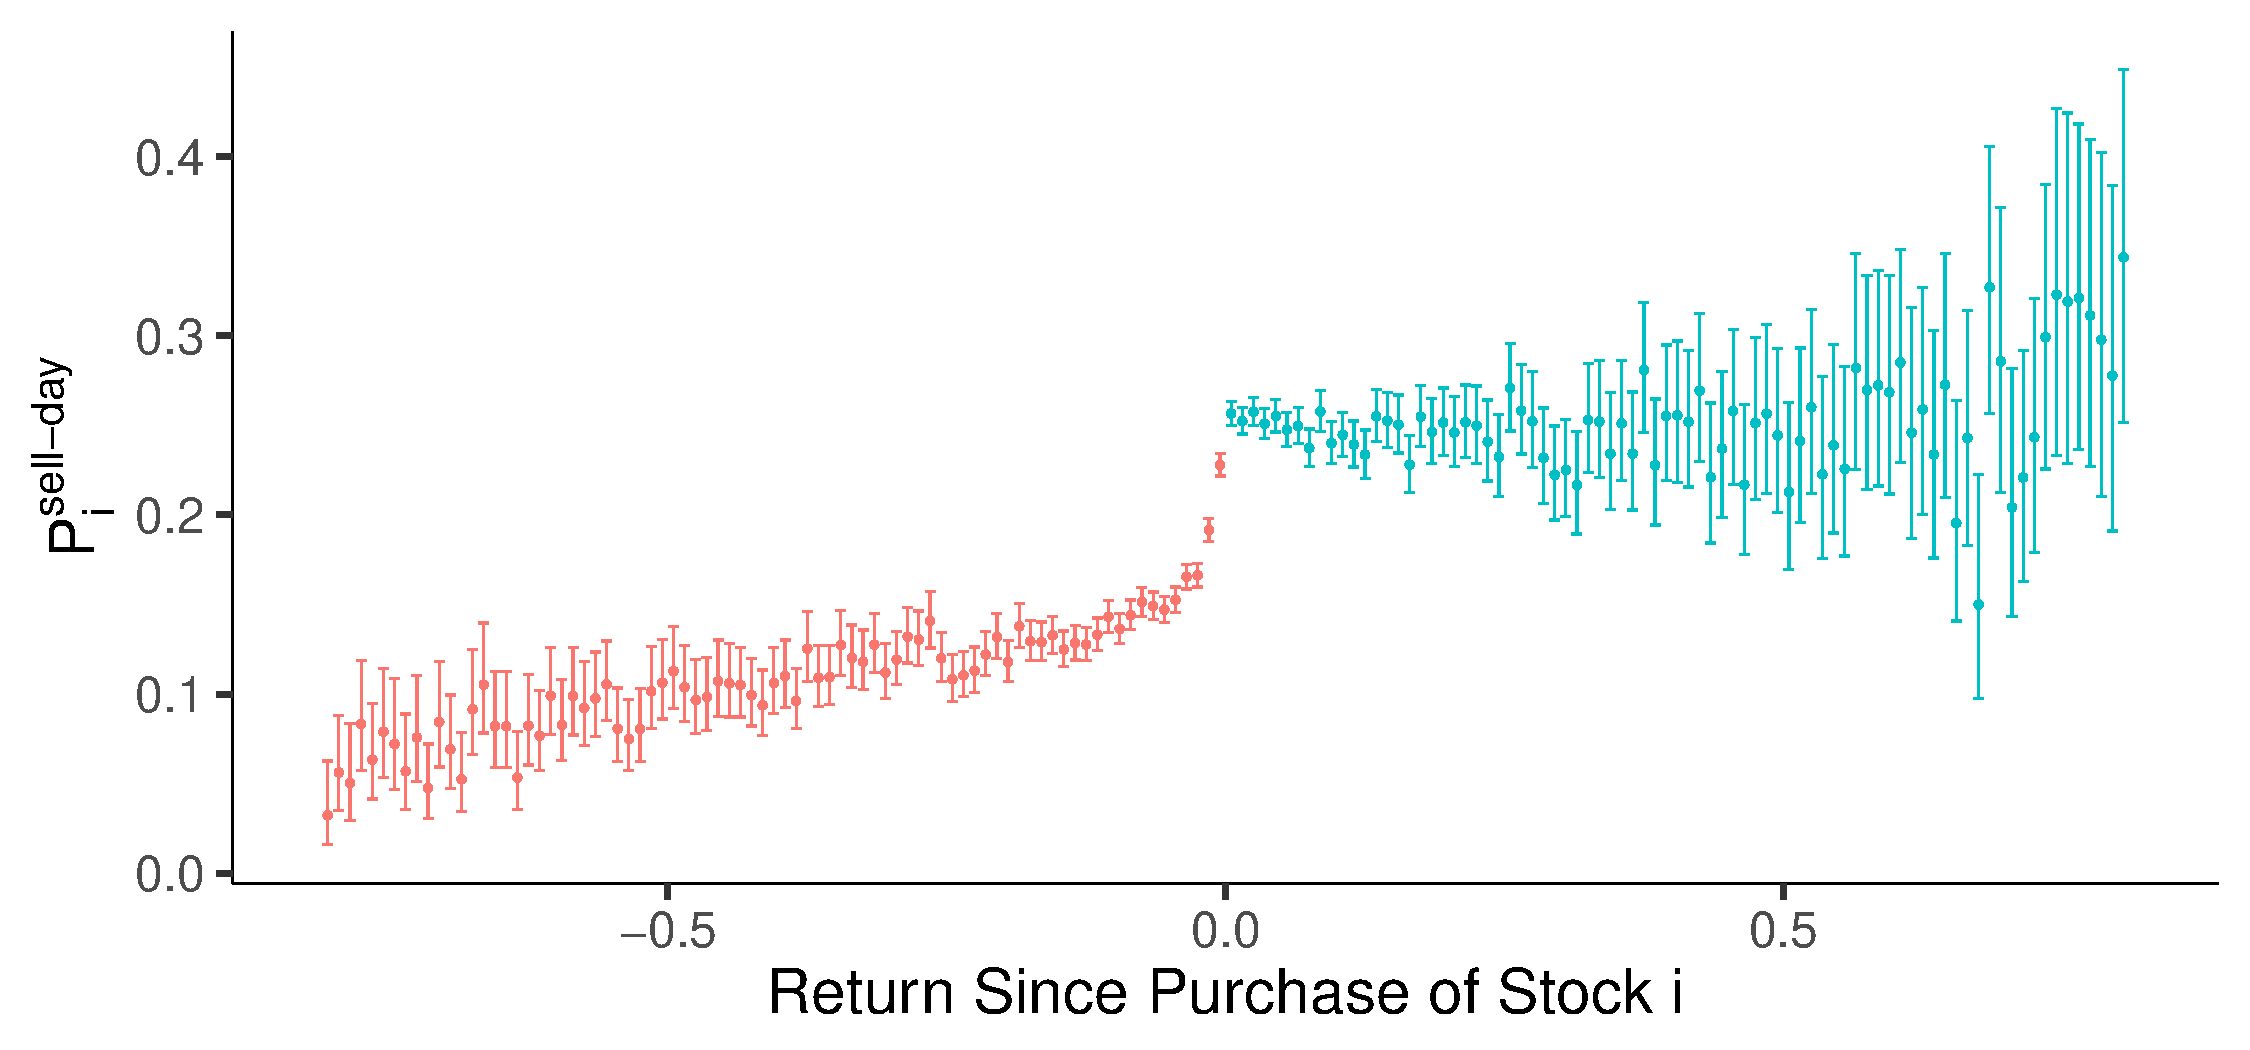
\includegraphics[width=0.8\columnwidth]{barc_schedule_sell_day_N2_3.pdf}
	\caption{\small Proportion of stocks being sold ($P^{sell\mbox{-}day}_{i}$; Sell-day portfolio sample given $N\geq2$). The bin-width is 0.01. The error bars are 95\% confidence intervals.}
	\label{figure:prop_sell_days_n2}
\end{figure}


\begin{figure}[H]
	\centering
	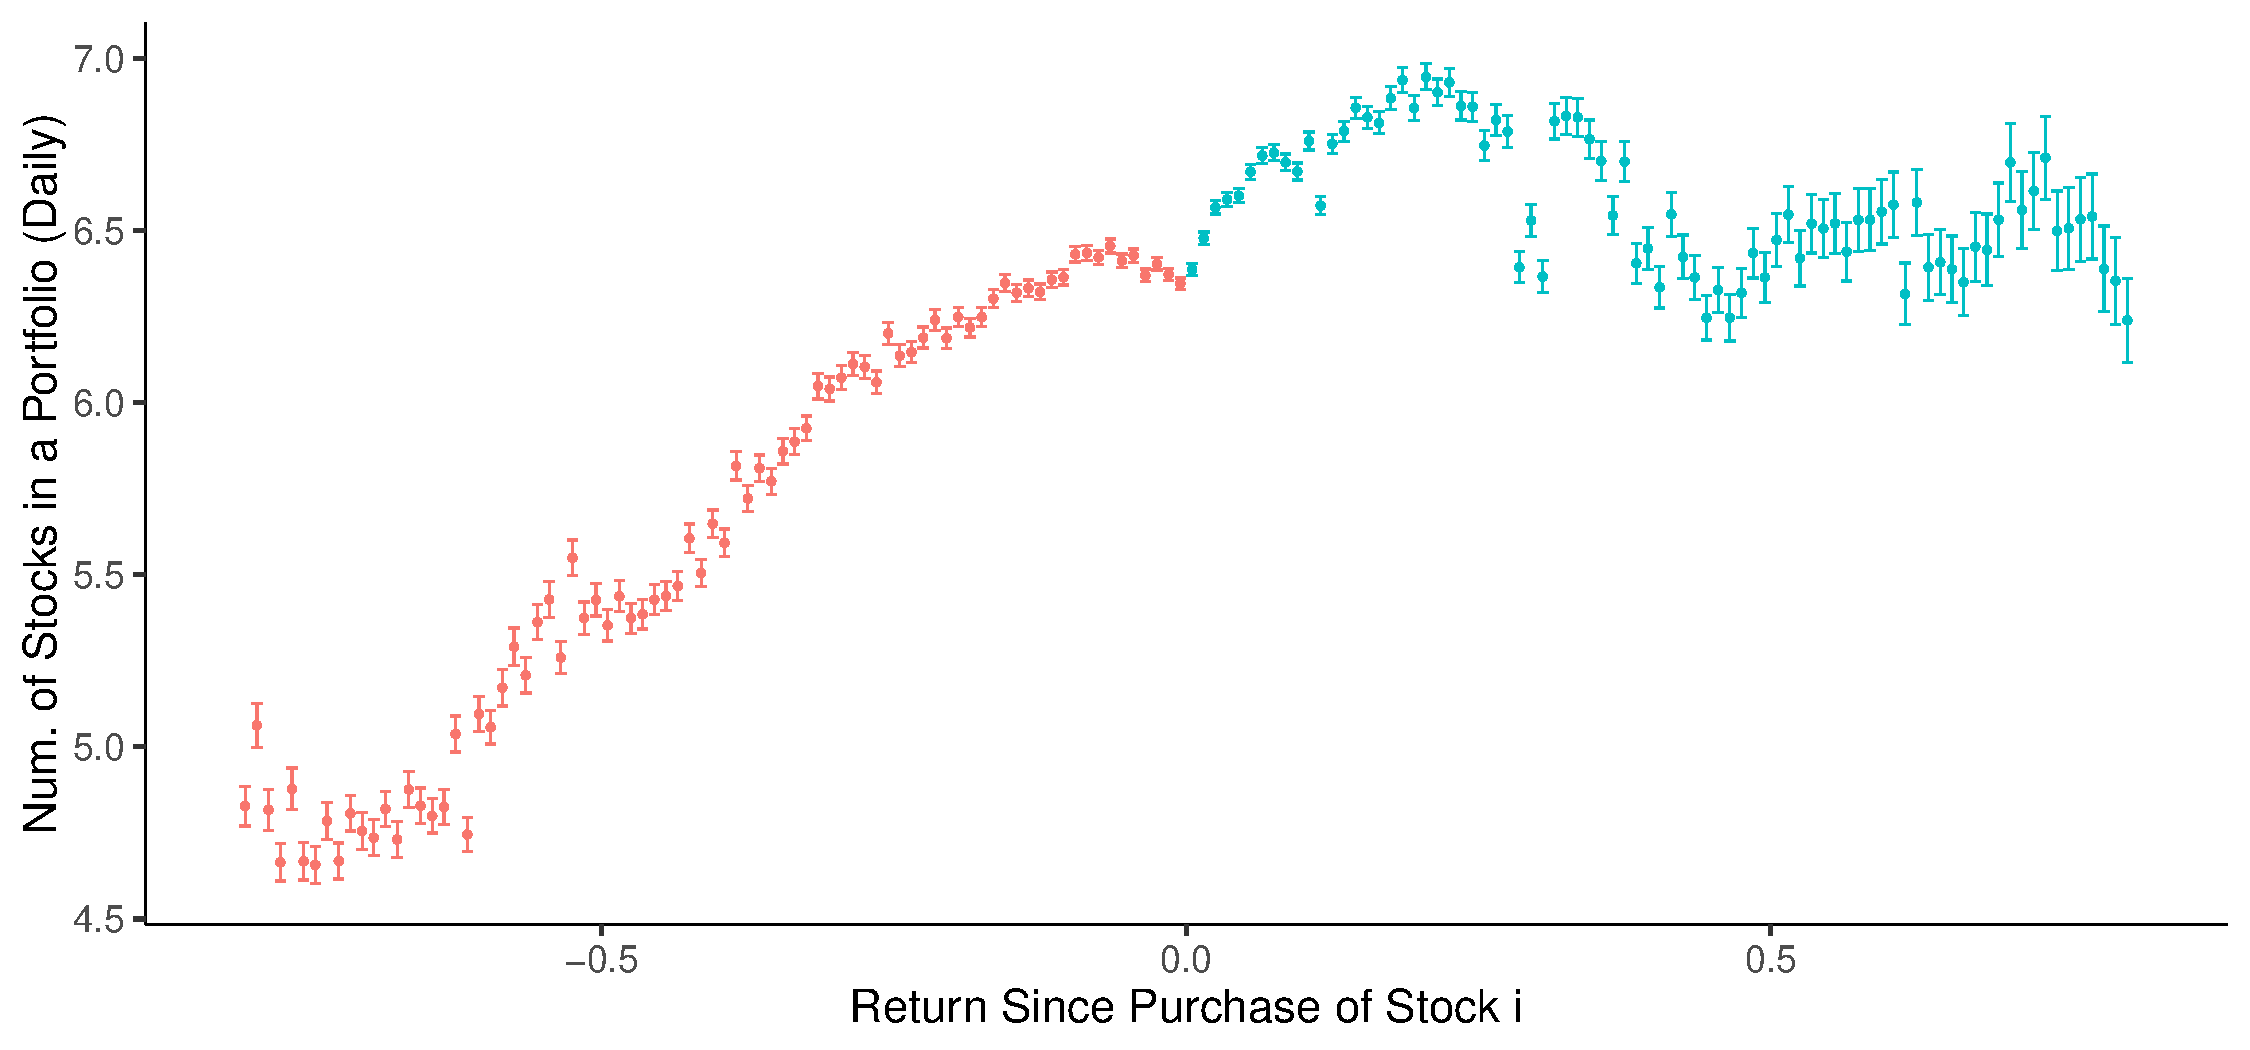
\includegraphics[width=0.8\columnwidth]{barc_num_stocks_daily_3.pdf}
	\caption{\small Number of stocks in a portfolio on return since purchase (Daily portfolio sample)}
	\label{figure:N_on_return}
\end{figure}

\pagebreak

\begin{figure}[H]
	\centering
	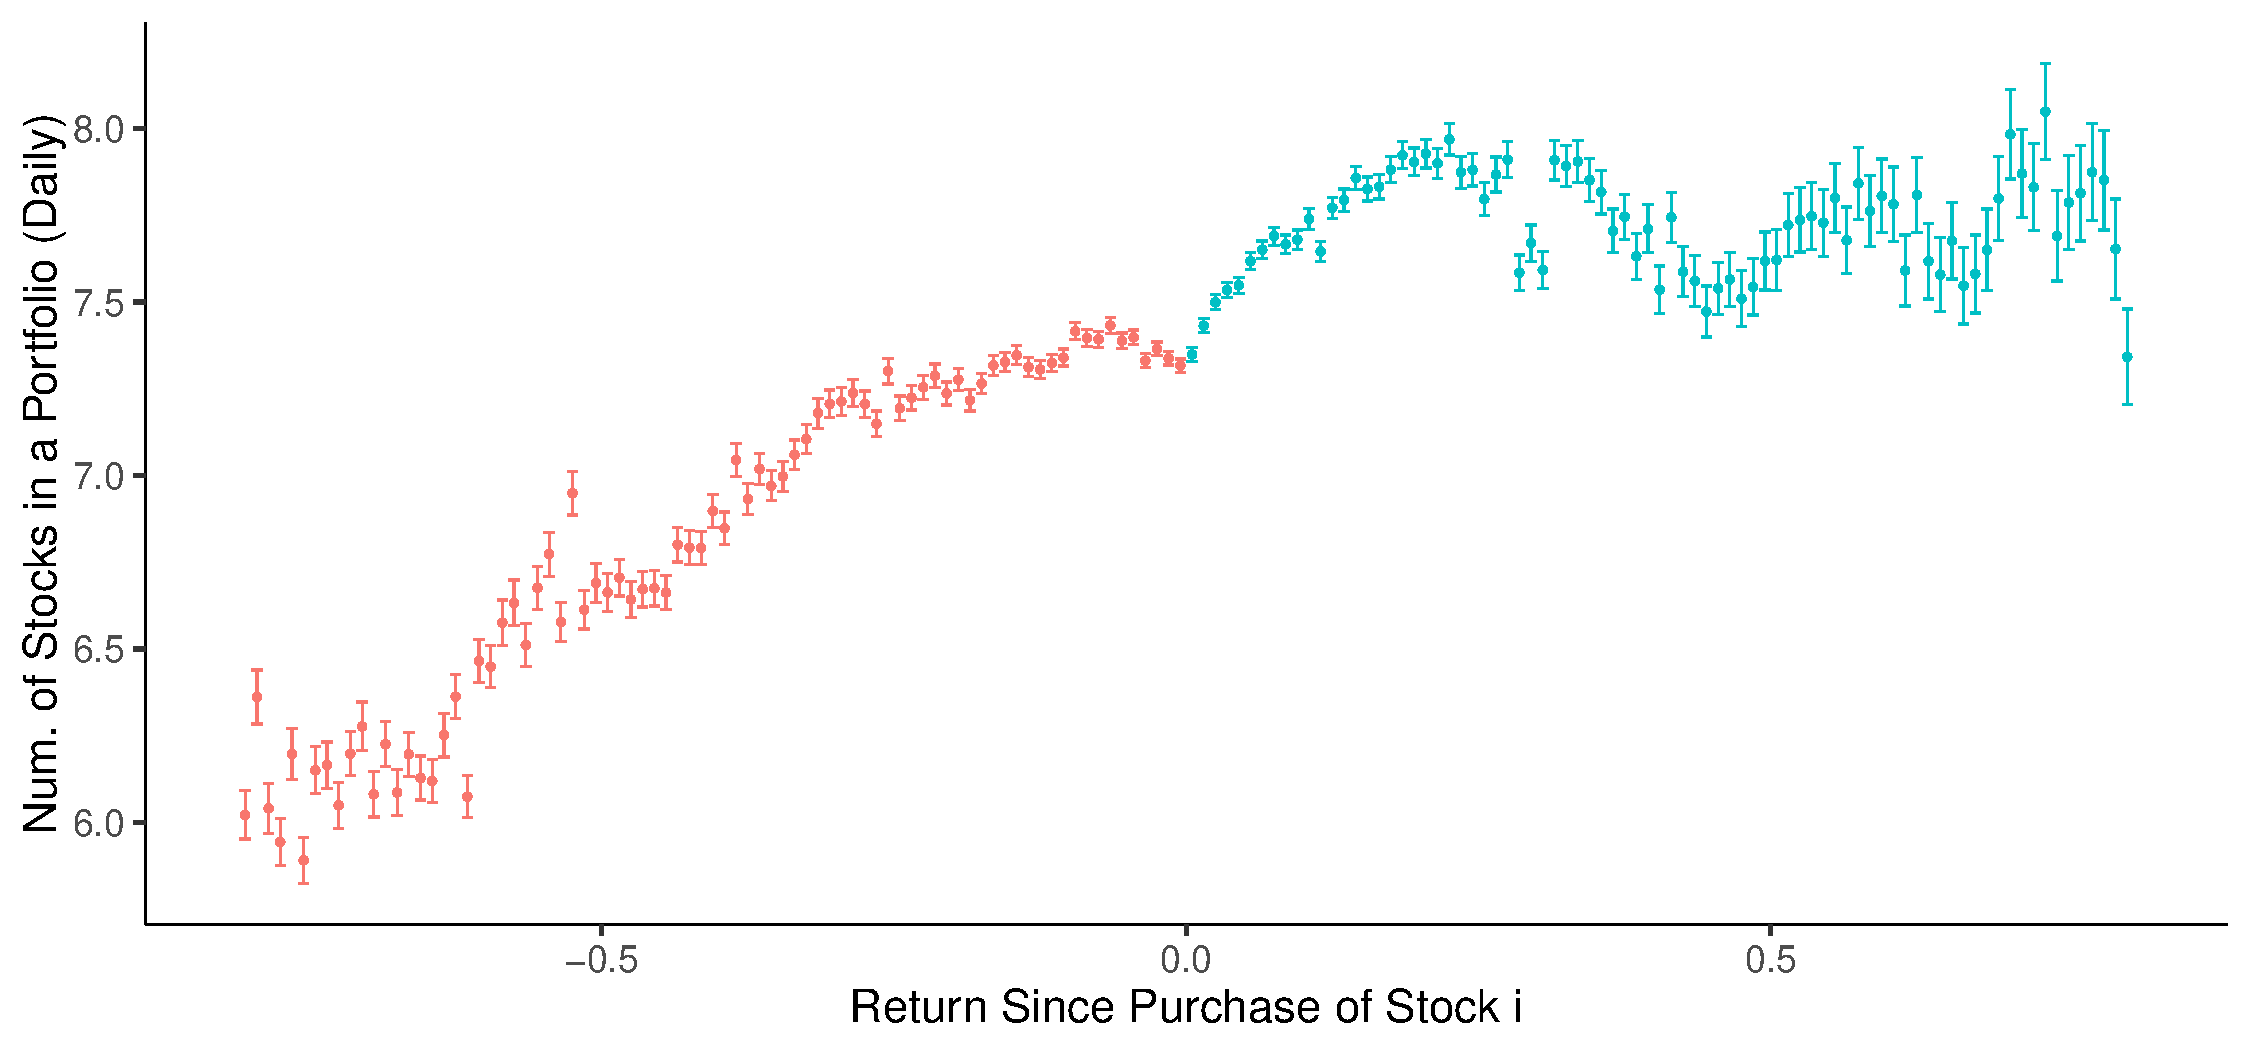
\includegraphics[width=0.8\columnwidth]{barc_num_stocks_daily_N2_3.pdf}
	\caption{\small Number of stocks in a portfolio on return since purchase (Daily portfolio sample given $N\geq2$)}
	\label{figure:N_on_return_n2}
\end{figure}

\begin{figure}[H]
	\centering
	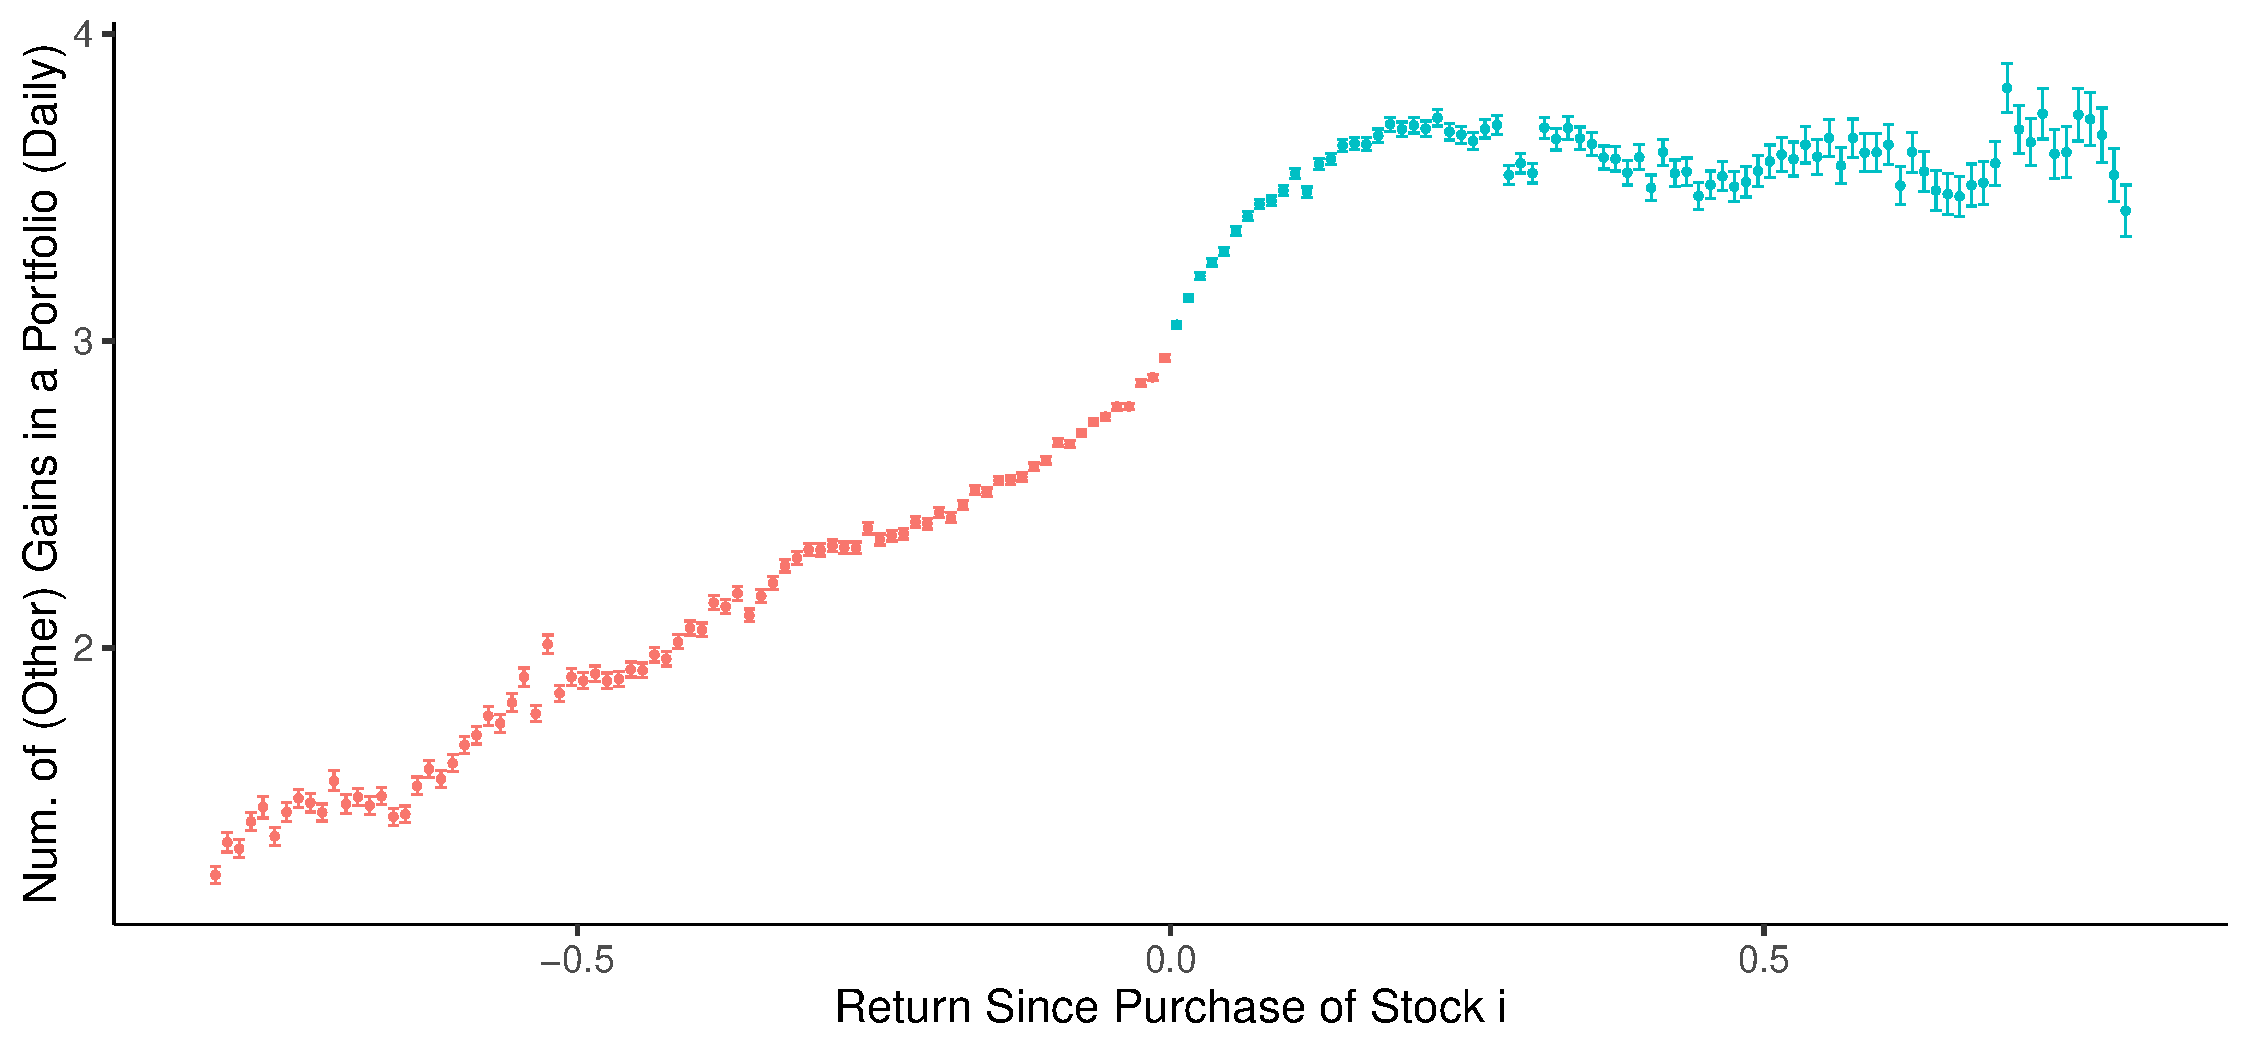
\includegraphics[width=0.8\columnwidth]{barc_NG_daily_N2_3.pdf}
	\caption{\small Number of gains in a portfolio on return since purchase (Daily portfolio sample given $N\geq2$). One gain was not counted in the gain domain.}
	\label{figure:NG_on_return_n2}
\end{figure}

\begin{figure}[H]
	\centering
	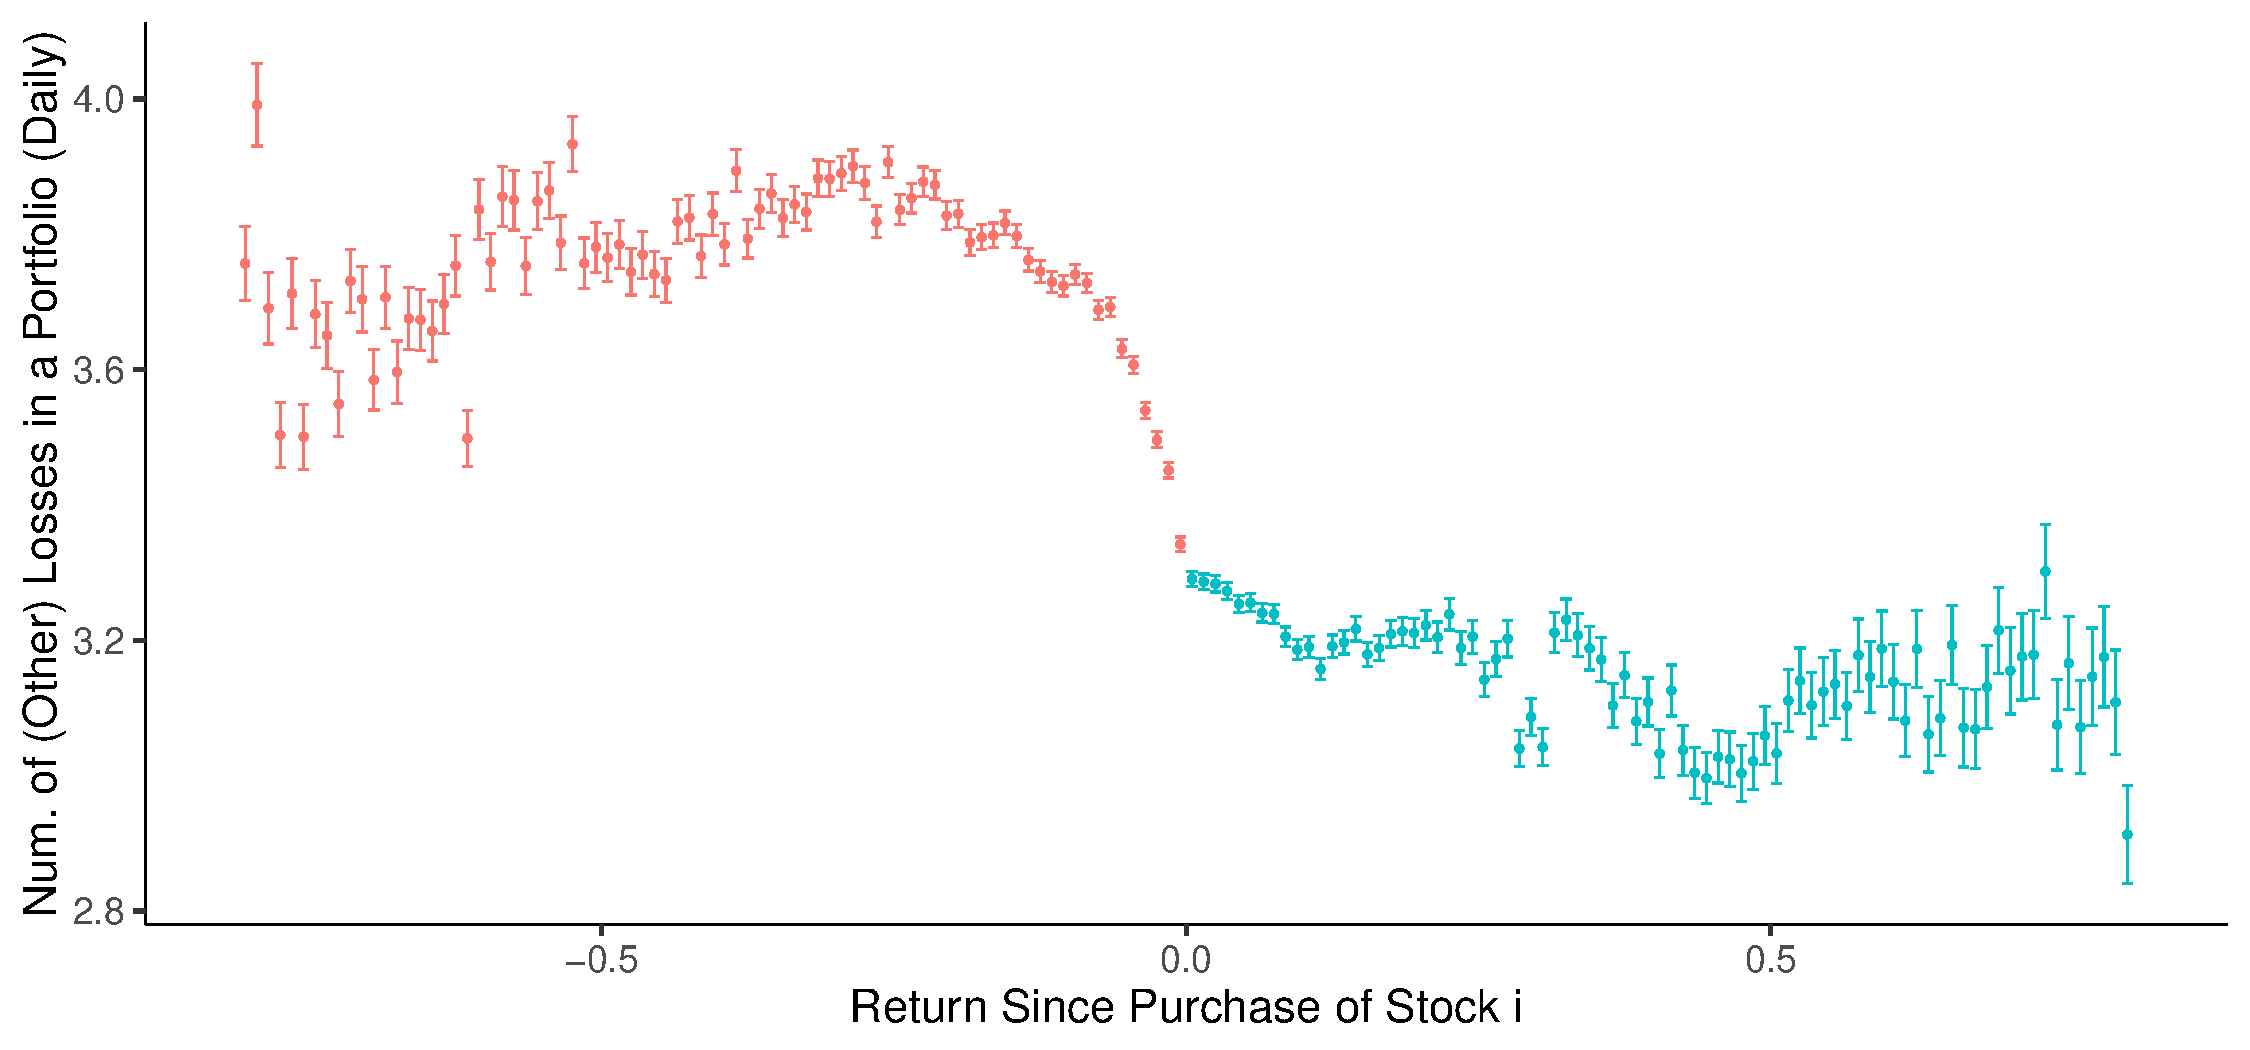
\includegraphics[width=0.8\columnwidth]{barc_NL_daily_N2_3.pdf}
	\caption{\small Number of losses in a portfolio on return since purchase (Daily portfolio sample given $N\geq2$). One loss was not counted in the loss domain.}
	\label{figure:NL_on_return_n2}
\end{figure}

\pagebreak

\begin{figure}[H]
	\centering
	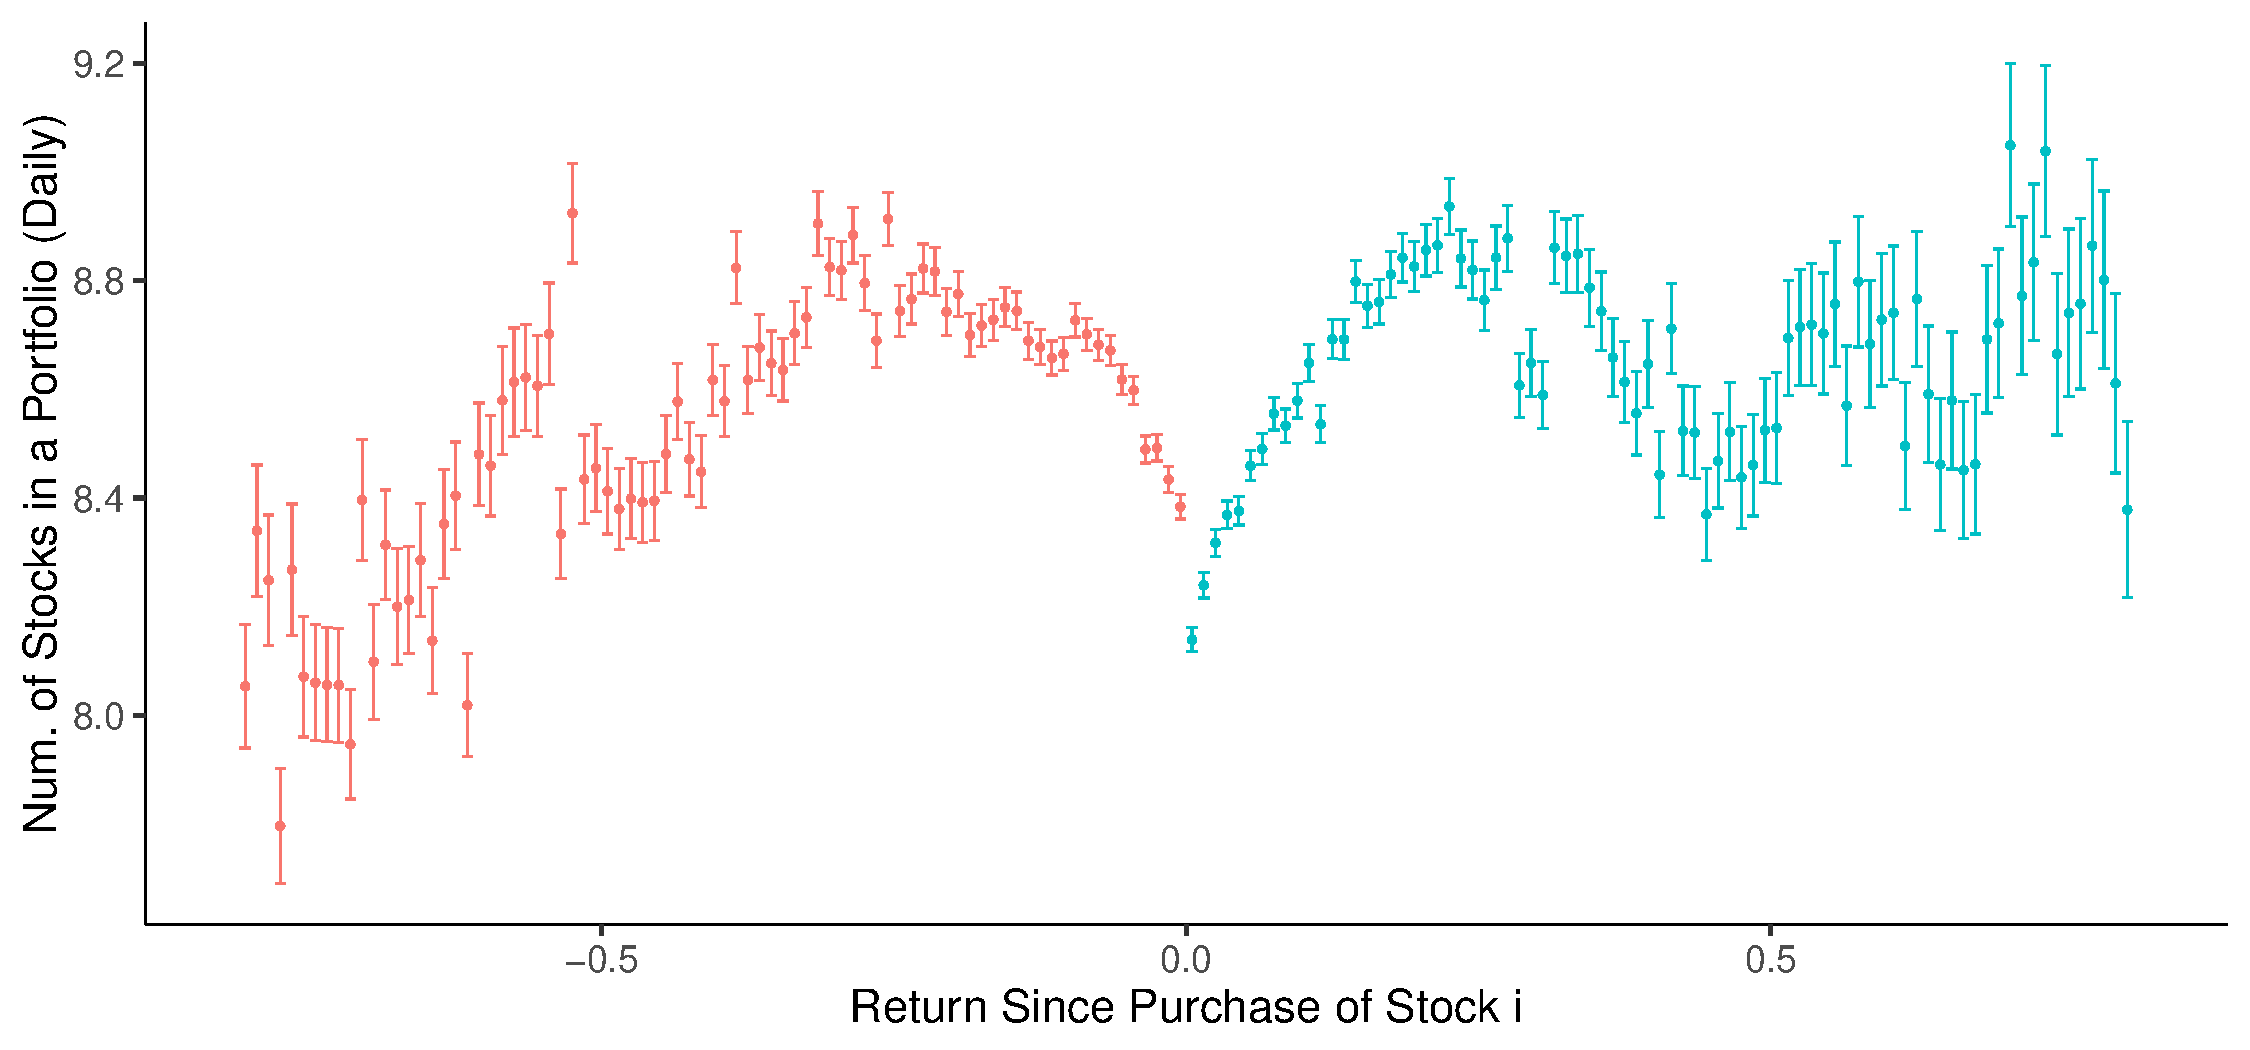
\includegraphics[width=0.8\columnwidth]{barc_num_stocks_daily_NG1_NL1_3.pdf}
	\caption{\small Number of stocks in a portfolio on return since purchase (Daily portfolio sample given$NG\geq1$ and $NL\geq1$)}
	\label{figure:N_on_return_ng1_nl1}
\end{figure}


\begin{figure}[H]
	\centering
	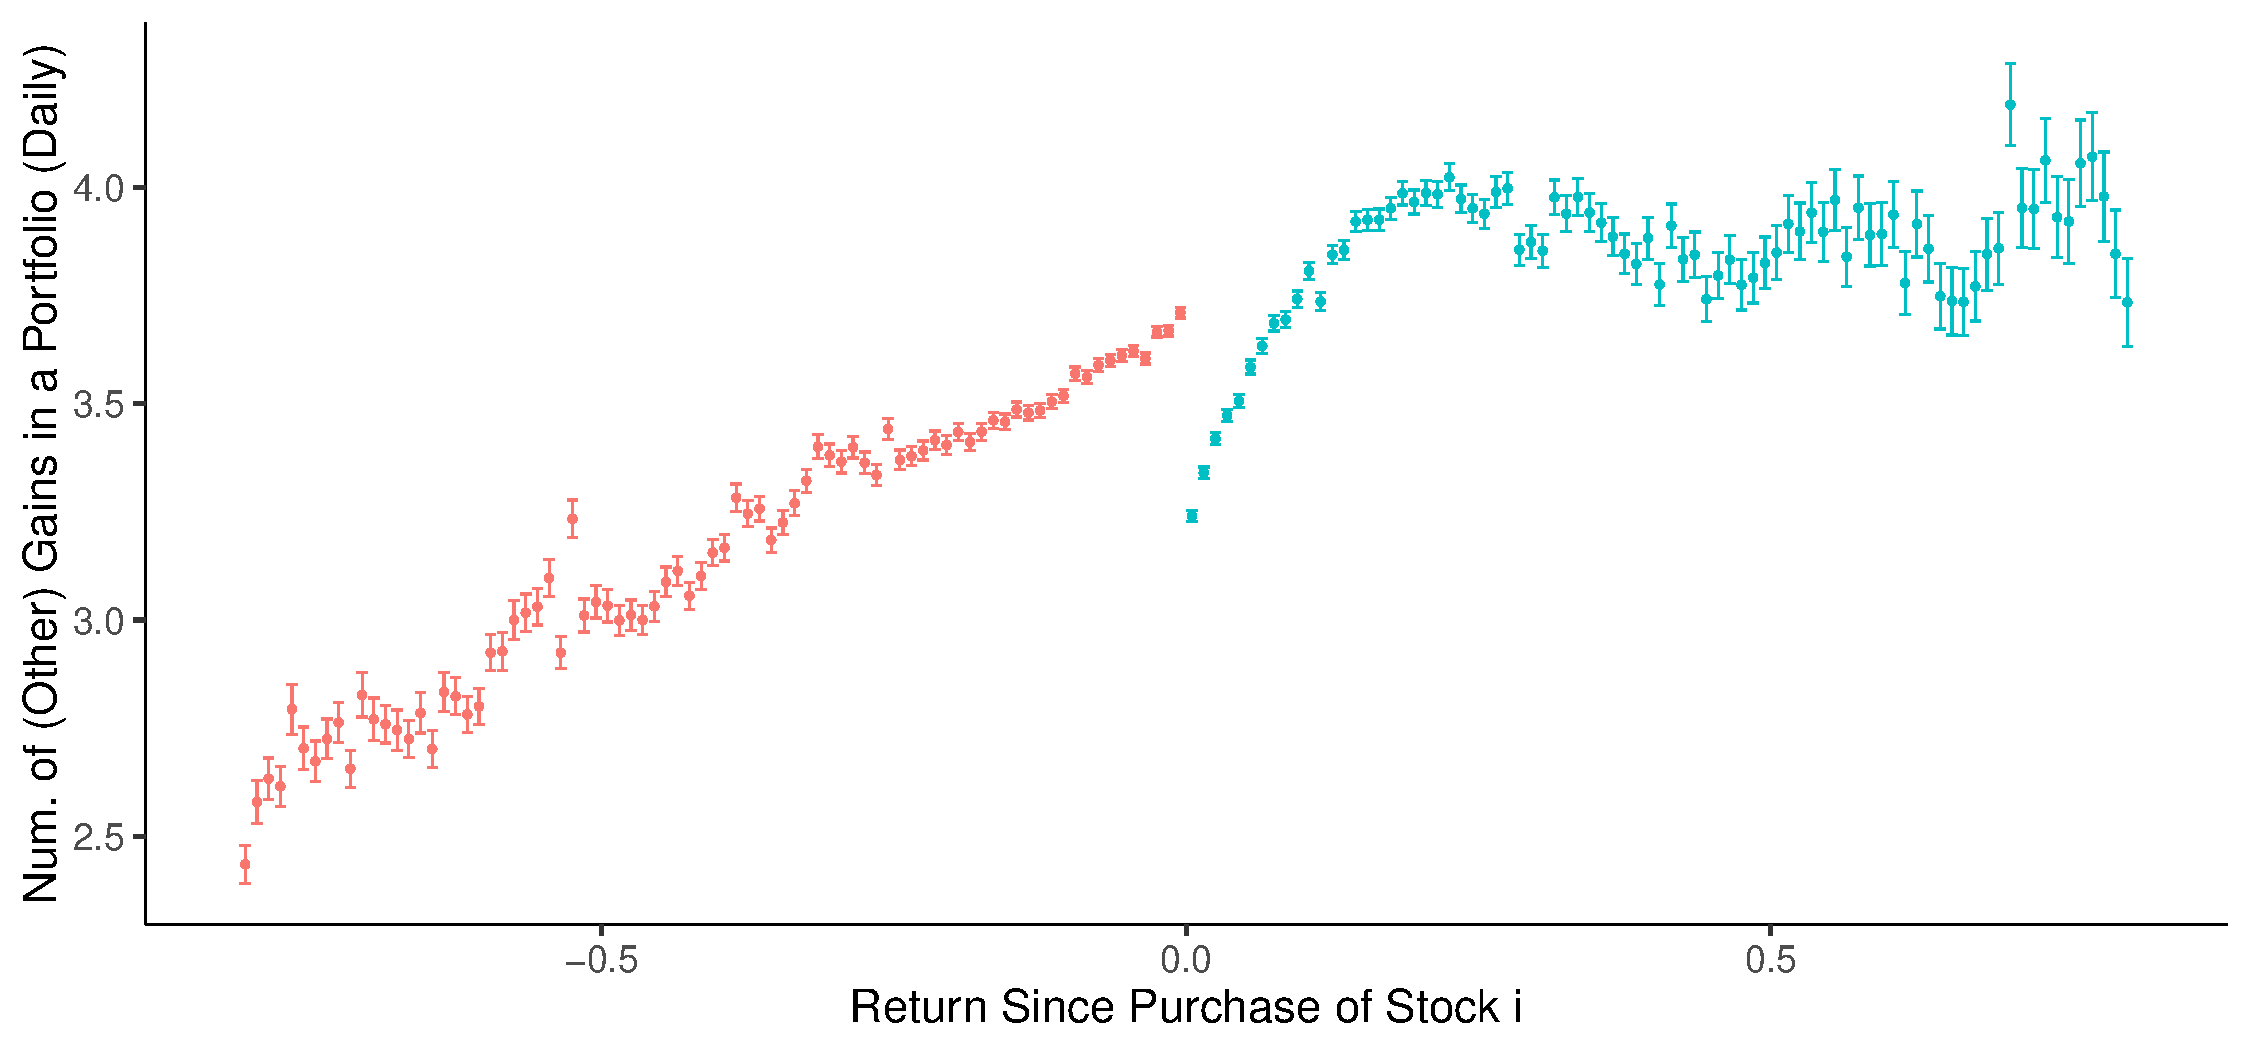
\includegraphics[width=0.8\columnwidth]{barc_NG_daily_NG1_NL1_3.pdf}
	\caption{\small Number of gains in a portfolio on return since purchase (Daily portfolio sample given $NG\geq1$ and $NL\geq1$). One gain was not counted in the gain domain.}
	\label{figure:NG_on_return_ng1_nl1}
\end{figure}

\begin{figure}[H]
	\centering
	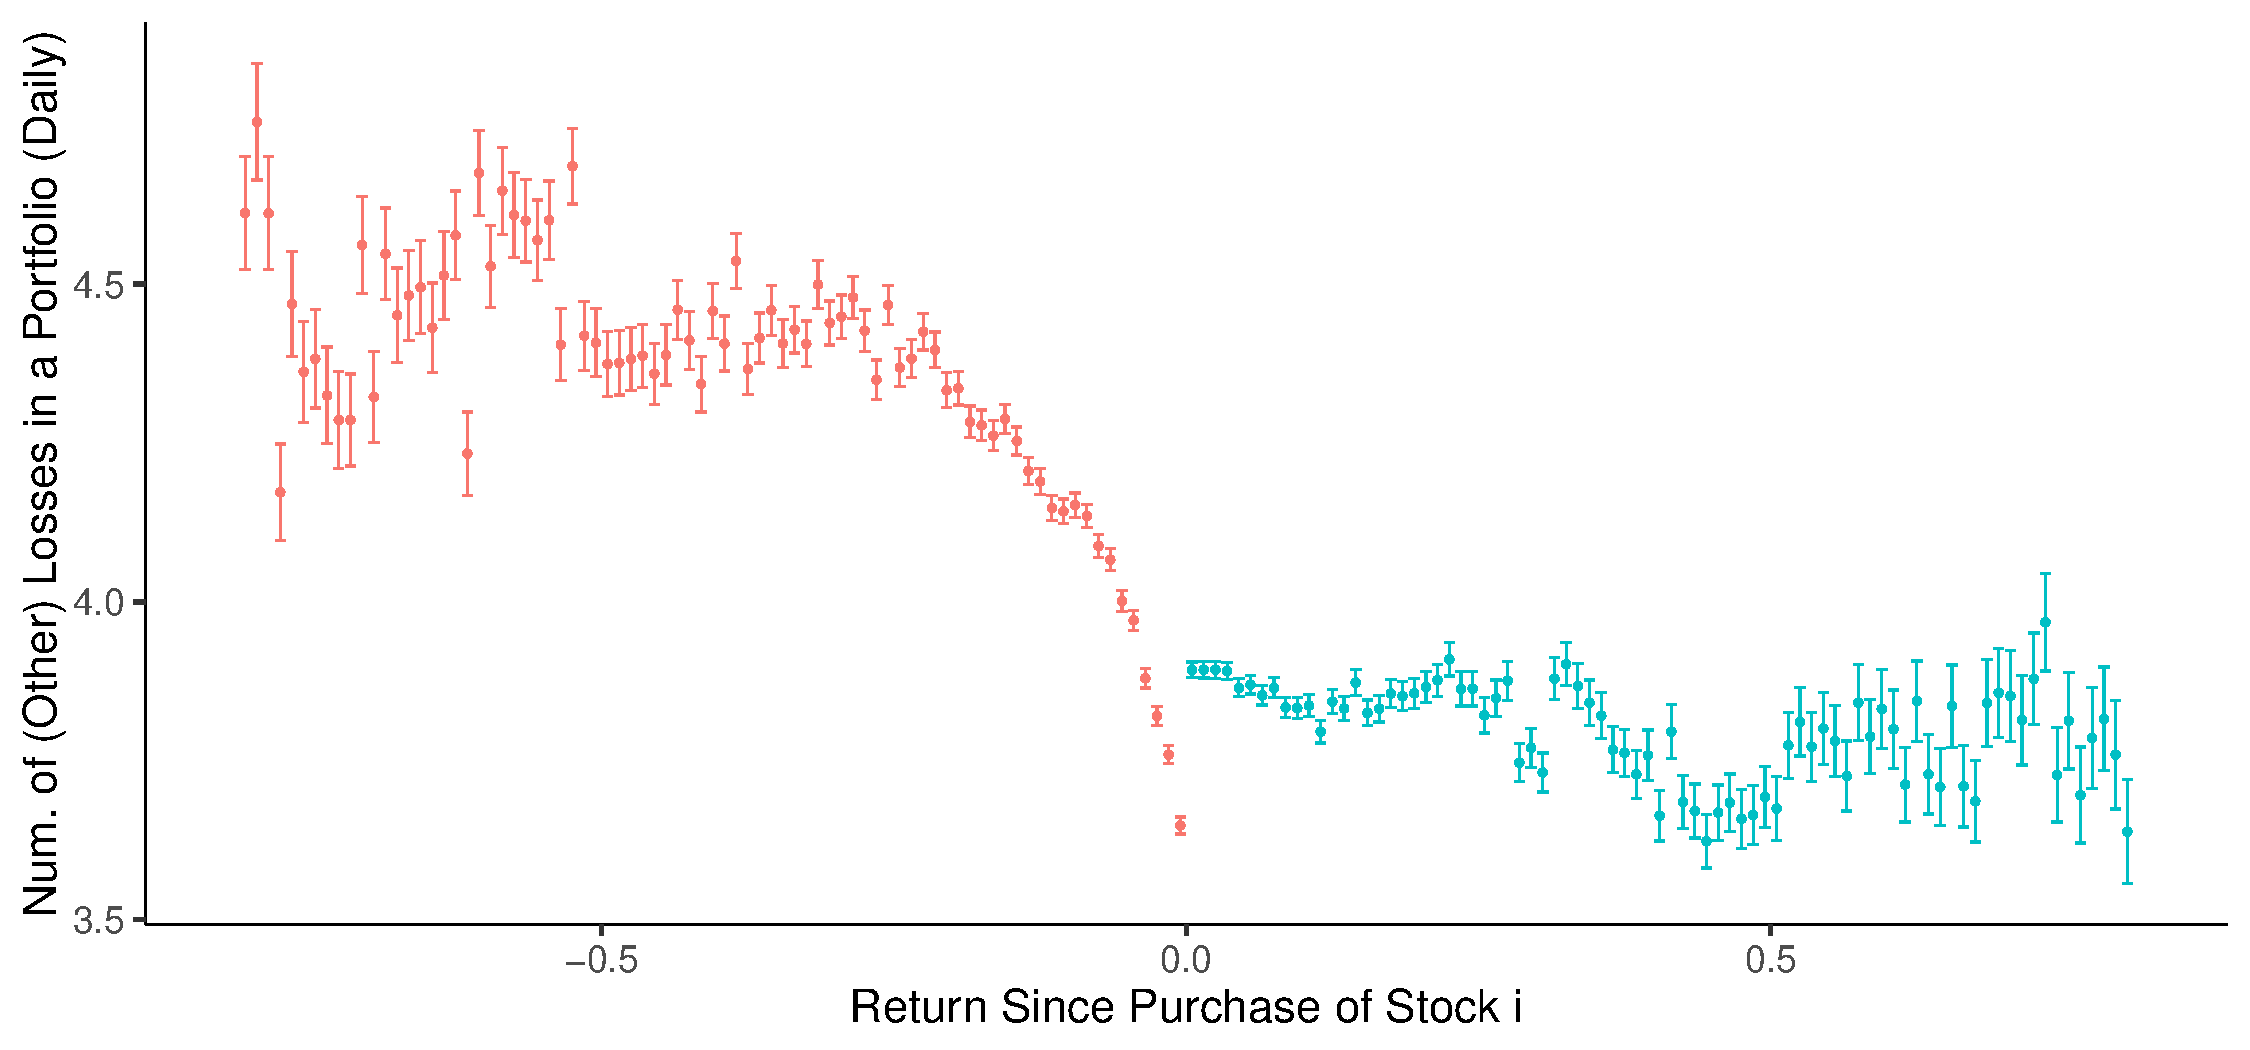
\includegraphics[width=0.8\columnwidth]{barc_NL_daily_NG1_NL1_3.pdf}
	\caption{\small Number of losses in a portfolio on return since purchase (Daily portfolio sample given $NG\geq1$ and $NL\geq1$). One loss was not counted in the loss domain.}
	\label{figure:NL_on_return_ng1_nl1}
\end{figure}


\begin{figure}[H]
	\centering
	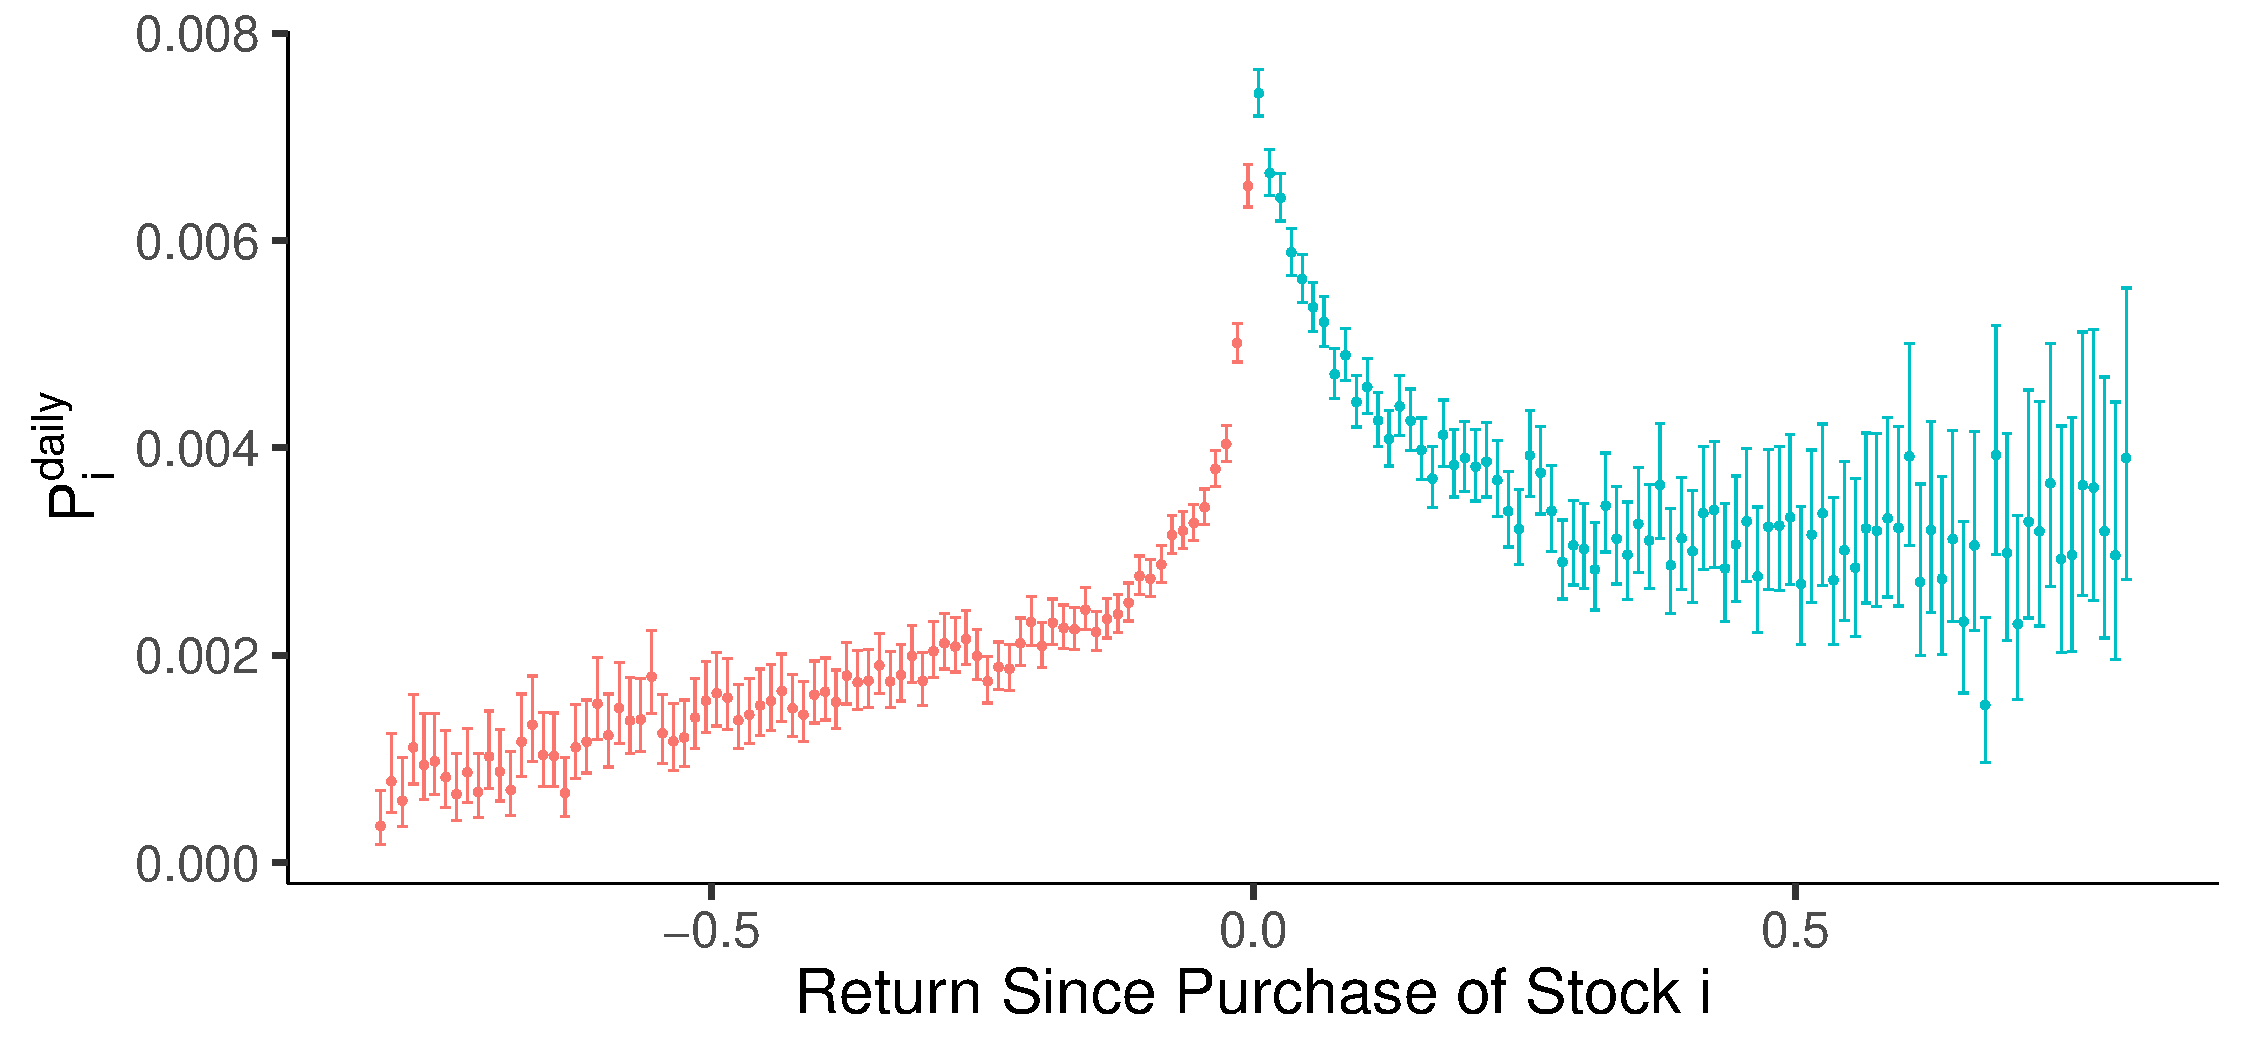
\includegraphics[width=0.8\columnwidth]{barc_schedule_daily_N2_3.pdf}
	\caption{Proportion of stocks being sold ($P^{daily}_{i}$; Daily portfolio sample given $N\geq2$). The bin-width is 0.01. The error bars are 95\% confidence intervals.}
	\label{figure:prop_n2}
\end{figure}

\begin{figure}[H]
	\centering
	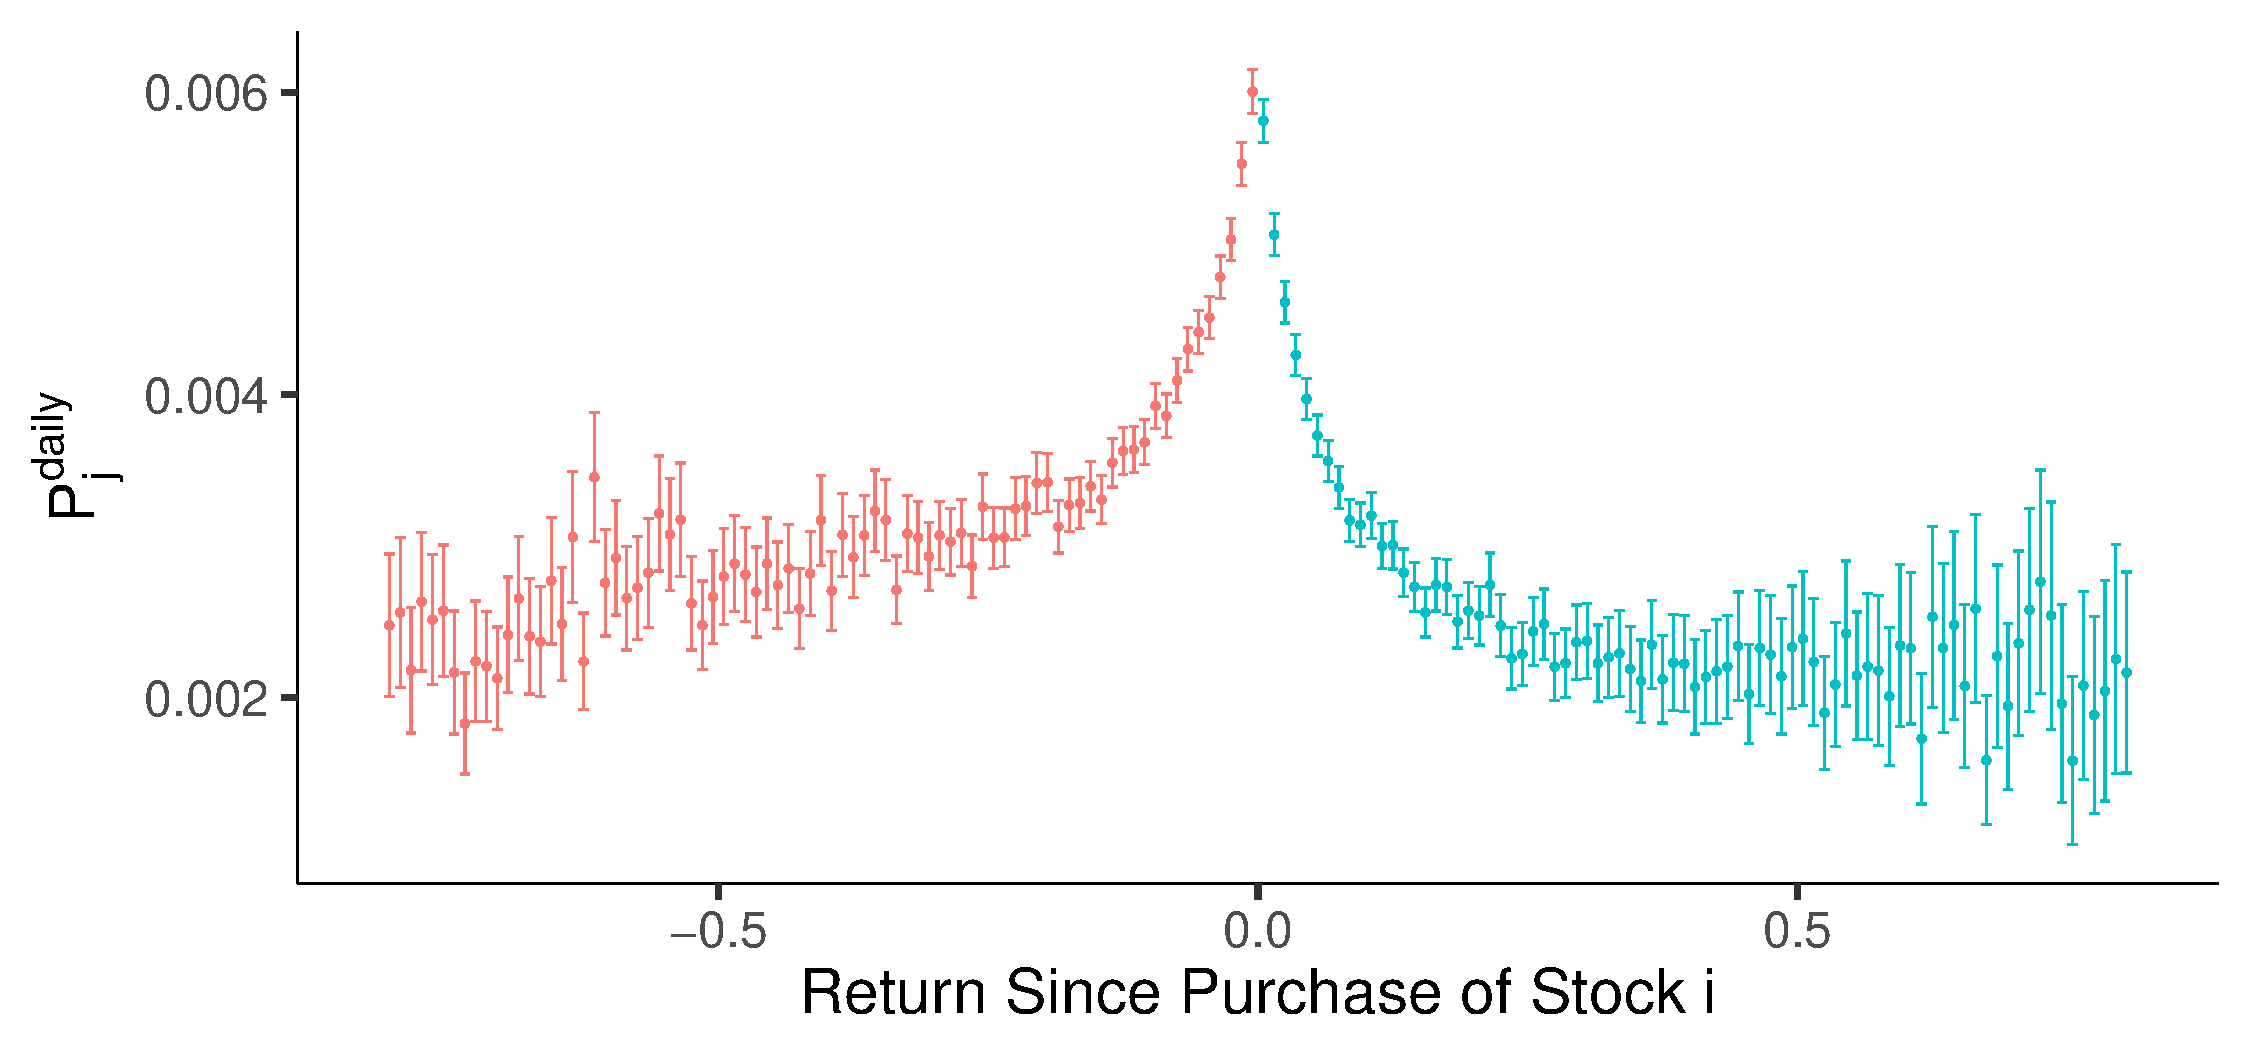
\includegraphics[width=0.8\columnwidth]{barc_other_sold_daily_3.pdf}
	\caption{Proportion of other stocks in the portfolios being sold ($P^{daily}_{j}$; Daily portfolio sample given $N\geq2$). The bin-width is 0.01. The error bars are 95\% confidence intervals.}
	\label{figure:prop_others_n2}
\end{figure}



\begin{figure}[H]
	\centering
	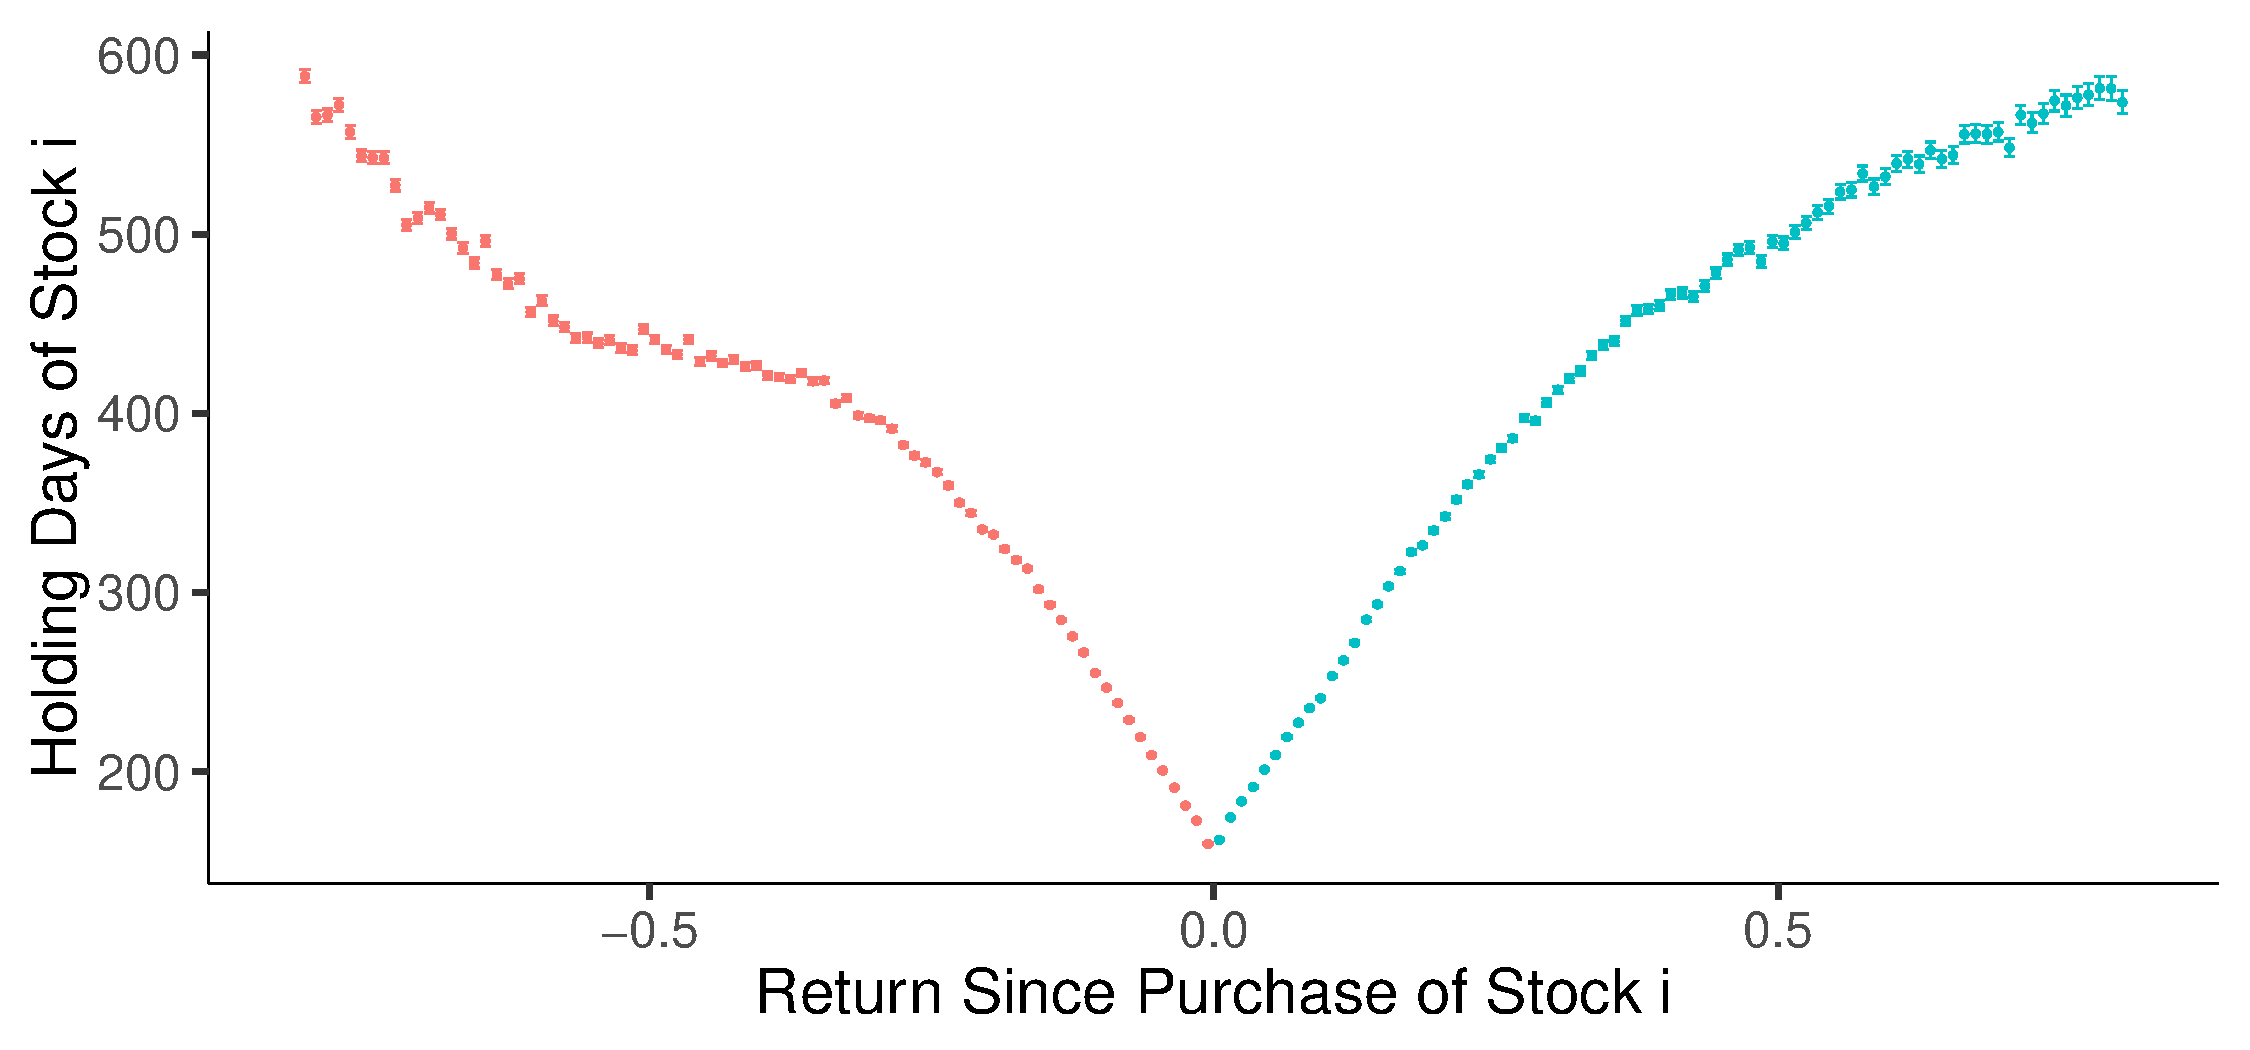
\includegraphics[width=0.8\columnwidth]{barc_holding_days_daily_N2_3.pdf}
	\caption{Holding Days of Stock $i$ (Daily portfolio sample given $N\geq2$). The bin-width is 0.01. The error bars are 95\% confidence intervals.}
	\label{figure:holding_days_n2}
\end{figure}

\begin{figure}[H]
	\centering
	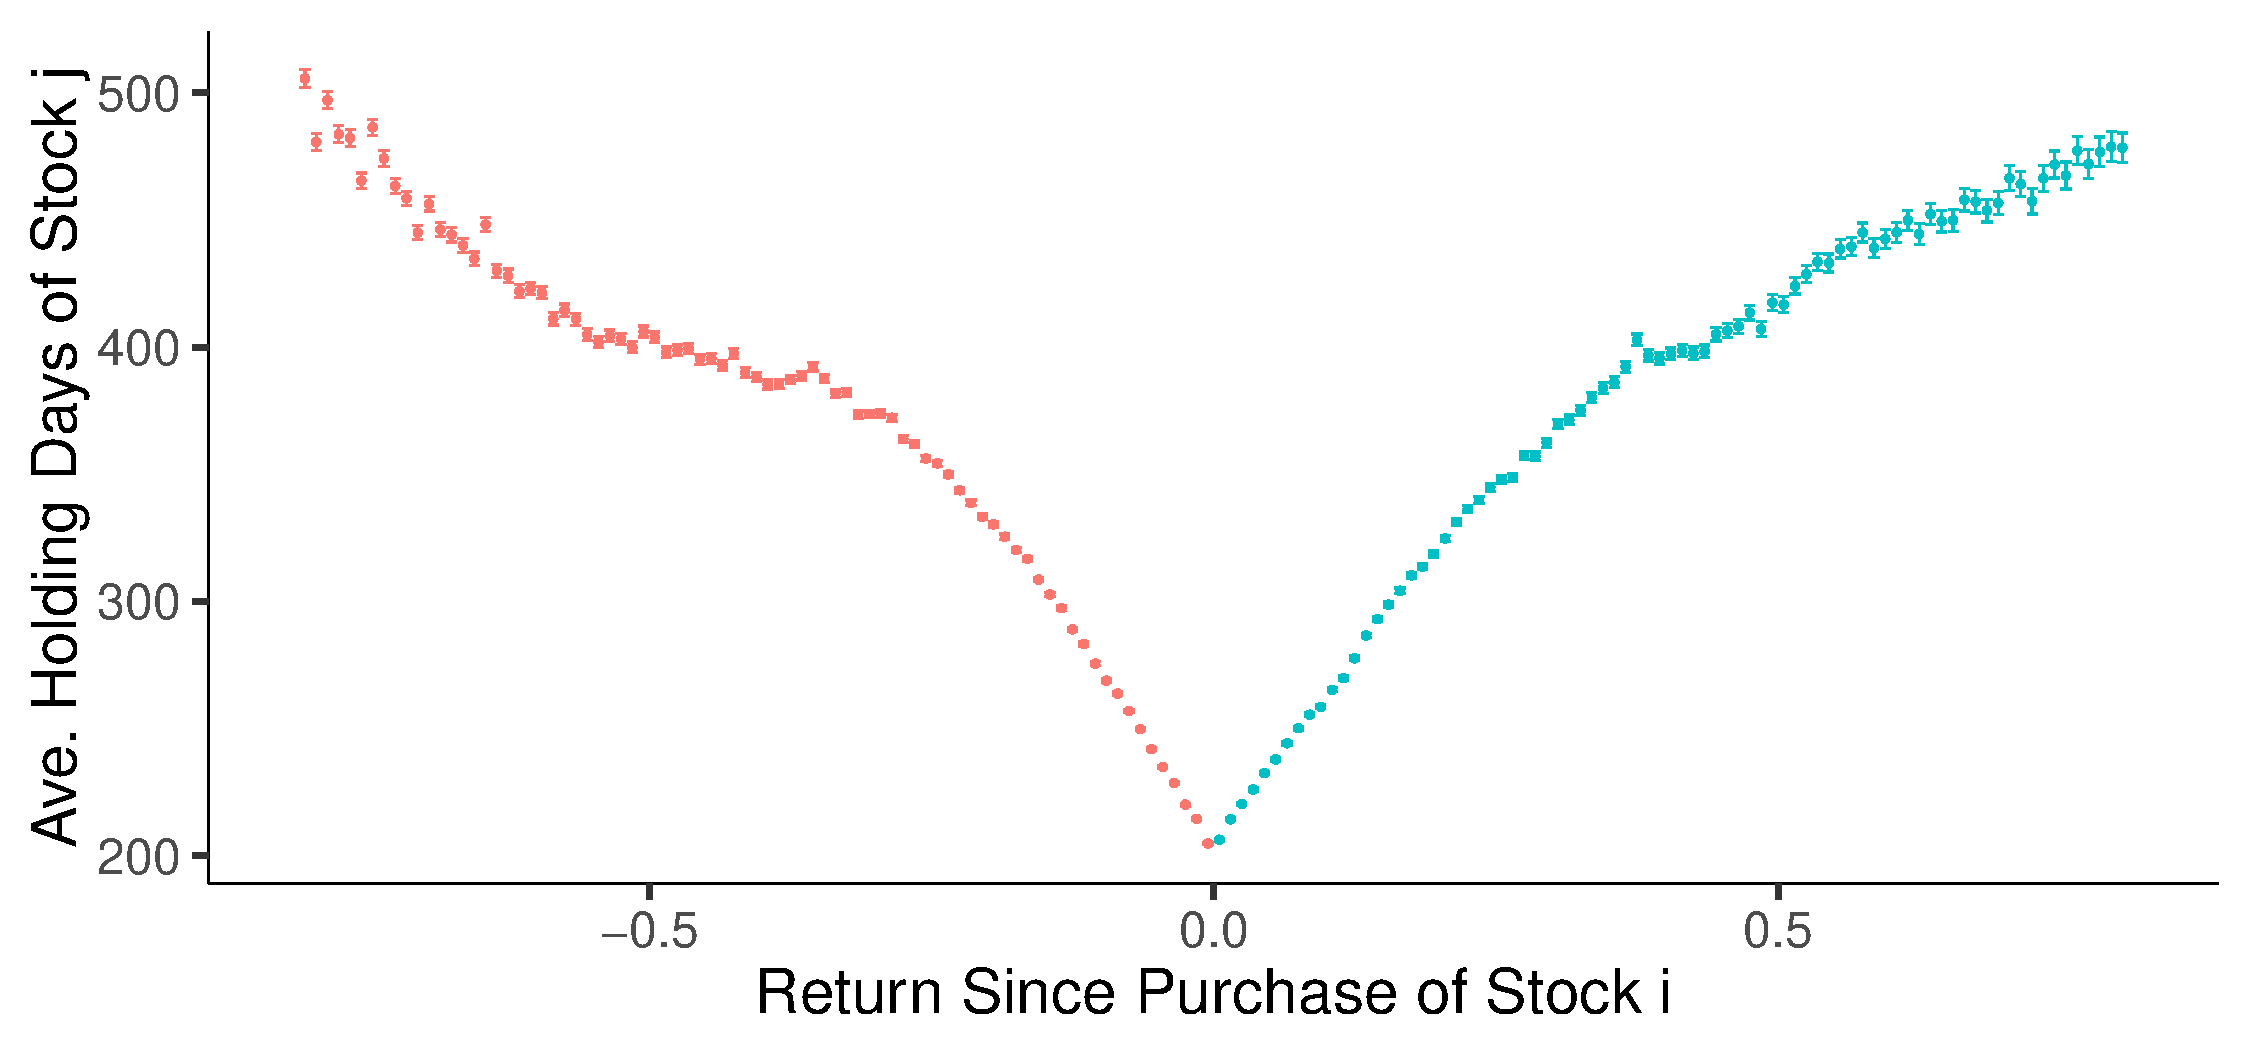
\includegraphics[width=0.8\columnwidth]{barc_holding_days_others_daily_N2_3.pdf}
	\caption{Average Holding Days of Stock $j$ (Daily portfolio sample given $N\geq2$). The bin-width is 0.01. The error bars are 95\% confidence intervals.}
	\label{figure:holding_days_others_n2}
\end{figure}


\begin{figure}[H]
	\centering
	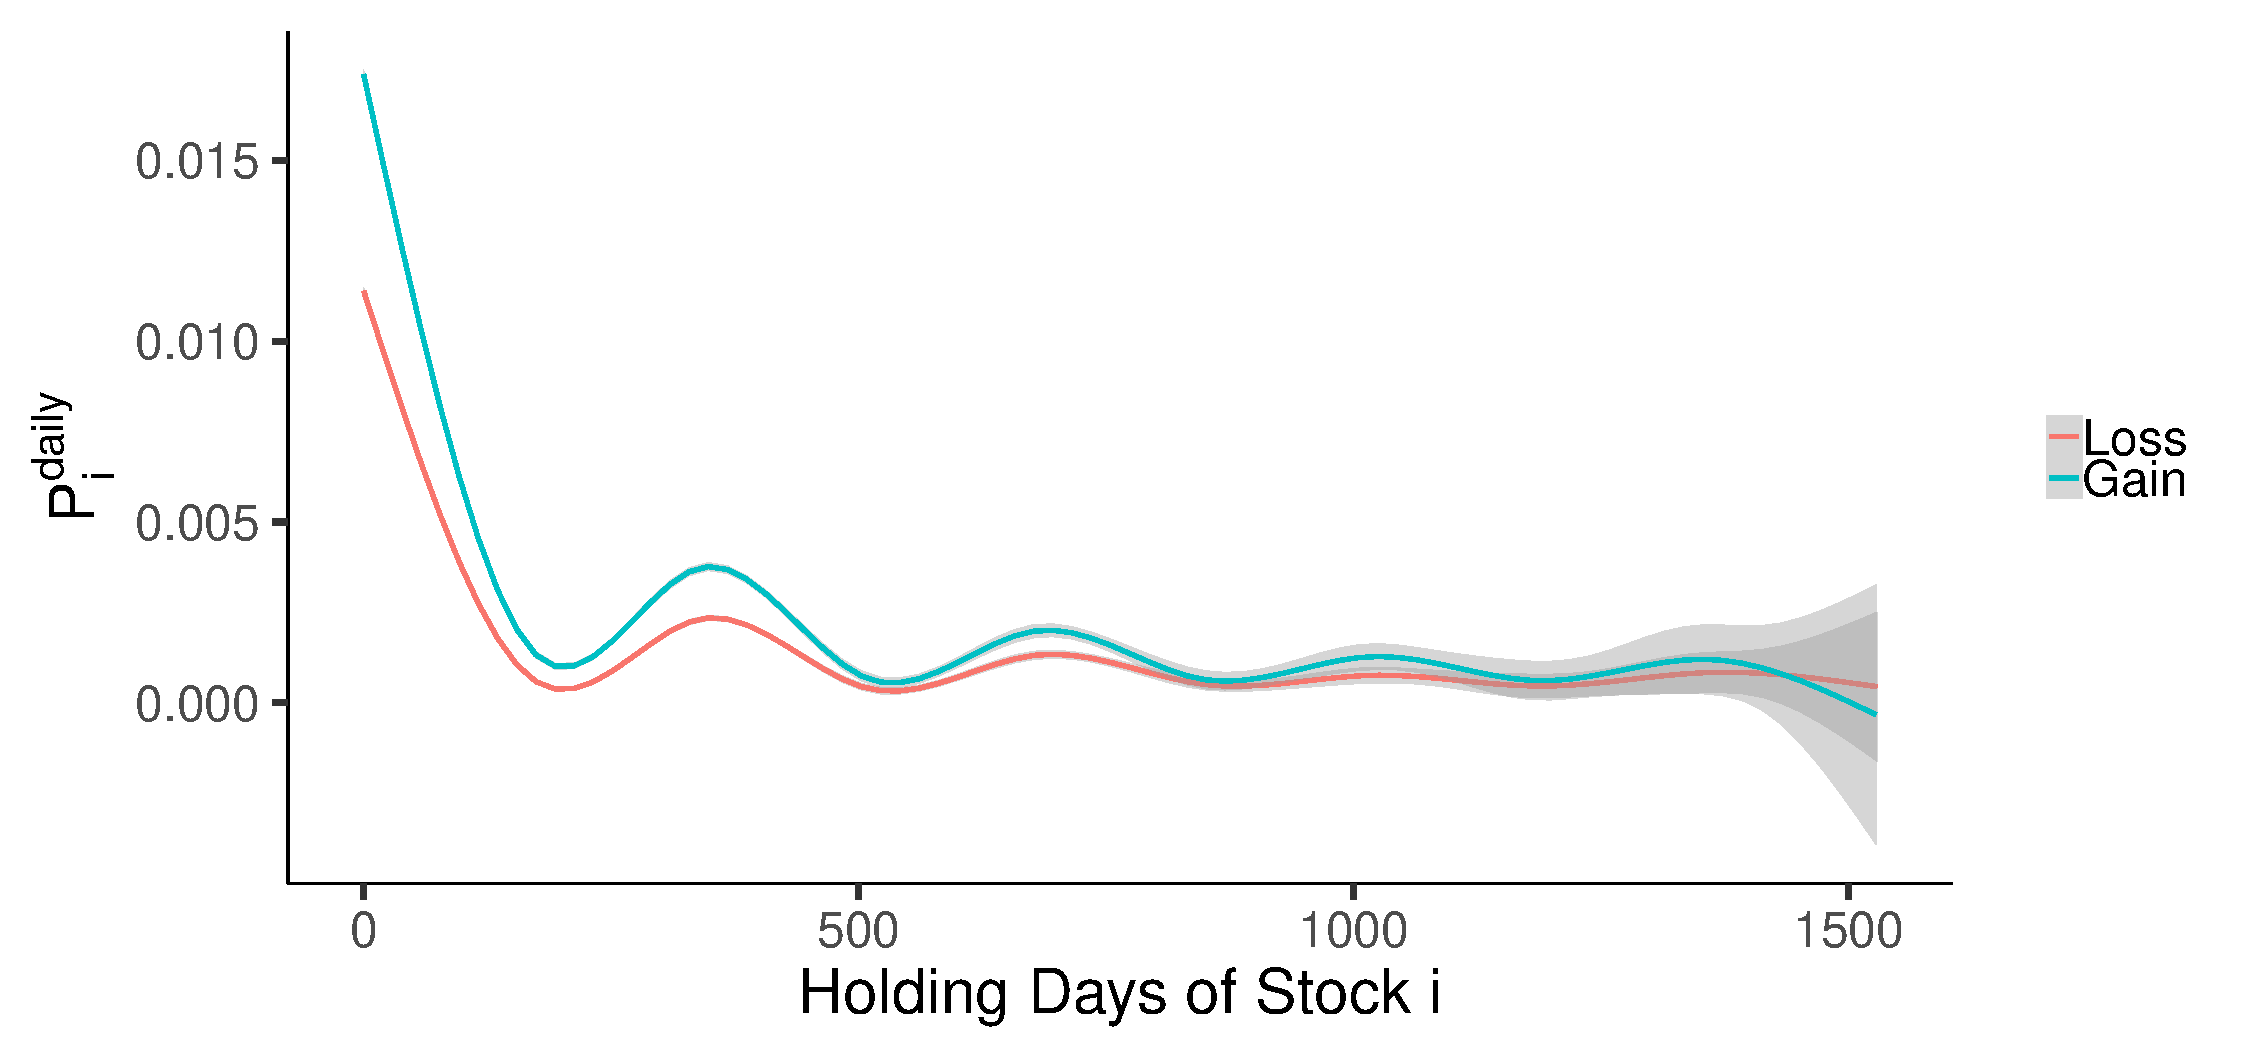
\includegraphics[width=0.8\columnwidth]{barc_schedule_on_holding_days.pdf}
	\caption{$P^{daily}_{i}$ on Holding Period (Daily portfolio sample).}
	\label{figure:schedule_holding_days}
\end{figure}

\begin{figure}[H]
	\centering
	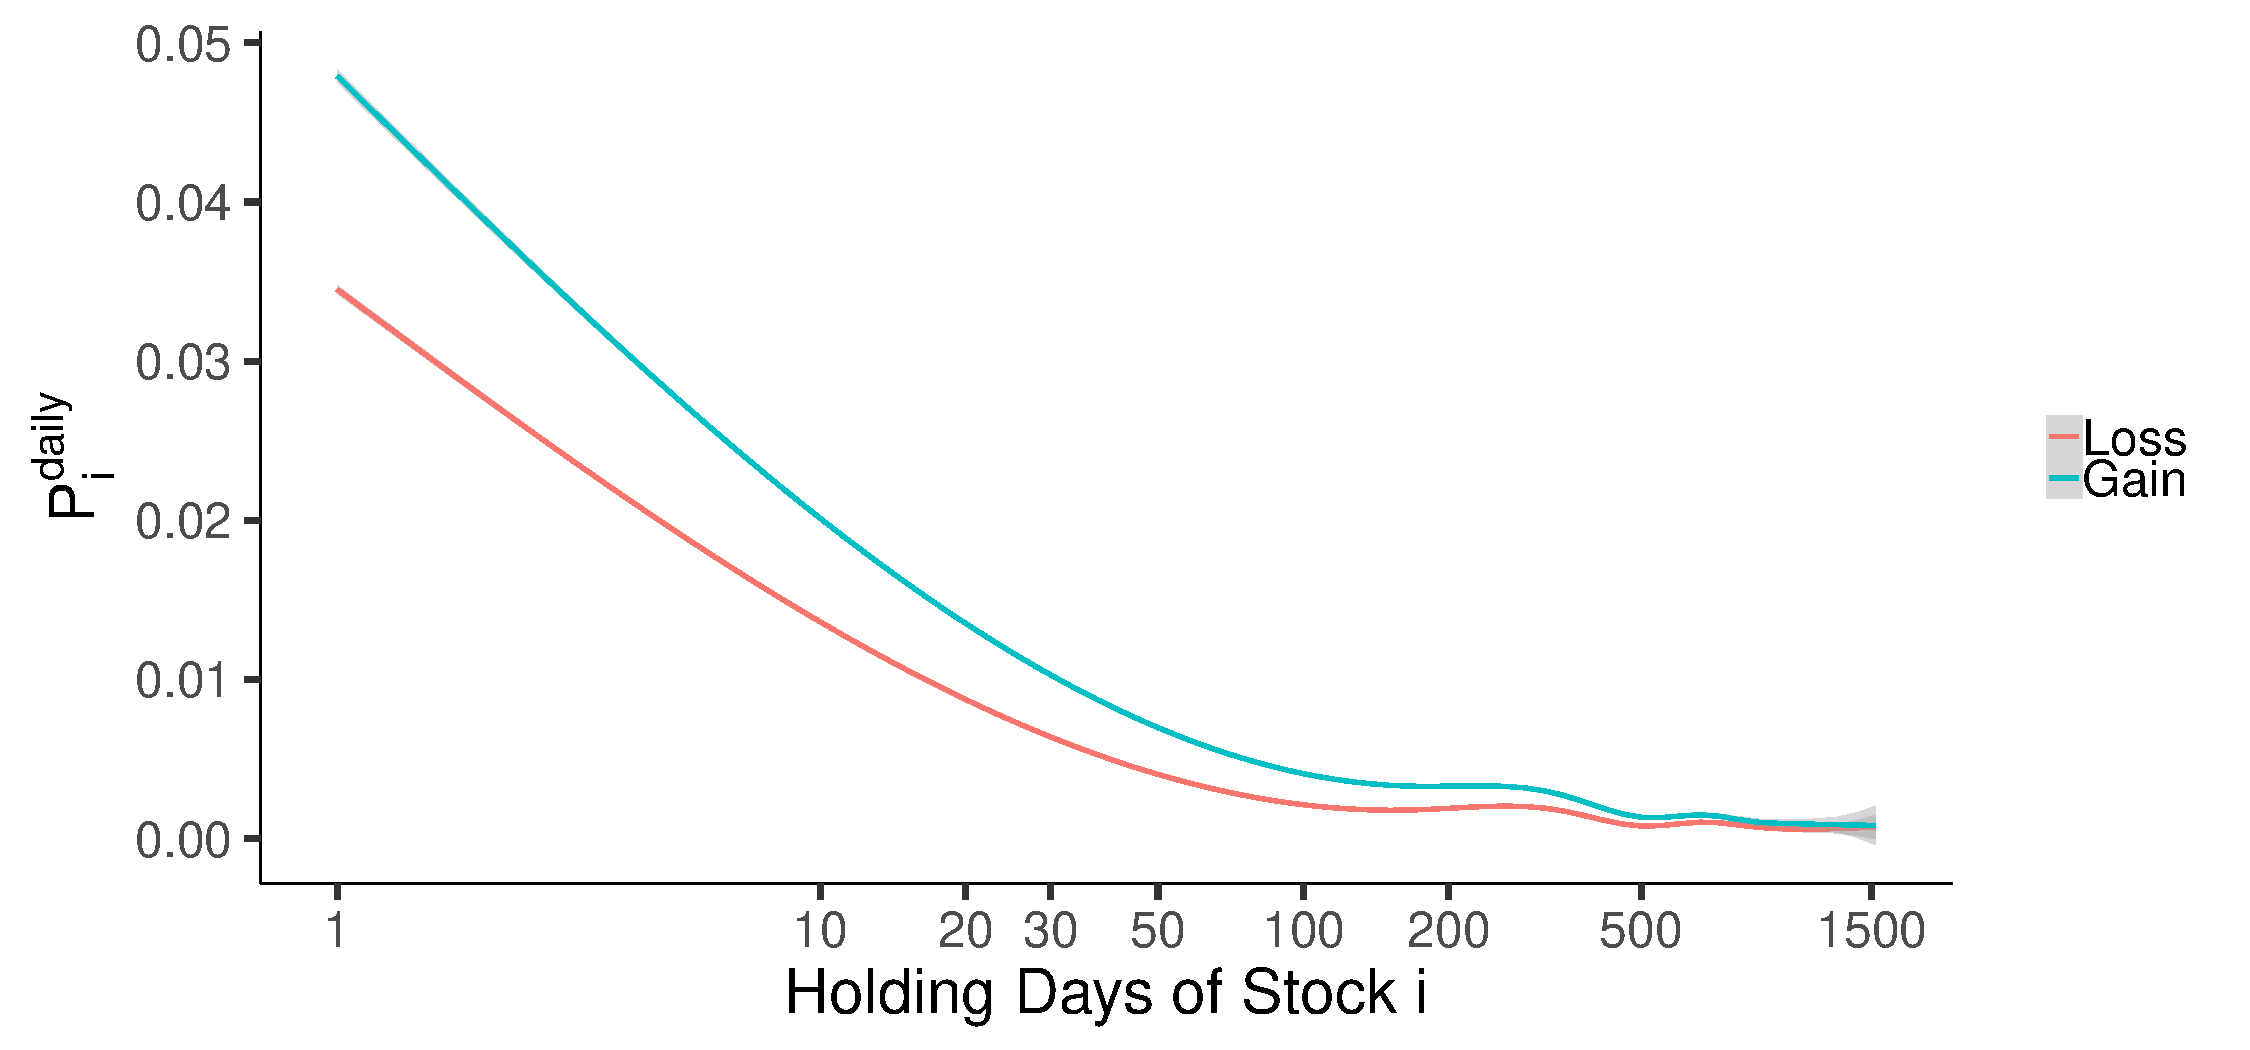
\includegraphics[width=0.8\columnwidth]{barc_schedule_on_holding_days_log.pdf}
	\caption{$P^{daily}_{i}$ on Holding Period (Daily portfolio sample). The x-axis are log transformed.}
	\label{figure:schedule_holding_days_log}
\end{figure}


\begin{figure}[H]
	\centering
	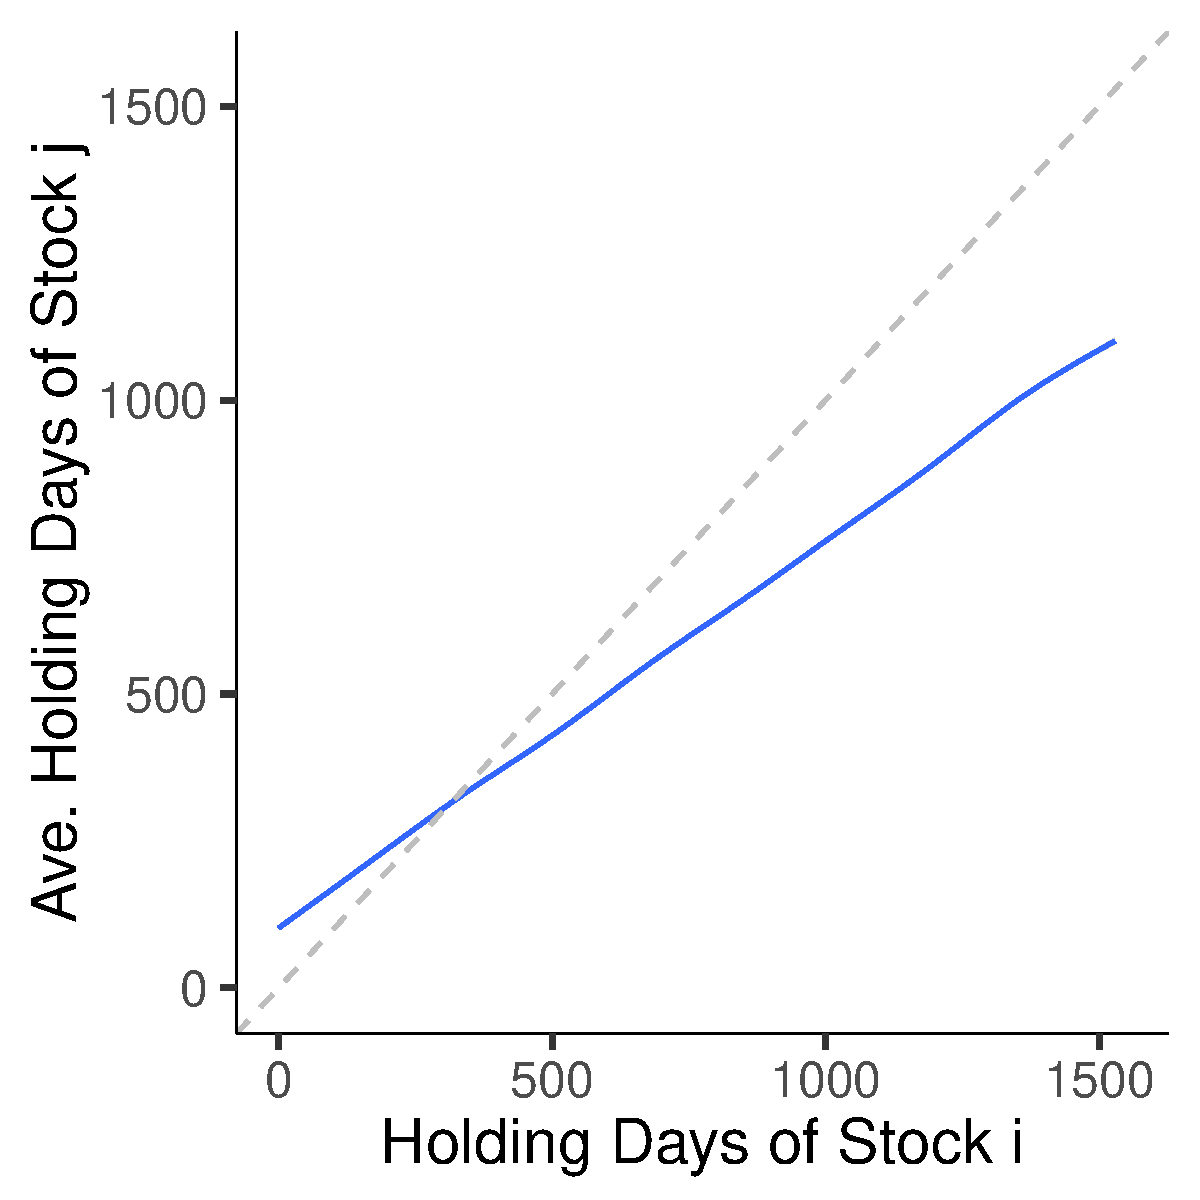
\includegraphics[width=0.6\columnwidth]{barc_holding_days_i_j.pdf}
	\caption{Holding Periods of Stock $i$ and Average Holding Period of Stocks $j$.}
	\label{figure:holding_days_i_j}
\end{figure}


\begin{figure}[H]
	\centering
	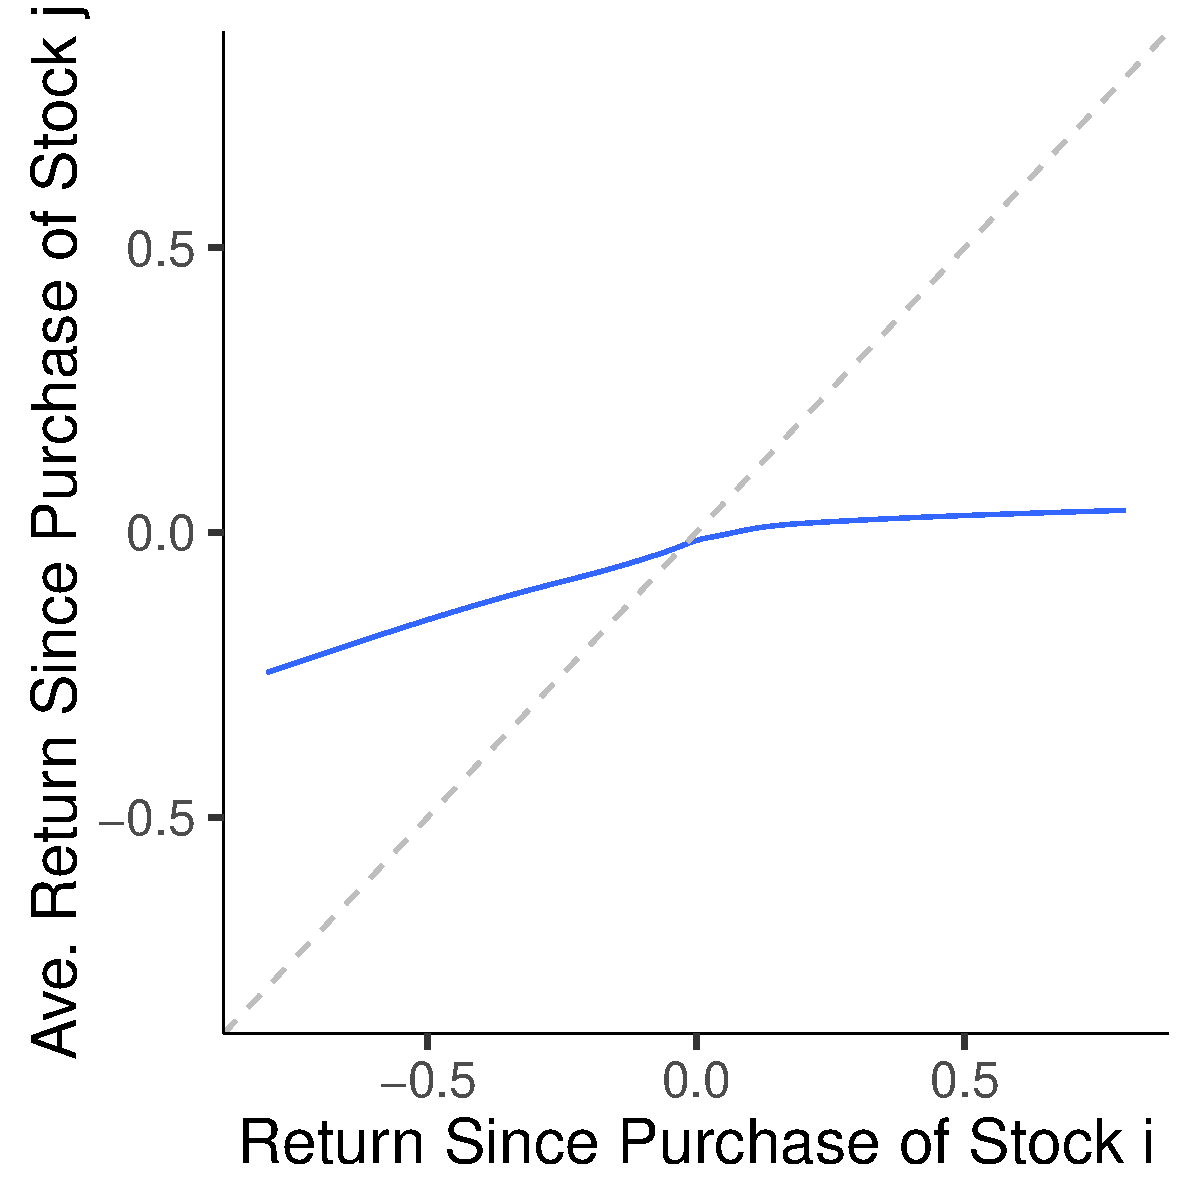
\includegraphics[width=0.6\columnwidth]{barc_R_i_R_j.pdf}
	\caption{Return of stock $i$ and average return of stocks $j$ (Daily portfolio sample given $N\geq2$).}
	\label{figure:ret_i_j}
\end{figure}

\begin{figure}[H]
	\centering
	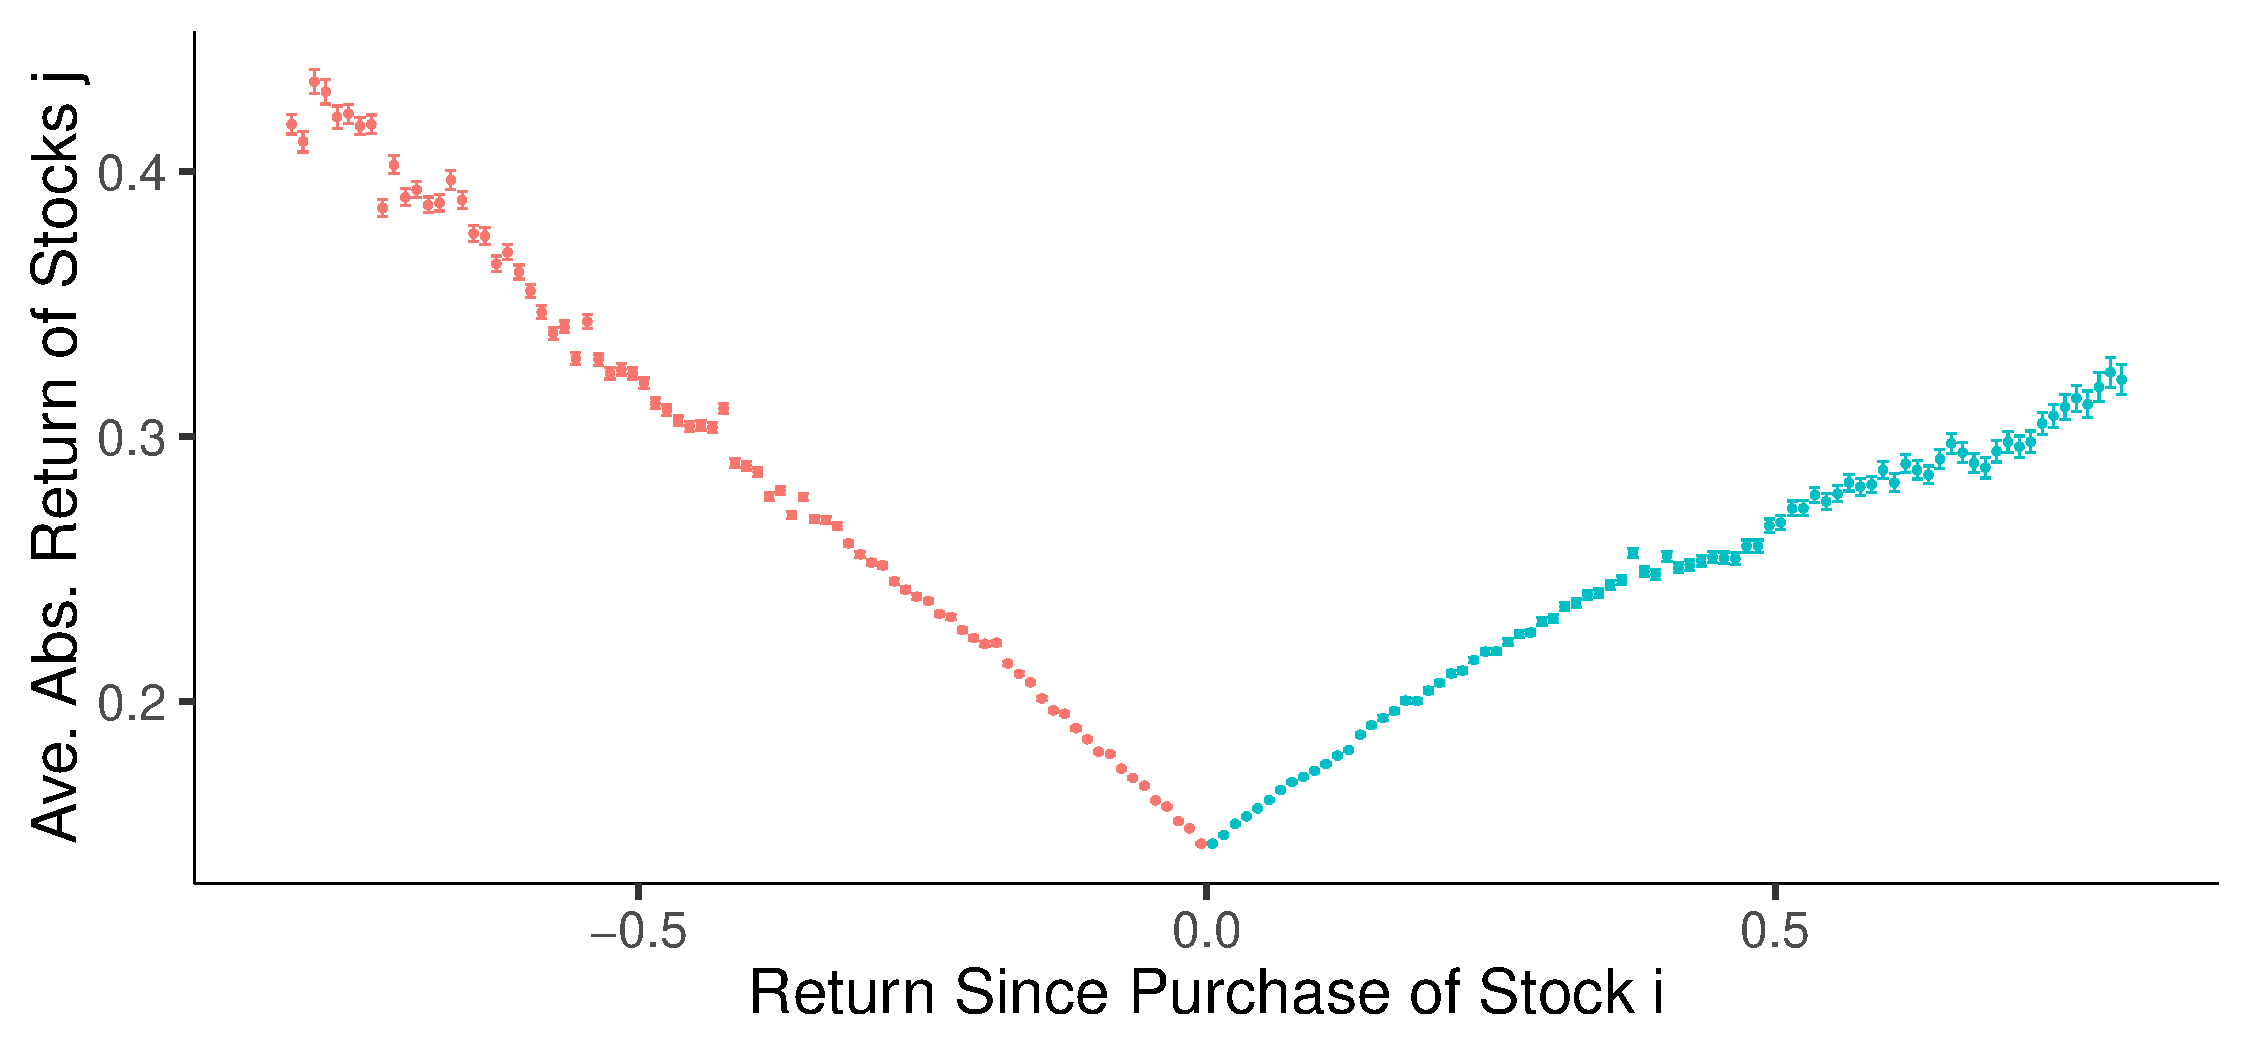
\includegraphics[width=0.8\columnwidth]{barc_R_i_abs_R_j.pdf}
	\caption{Return of stock $i$ and average absolute return of stocks $j$ (Daily portfolio sample given $N\geq2$).}
	\label{figure:ret_i_abs_j}
\end{figure}




\begin{figure}[H]
	\centering
	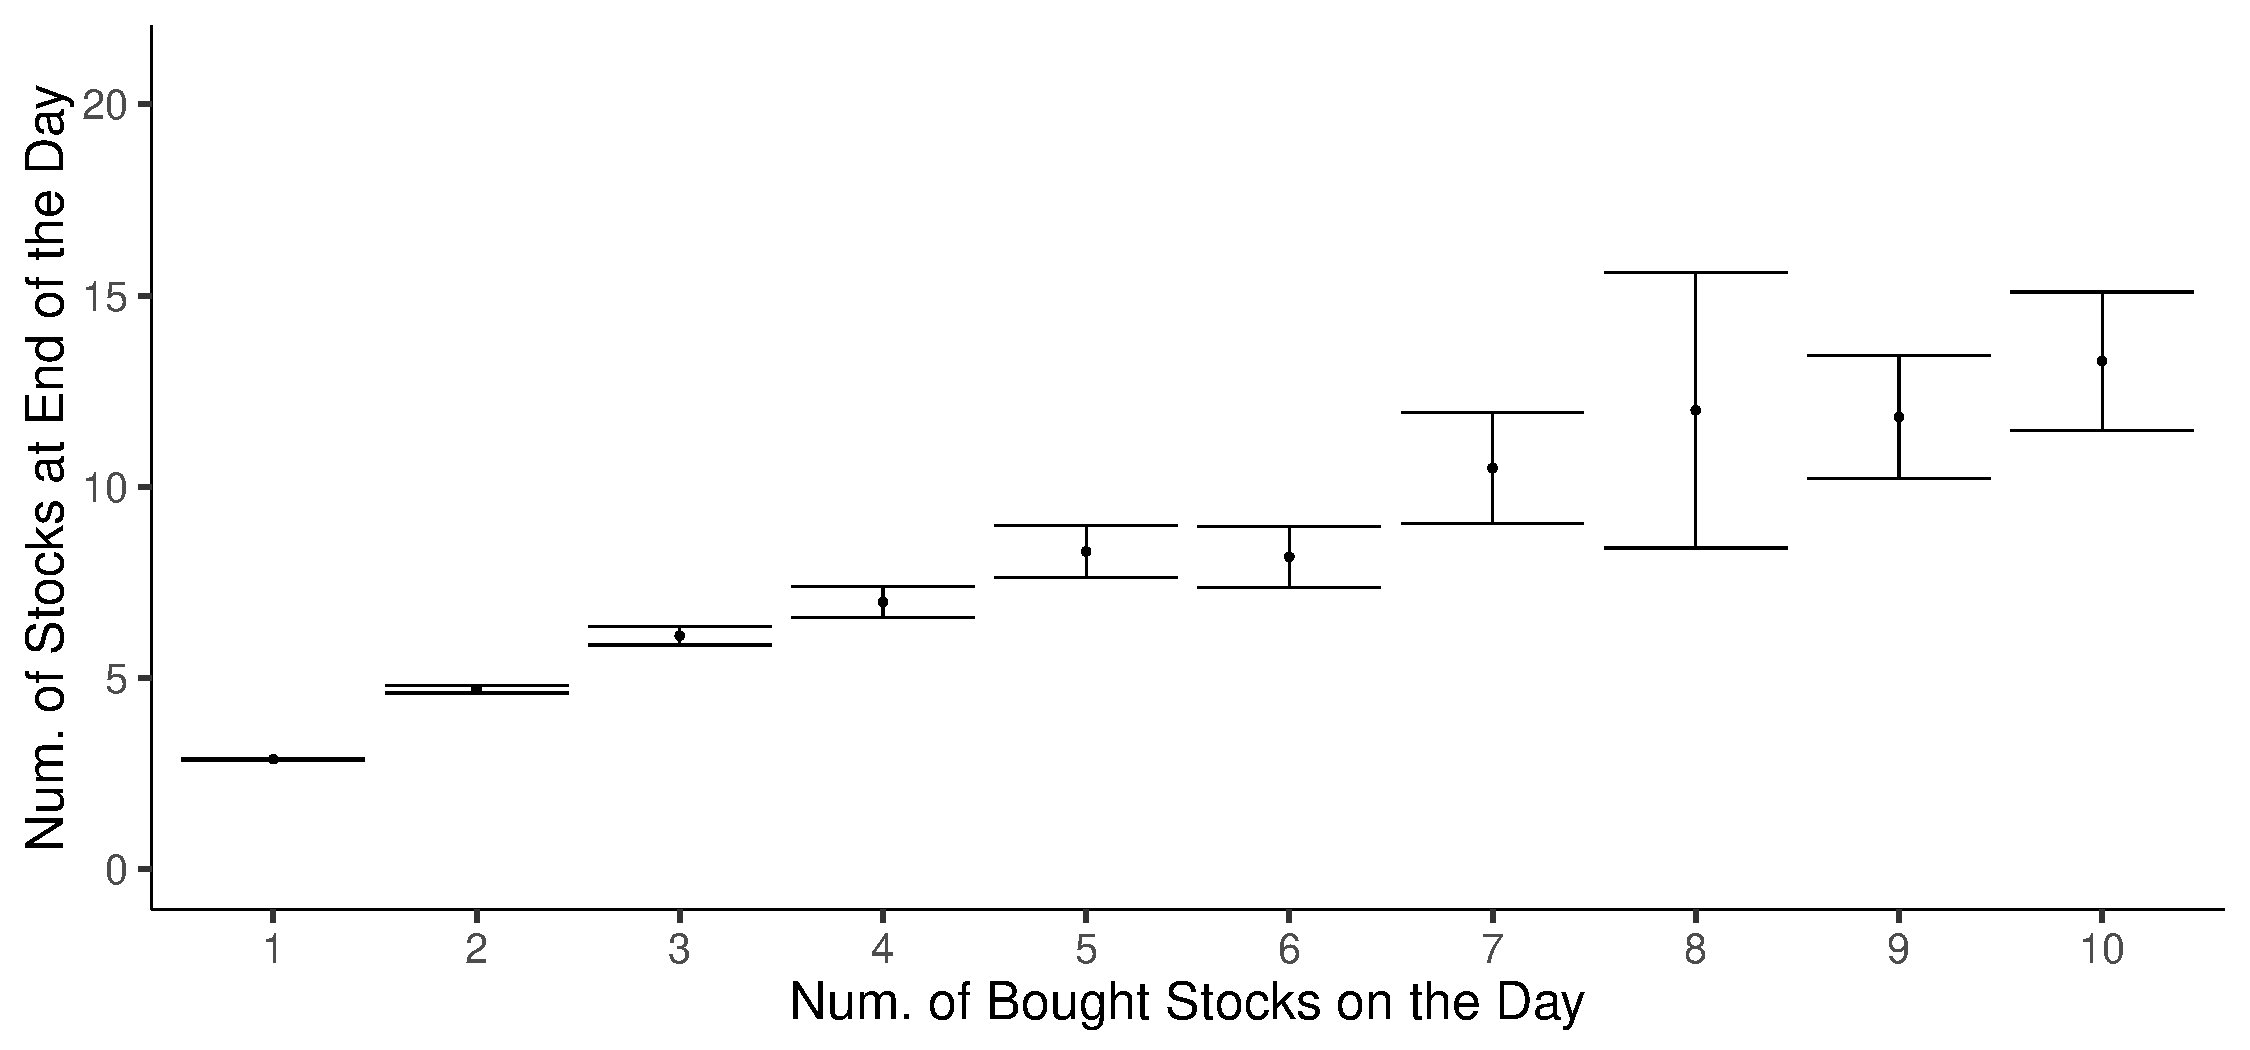
\includegraphics[width=0.8\columnwidth]{barc_buy_days_num_stocks.pdf}
	\caption{Number of Stocks Bought on the Day and Number of End-Day Stocks (Buy-day portfolio sample given $N\leq10$).}
	\label{num_buys_num_stocks}
\end{figure}


\begin{figure}[H]
	\centering
	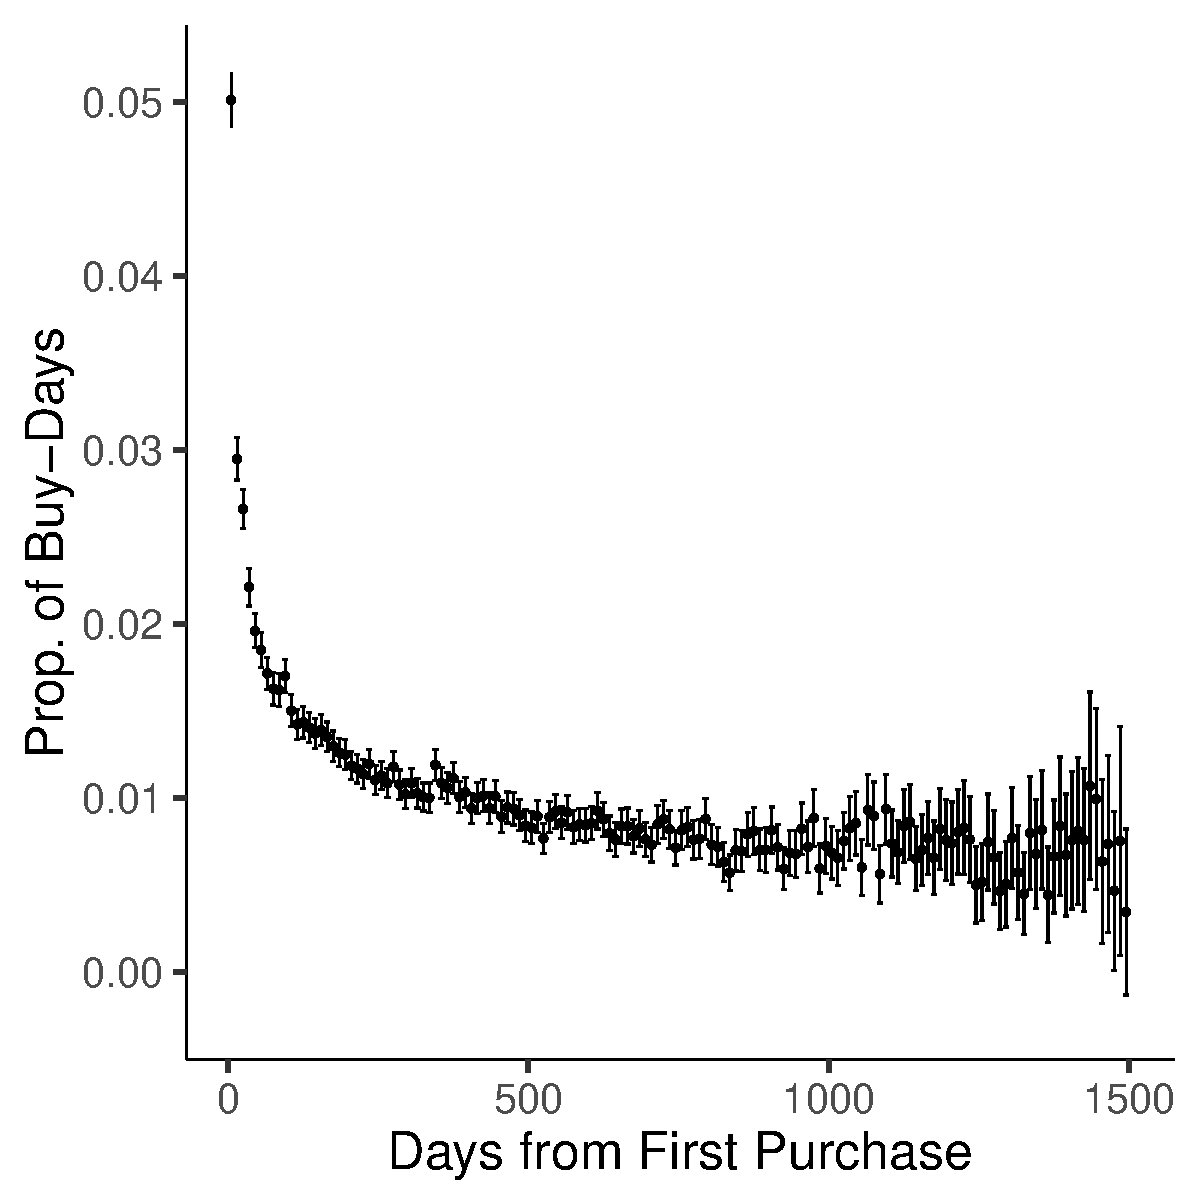
\includegraphics[width=0.6\columnwidth]{barc_prop_buy_fr_first_buy.pdf}
	\caption{Proportion of Buy-Days among All days as a Function of Distance from a First Buy Day (Daily portfolio sample).}
	\label{figure:first_buy}
\end{figure}

\begin{figure}[H]
	\centering
	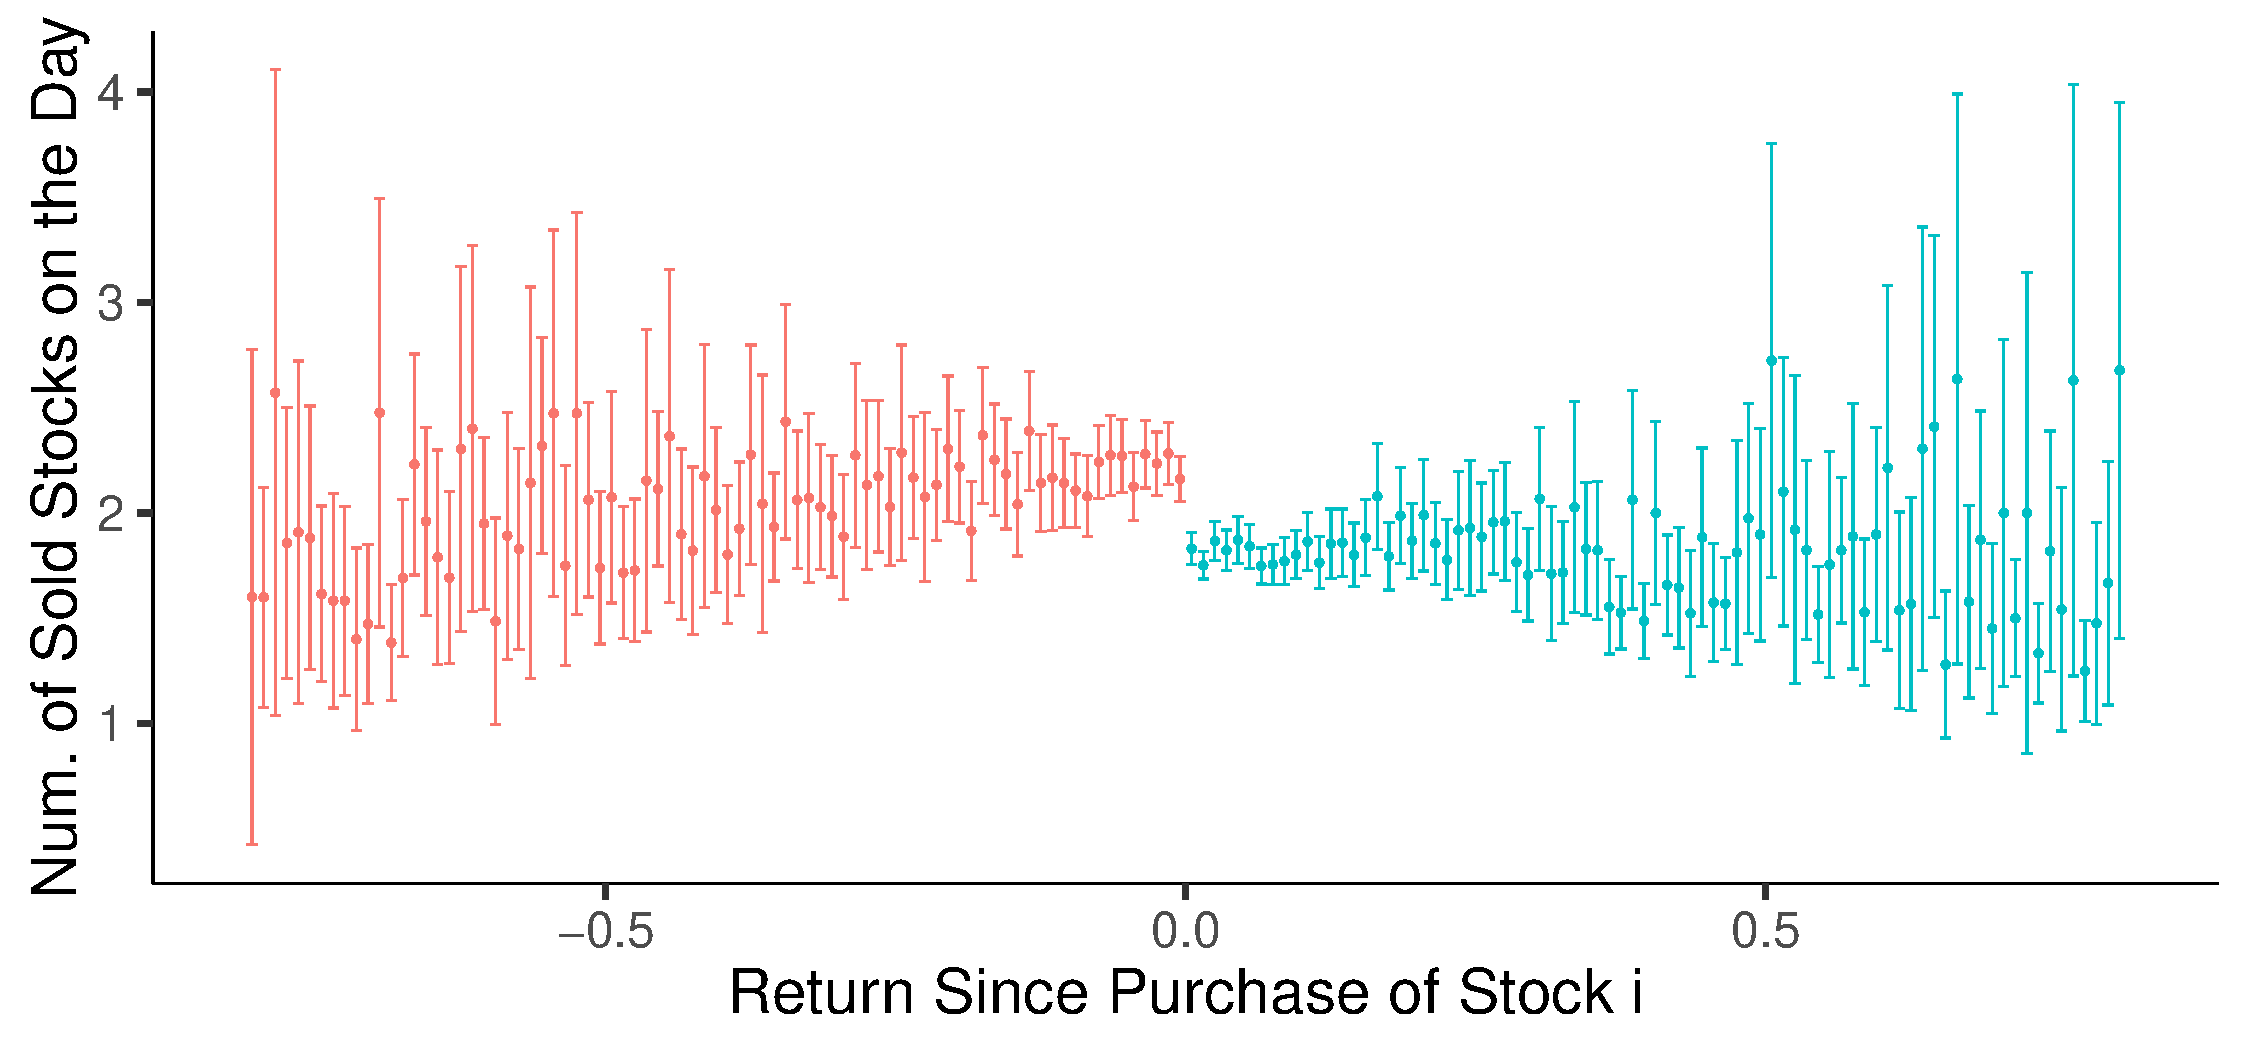
\includegraphics[width=0.8\columnwidth]{barc_num_sold_stocks_given_i_sold_sell_day_NG1_NL1_3.pdf}
	\caption{Number of sold stocks on the day given that stock $i$ is sold.}
	\label{figure:num_sold_given_i_sold}
\end{figure}

